% Date : April 1, 2020
% Author : 
% Subhankar Mishra
% School of Computer Sciences 
% NISER

\documentclass[12pt,a4paper]{report}
\setlength{\oddsidemargin}{0.25in}
\setlength{\evensidemargin}{0.15in}
\setlength{\topmargin}{0.3in}
\setlength{\textwidth}{6.0in}
\setlength{\textheight}{8.5in}
\usepackage{amsmath,amssymb}
\usepackage[printonlyused,withpage]{acronym}
\usepackage{enumitem}
\usepackage{mathptmx}
\usepackage[linguistics]{forest}
\usepackage{mathptmx}
\usepackage{afterpage}

\newcommand\blankpage{%
    \null
    \thispagestyle{empty}%
    \addtocounter{page}{-1}%
    \newpage}

\usepackage[colorlinks]{hyperref}
\usepackage{epigraph}
\usepackage{algpseudocode}
\usepackage{algorithm}
\usepackage{graphicx}
\usepackage{caption}
\usepackage{subcaption}
\usepackage{enumitem}
% \usepackage{subfig}
\usepackage{url}
% \usepackage{feynman}
\usepackage[T1]{fontenc}
\usepackage[utf8]{inputenc}
\usepackage{graphics}
\usepackage{array}
\usepackage{lscape,graphicx}
\usepackage{amsfonts}
\usepackage{longtable}
\usepackage{epsfig}
\usepackage{float}
\usepackage{rotating}
\usepackage{caption}
\usepackage{listings}
\usepackage{mwe} % for blindtext and example-image-a in example
\usepackage{wrapfig}
\usepackage{lipsum}
\usepackage{fancyhdr}
% \usepackage{movie15}
\usepackage{hyperref}
\hypersetup{
    colorlinks = false,
    linkbordercolor = {white},
}
\usepackage{graphicx}
\usepackage{epstopdf}
\epstopdfDeclareGraphicsRule{.gif}{png}{.png}{convert gif:#1 png:\OutputFile}
\AppendGraphicsExtensions{.gif}
\usepackage{lineno}
\usepackage{tikz-qtree}
% \usepackage{biblatex}
\setlength{\headheight}{15pt}
\usepackage[titletoc]{appendix}
% \usepackage[english]{babel}
% \usepackage{biblatex}
% \addbibresource{ref.bib}

% \addto{\captionsenglish}{\renewcommand{\bibname}{References}}

\usepackage{notoccite}   %#To order all the citation on order it is in bibtex


\usepackage{titlesec}
\titlespacing*{\chapter}{0pt}{0pt}{0pt}
\titleformat{\chapter}[display]{\normalfont\huge\bfseries}{\chaptertitlename\ \thechapter}{20pt}{\Huge}

%%%%%%%%%%%%%%%%%%%%%%%%%%%%%%%%%%%%%%%%%%
%%%  macro for margin change
\newenvironment{changemargin}[2]{%
\begin{list}{}{%
%\setlength{\topsep}{0pt}%
\setlength{\leftmargin}{#1}%
\setlength{\rightmargin}{#2}%
%\setlength{\listparindent}{\parindent}%
%\setlength{\itemindent}{\parindent}%
%\setlength{\parsep}{\parskip}%
}%
\item[]}{\end{list}}
%%%%%%%%%%%%%%%%%%%%%%%%%%%%%%%%%%%%%%%%%%

\begin{document}
\begin{changemargin}{0cm}{0cm}
\thispagestyle{empty}
\baselineskip25pt
\begin{center}
{\Large {\bf SEARCH FOR HEAVY RESONANCES USING DEEP NEURAL NETWORK}}\\
\end{center}
\vspace{5mm}
\vfill
\baselineskip15pt
\begin{center}
{\em A thesis Submitted} \\
in Partial Fulfilment of the Requirements \\
for the Degree of \
\vskip .30\baselineskip
{\large{\bf MASTER OF SCIENCE}}
\end{center}
\baselineskip25pt

\vfill
\begin{center} {\bf {\em by}} \\
{\large{\bf Shivam Raj}} \\


{{ \textit{ Under Supervision of:} }}\\
{\large{\bf Dr. Prolay Kr. Mal}}\\
\end{center}

\vfill
\begin{center}
\begin{figure}[h!]
\centering

\includegraphics[scale=0.5]{Figure/NISER.png}
% Reference for the Logo: Student Forms | NISER https://www.niser.ac.in/forms/academic/LaTexTemplate_MScThesis.zip
\end{figure}
 {\bf {\em to the }} \\
{\bf {\large School of Physical Sciences}} \\
{\bf {\large National Institute of Science Education and Research}} \\
{\bf Bhubaneswar} \\
{\bf \today} 
\end{center}
\end{changemargin}



\pagenumbering{roman}
\baselineskip=20pt
\begin{center}
{\bf DECLARATION}
\end{center}

I hereby declare that I am the sole author of this thesis in partial fulfillment of the requirements for a postgraduate degree from National Institute of Science Education and Research (NISER). I authorize NISER to lend this thesis to other institutions or individuals for the purpose of scholarly research.

\vskip1.0in

\hspace*{3.5in} {Signature of the Student} \\
\hspace*{3.5in} {Date:}

\vskip1.0in
\vskip1.0in

The thesis work reported in the thesis entitled .......................................................  was carried out under my supervision, in the school of ............................................... at NISER, Bhubaneswar, India.

\vskip1.0in

\hspace*{3in} {Signature of the thesis supervisor} \\
\hspace*{3in} {School:}\\
\hspace*{3in} {Date:}
% 
\begin{center}
{\large {\bf DEDICATION}} 
\end{center}


\include{stat}
\include{cert1}
\begin{center}
{\bf ACKNOWLEDGEMENTS}
\end{center}
I want to express my deep gratitude to all those people without whom this project would never have been completed. I want to give special appreciation to my supervisor, Dr. Prolay Kr. Mal, to provide me with the opportunity to work in CMS with this exciting work. Also, I want to thank my supervisor for his enthusiasm, support, encouragement, and patience, which help me to complete this project.\\
I would also like to thank the members of my committee: Prof. Sanjay Kr. Swain, Dr. Subhasis Basak, Dr. Yogesh K. Srivastava, and Dr. Amaresh K. Jaiswal for their comments and suggestions.\\
Furthermore, I would like to express special gratitude to Prafulla Saha; without his assistance, this work remains incomplete. I also want to thank Alok Kumar Das, Amit Pal, Chandiprasad Kar, Kuldeep Kumar Pal, Lipsa Rani Panda, Priyanka Mishra, and Tribeni Mishra for their assistance and a healthy discussion over the doubts in the course of this project. Throughout this project, these people help me to clarify the problem and make it simpler for me to understand the reasoning behind the processes. I also want to thank Er. Deepak Kr. Pattanaik for making the humorous, light, and wonderful environment in the lab.\\ 
I would like to thank DAE(India) for providing me with financial support. I also like to express my gratitude to the NISER and SPS, where I learned to develop a research career.\\
I also want to thank my mother, family, and friends for their patience and sacrifices during all this time.


 \begin{flushright}
 Shivam Raj 
 \end{flushright}                   


                                           


\begin{center}
{\large {\bf  ABSTRACT }}

\end{center}  


 
%  Extracting signals which is in a small cross-section compared to the large cross-section of the background processes has been helped by introducing machine learning (ML) techniques for classification purposes. Classification algorithms in machine learning is a type of supervised learning where the outputs are constrained only to a limited set of values or classes such as signals or backgrounds. In this thesis, the classification of the produced heavy resonances from  collision at the Large Hadron Collider(LHC) is presented. The machine learning technique, deep neural network(DNN), is used to classify the resonances from the background processes. Heavy resonances such as Vector-like quark(VLQ), Tprime () at different mass points [600, 1200] GeV are used as the signal while Standard model Higgs(SMH) and Non-Resonant background(NRB) as the backgrounds for the training and testing of the DNN model. On the DNN output variable, the expected limit has been calculated using Higgs Combined Tools under the  environment. Preliminary studies shows DNN can have a better/comparable results to other machine learning techniques used for the high energy physics analysis. 
%  DNN seems to sensitivity in signal-background separations and the expected limit than the other machine learning techniques Boosted Decision Trees(BDT). The DNN and BDT performance have been used to search H $\longrightarrow$ $\gamma\gamma$ in the leptonic channel.

Extracting signals in a small cross-section compared to the large cross-section of the background processes has been helped by introducing machine learning (ML) techniques for classification purposes. Classification algorithms in machine learning is a type of supervised learning where the outputs are constrained only to a limited set of values or classes such as signals or backgrounds. This thesis presents the classification of the produced heavy resonances from $pp$ collision at the Large Hadron Collider(LHC). The machine learning technique, deep neural network(DNN), is used to classify the resonances from the background processes. Heavy resonances such as Vector-like quark(VLQ), Tprime ($T'$) at different mass points [600, 1200] GeV are used as the signal while Standard model Higgs(SMH) and Non-Resonant background(NRB) as the backgrounds for the training and testing of the DNN model. On the DNN output variable, the expected limit has been calculated using Higgs Combined Tools under the \texttt{CMSSW} environment. Preliminary studies show DNN can have a better/comparable results to other machine learning techniques used for the high-energy physics analysis.
\clearpage
\fancyfoot{}      % Delete current footer settings

\pagestyle{fancyplain}
 \renewcommand{\chaptermark}[1]{\markboth{\thechapter\ #1}{\thechapter\ #1}} % remember chapter title
 \lhead[\fancyplain{}{}]{\fancyplain{}{}}
 \rhead[\fancyplain{}{}]{\fancyplain{}{\em\leftmark }}
 \renewcommand{\headrulewidth}{0.3pt}
 \cfoot{\rm\thepage} % page number

\baselineskip=12pt
\tableofcontents
\clearpage
\listoffigures
\clearpage
\listoftables 
\clearpage
\pagenumbering{arabic}
\baselineskip=24pt

\chapter{\label{intro}Introduction}

High energy physics is about understanding elementary particles that are fundamental constituents of matter.  Experimental high-energy physics (HEP) focuses on two primary interconnected goals, which seek novel particles associated with physics beyond the Standard Model(BSM) and Standard Model(SM) particles with high precision\cite{Salam:1964ry}\cite{GLASHOW1961579}. The standard model had correctly predicted the existence of $W^\pm$ and Z bosons along with the top quark\cite{PhysRevLett.19.1264}\cite{10.1143/PTP.49.634}. The Higgs boson discovery in 2012 at the LHC(CERN) further upholds the model\cite{Aad_2015}\cite{Aad_2014}.

\autoref{fig:my_figure_1} lists standard model particles with the known three generations of leptons and quarks, the gauge bosons, and Higgs boson. The leptons and quarks make up matter, whereas the gauge bosons mediate the interactions among them\cite{PhysRevLett.13.321}. All massive fundamental particles in the Standard Model get their masses through the Brout-Englert-Higgs (BEH) mechanism\cite{Higgs:1964pj}.

For SM and BSM, rare signals need to be identified from vast backgrounds. This becomes an important issue as the number of pile-up collisions with additional protons in the bundle at  HL-LHC increases significantly\cite{https://doi.org/10.48550/arxiv.1807.02876}. This have been helped by the introduction of machine learning techniques. Machine learning algorithms are state-of-the-art in event and particle identification, energy estimation, and pile-up suppression applications in HEP. By using machine learning techniques to study the laws governing the structure of matter and  its interactions\cite{Baldi2014}.

Observing and studying these particles can reveal crucial information on the nature of matter\cite{Higgs_snowmass}. Such discoveries necessitate the use of sophisticated statistical approaches, and the use of machine learning tools. Improvements in analytical techniques immediately raise particle discovery potential, given the limited quantity and high cost of data.



% Chapter 1: Introduction
%     \begin{itemize}
%         \item SM
%         \item BSM
%         \item VLQ
%         \item Signal and Background Topology 
%         \item CMS
%         \item Objective of your experiment
%             \end{itemize}
    
% chapter 2: Machine Learning
% Chapter 3:  Simulated Samples
% \begin{itemize}
%     \item About CMS
%     \item about how can it be helpful for your work
%     \item how data are simualtad 
%     \item how you obtained the data
%     \item as written in the last report

% \end{itemize}

% Chapter 4:Analysis Strategies\\

% chapter 5:- Results and Discussion\\
% ch-6: summary and Conclusion



\section{Standard Model and shortcomings}

The Standard Model of particle physics(\autoref{fig:my_figure_1})is a model attempt to explain events and phenomena in the universe. The Standard Model(SM) of fundamental interaction, which has been successfully tested for the past 30 years, confirms its dynamics in the gauge sector and flavour structure, including a compelling confirmation of the reason of observable parity violations(P) and coupled charge and parity symmetry(CP). However, this is an incomplete theory and does not explain many  observed or unobserved events, such as:
\begin{figure}[H]
    \centering
    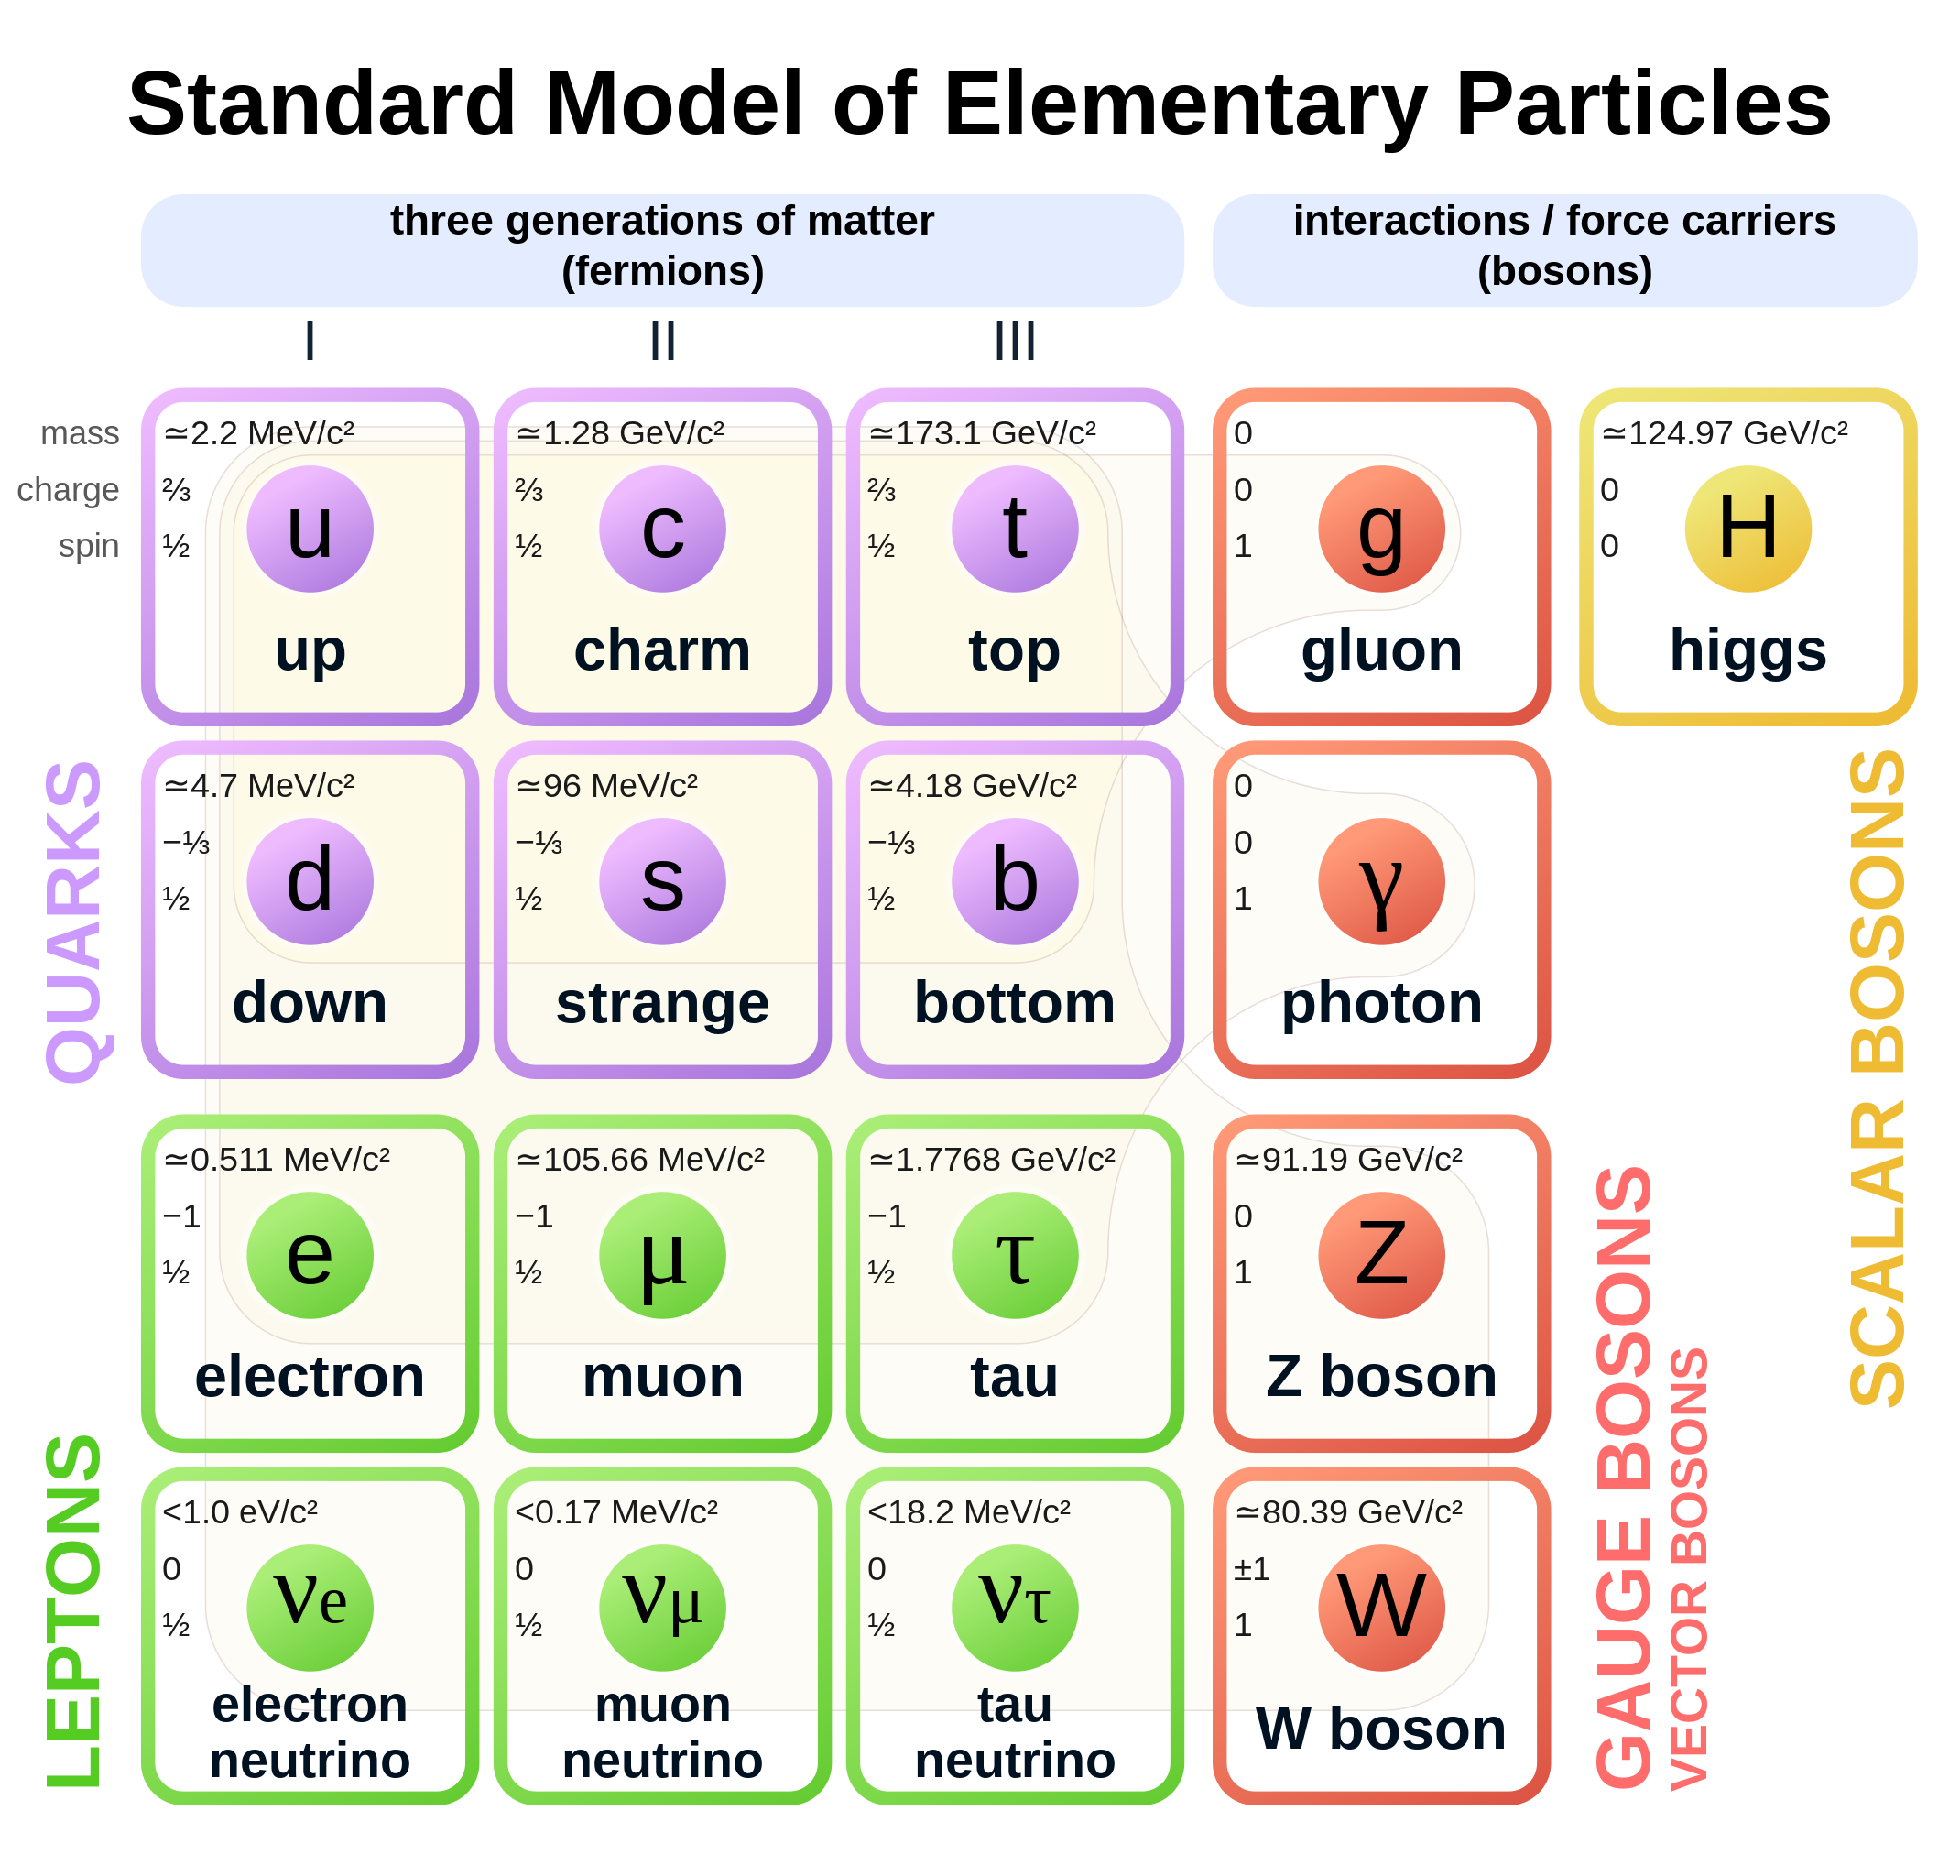
\includegraphics[scale =0.1]{figure_1/Standard_Model_of_Elementary_Particles.svg.png}
    \caption{Figure represent Standard model of particle physics. This includes three generation of quarks and leptons, along with force mediator gauge Boson, photon, and gluon. It also include the scalar Higgs bosons.}
    \label{fig:my_figure_1}
\end{figure}
\begin{itemize}
    \item \textbf{Gravity:-} The Standard Model does not consistently explain the canonical theory of gravity and the general theory of relativity from the perspective of quantum field theory, despite the fact that it corresponds to strong interaction and electroweak interaction \cite{Bilson_Thompson_2007}. The fact that quantum field theory in the field of gravity frequently collapses before reaching the Planck scale is one reason for this. As a result, we don't have a solid theory for the origins of the universe.
    
    \item \textbf{Hierarchy problem:-} The Higgs field causes spontaneous symmetry violation in the Standard Model, which introduces particle mass\cite{Higgs:1964pj}. Due to the presence of virtual particles in the Standard Model, the Higgs mass experiences substantial quantum corrections (top quarks). These adjustments are substantially larger than the Higgs real mass.\cite{Aad_2015}. 

\item \textbf{Neutrino Oscillation:-} According to the standard model, neutrinos have zero mass. But, from experiments and studies conducted in past decades have evidenced to have neutrino mass. Manually adding the neutrino mass term to the Standard Model creates a new theoretical problem\cite{neutino_1}. For example, the mass term must be very small, and it is unclear if the mass of neutrinos is generated in the Standard Model in the same way as the mass of other constituent particles\cite{Ellis_2020}.
    
    
 \item \textbf{Matter anti-Matter asymmetry:-} The universe is mainly composed of matter. However, the Standard Model predicts that if the initial conditions of the universe do not contain an imbalanced amount of matter compared to antimatter, matter and antimatter should be formed in (almost) equal amounts\cite{Dasgupta_2020}. However, the Standard Model does not have a mechanism to properly explain this asymmetry.

There are many other observed phenomena without evident explanation by the standard model, such as strong CP problem\cite{doi:10.1126/science.abk1781}, presence of Dark matter and Dark energy, and the most recent anomalous mass of the W boson-results from the CDF Collaboration\cite{CMS:2008xjf}.
\end{itemize}   



The Beyond Standard Model (BSM) needs to address phenomena that cannot be explained by the Standard Model, such as  strong CP problems, neutrino oscillations, matter-antimatter asymmetry, and the inability to explain the properties of dark matter and dark energy. \cite{https://doi.org/10.48550/arxiv.1202.1391}. Many theories have been developed to extend  SM to address some of the above issues. Some of these models are supersymmetry (SUSY)\cite{MARTIN_1998}, right-handed neutrino seesaw models \cite{neutrino_mass_model}, vector-like quarks, and extra-dimensional prediction models. Vector like Quark (VLQ) model predicts the presence of giant particles, Non-chiral quark. Proton-proton(pp) collisions can form these quarks at 13 TeV at the LHC. VLQ is the primary focus of this analysis and will be discussed in detail in the following sections.



%  Surprisingly, all these extensions of  SM predict new particles. The SUSY model predicts the presence of  supersymmetric partners for all SM particles with different spin  units. This means that all fermions have supersymmetric boson partners and vice versa. 
%  The seesaw model introduces a sterile heavy right-handed neutrino to explain this much. 
%  A small left-handed neutrino mass that appears in  SM. The additional dimensions predict the existence of some new dimensions in addition to the usual four space-time dimensions. These may explain why gravity is so much weaker than  other fundamental forces of nature. According to these theories, gravitons (carriers of gravitational force) can penetrate these additional dimensions, but other SM particles cannot. Vectorlike Quark (VLQ) model predicts the presence of giant particles  Non-chiral quark. These quarks can be formed by proton-proton (pp) collisions at 13 TeV at the LHC. VLQ is the subject of this research and will be discussed in detail in the next section.

\section{Vector-like Quarks(VLQ)}

Standard model(SM) is consists of only chiral fermions, where the left-handed and right-handed fermionic fields are conserved, which transform differently under the SU(2) gauge transformations. As a result, the Dirac mass term m becomes $\psi\Bar{\psi}$\cite{Aguilar_Arevalo_2018}. SM with charged fermions gain mass via the (BroutEnglertHiggs) BEH mechanism\cite{PhysRevLett.13.321}\cite{Higgs:1964pj}. In particular,  W bosons only interact with SM left-handed fermions. 

However, some theoretical models predict the existence of new heavy quarks that are not Chiral
in nature. Such models include compound Higgs\cite{10.3389/fphy.2019.00022}, Randall Sundrum
models\cite{Randall_1999}, and Grand Unified Theory (GUT)\cite{Kang_2008} and Little Higgs
model\cite{Arkani_Hamed_2002}. Unlike SM quarks, these quarks are Vector coupled to the charged current. These quarks are heavier partners for top and bottom quarks\cite{Angelescu_2016}. That is, a $T'$ quark with a charge of $ \frac{2}{3} $ e and a $B'$ quark with a charge of $ -\frac{1}{3} $ e. These predicted models help to cancel the divergent quantum loop correction introduced by the top quark into the Higgs mass. These new quarks can interact with SM particles and  decay to one-third generation quarks and  heavy bosons. For such non-chiral fermions, the Dirac mass term m $ \psi\Bar{\psi} $ is not prohibited. The only way to determine the mass of these particles is to find them experimentally.  Previous searches for these VLQs were performed by both ATLAS and CMS at the center of mass energy ($ \sqrt{s}$) = 7, 8, and 13TeV \cite{Aad_2014}. It is a colored spin 1/2 fermion \cite{VLQ_1}. 
% The left-handed and right-handed components are transformed in the standard model gauge group as well. Therefore different SM chiral quarks, their masses are not produced by the Yukawa interaction with the Higgs. 
%  It is a  boson and has little effect on the cross-section of the Higgs boson. Various modifications 
%  The new physics els introduces vector-like quarks. 
%  Such models include composite Higgs models \cite{neutrino_mass_model}, Little-Higgs model \cite{Perelstein_2004} \cite{Matsedonskyi_2013},  Extradimension model [\cite{Randall_1999}, etc. 
%  This paper investigates the specific separation of the Tprime ($T`$) quark decay topology  described in the next section.
 
 
 







The vector-like top quark partner $T'$ has two generation modes, as shown in \autoref{fig:threeVLQgraphs}\cite{Belyaev_2021}. One is due to
pair production where  there is a strong interaction(\autoref{fig:threesinx}) and the other is a single production mode
with electroweak interactions(\autoref{fig:yequalsx}). The VLQ pairs to SM quarks q and weak bosons V$\in$ \{W, Z, H \},
via QqV vertices, as shown in \autoref{fig:threeVLQgraphs} and in \autoref{eq:label_1222}

\begin{equation*}\label{eq:label_1222}
\begin{split}
 T' \longrightarrow tW, T' \longrightarrow tZ, T' \longrightarrow tH  \\
   B' \longrightarrow bW, B' \longrightarrow bZ, B' \longrightarrow bH
\end{split}
\end{equation*}


\begin{figure}[H]
     \centering
     \begin{subfigure}[b]{0.47\textwidth}
         \centering
         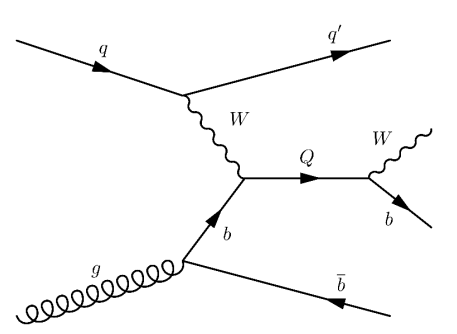
\includegraphics[width=\textwidth]{figure_1/1.png}
         \caption{Single production of VLQ, $T'$.}
         \label{fig:yequalsx}
     \end{subfigure}
     \hfill
     \begin{subfigure}[b]{0.47\textwidth}
         \centering
         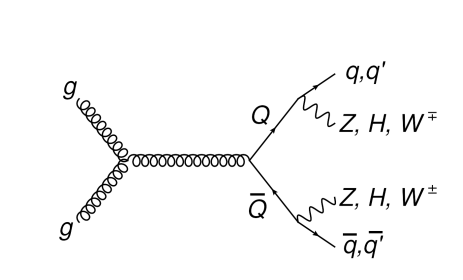
\includegraphics[width=\textwidth]{figure_1/2.png}
         \caption{Pair production of VLQ, $T'$.}
         \label{fig:threesinx}
     \end{subfigure}
     \hfill
    %  \begin{subfigure}[b]{0.3\textwidth}
    %      \centering
    %      \includegraphics[width=\textwidth]{graph3}
    %      \caption{$y=5/x$}
    %      \label{fig:five over x}
    %  \end{subfigure}
        \caption{The different mode of generation modes of the vector-like quark, $T'$.}
        \label{fig:threeVLQgraphs}
\end{figure}





The $T'$ quark combined with tW, tZ, or tH into the corresponding $T'$ quark. 
 In this thesis, the study  has been considered with a single VLQ, top quark partner $T'$  generated in a proton-proton (pp) collision at the center of mass energy ($\sqrt{s}$) = 13TeV, with processes pp $\longrightarrow$ $T'$ at LHC(discussed in \autoref{CMS}). The focus is on electroweak generation, $T'$ qH channel from the Higgs boson to two photons (H $\longrightarrow\gamma\gamma$) and is generated by the Higgs boson decay $T'$ $\longrightarrow$ tH. The leading order (LO) Feynman diagram for the $T'$ is shown in \autoref{fig:my_label_Feynman}. This analysis is designed to be sensitive to  top quark lepton decay and Higgs boson decaying into two photons. The experimental features are the resonance peak of the invariant mass spectrum of the two photons and another resonance peak of the invariant tH  mass spectrum. A detailed description of $T'$ and the corresponding backgrounds can be seen in \autoref{signal_background}. 
The separation of signal, for the $T'$ quark from the large backgrounds processes have been helped with the use Deep neural network(DNN) which have been discussed briefly in next section.


   




\begin{figure}[H]
    \centering
    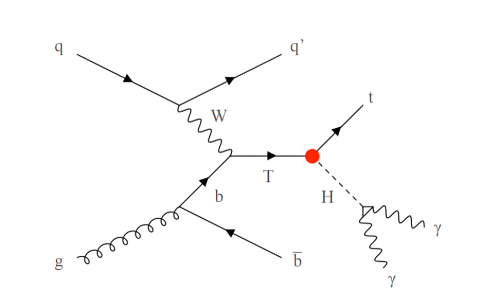
\includegraphics{figure_4/3.png}
    \caption{Feynman diagram for single vector-like quark(VLQ), ${T'}$ production. $T'$ is produced with the electroweak interaction of W boson and b quark. As being a resonance particle, $T'$ decay in moment into Higgs boson(H) and standard model top quark(t). Higgs(H) further goes on giving diphoton($\gamma\gamma$, while top quark decays to b quark and W boson. W boson decays leptonically to electron(e) and electron neutrino($\nu_e$).}
    \label{fig:my_label_Feynman}
\end{figure}

\section{Deep Neural Network(DNN)}
Neural networks, also known as artificial neural networks(ANN), are structures inspired by the human brain and also mimic the connectivity of biological signals to one another, as in \autoref{fig:my_label_NN_ANNN}.
In the neural network, node takes the input as a real number (the weighted sum of the connected outputs from the previous layer) and performs a non-linear transformation to form that output\cite{Bourilkov_2019}.
These non-linear transformation functions are known as the activation function. A typical activation function is: Sigmoid (logistics) and Tanh (output is limited to the following for all input values), and the normalized linear unit ReLU(max(0, x)) or the positive part of the argument. Each neural network consists of at least an input, an output, and one or more hidden layers\cite{Sarker2021}. This is part of Deep learning. We represent deep NN as DNN. The learning can be supervised depending on pairs of inputs with known outputs for training, or unsupervised, or semi-supervised. A cost or loss function measures the “distance” between the current and the desired outcomes, where our main goal is to make a model loss as little as possible to train the model. Traditional optimization aims to minimize the cost function of available (training) data. The main goal of ML is to generalize or minimize the cost of hidden or test data. At each step,  backpropagation based on the differential chain rule can adjust the weights of all edges to reduce the cost function slightly. This is Stochastic Gradient Descent (SGD), which further in detailed discussed in \autoref{ML}. 
Aside from being universal approximators (i.e., they estimate probability densities or posterior probabilities to arbitrary precision), neural networks are an extremely useful tool due to the short computational time required in their training ( in a majority of applications in HEP)\cite{https://doi.org/10.48550/arxiv.2003.05199}. The DNN has been used for the signal and background separation, which have discussed briefly in next section and in detailed \autoref{signal_background}.
\begin{figure}[h]
    \centering
    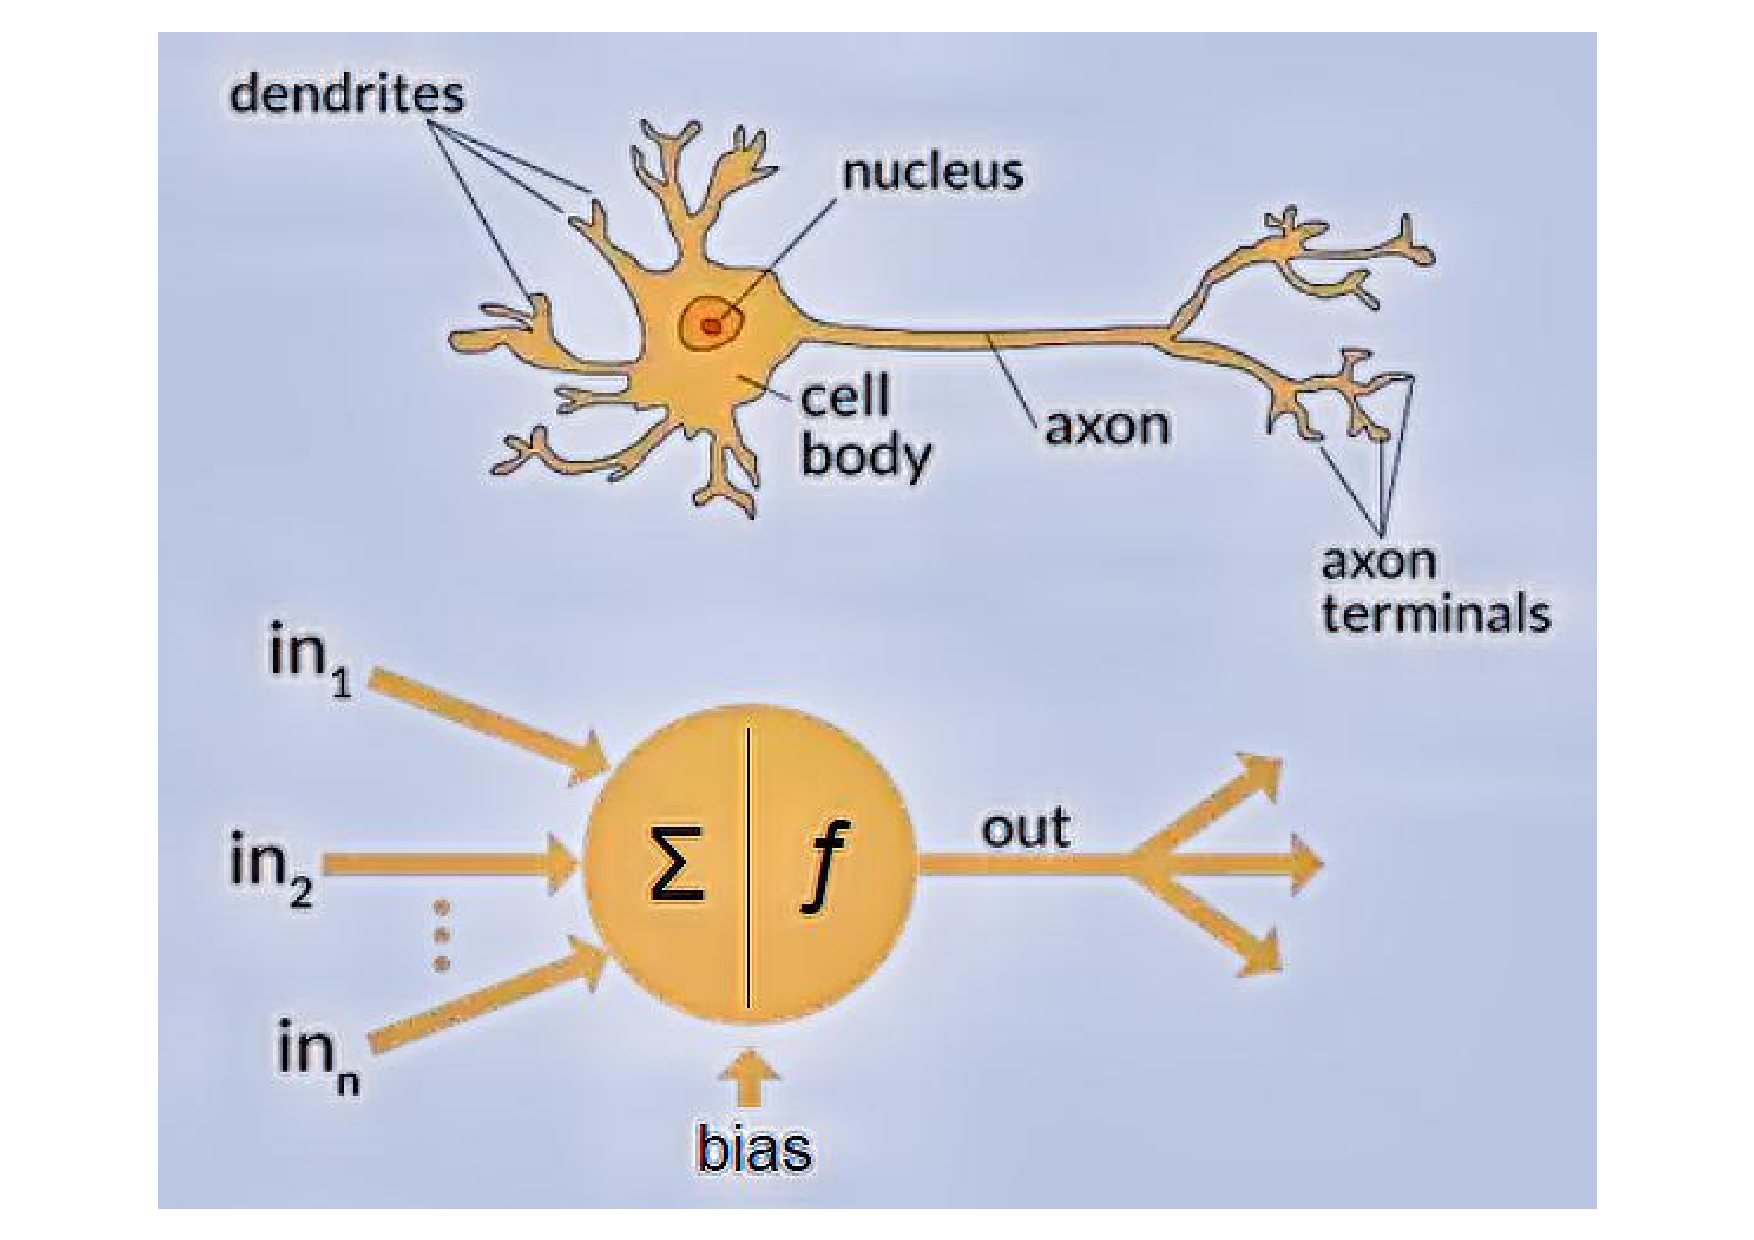
\includegraphics[scale=0.4]{Figure/img_neuron.pdf}
    \caption{A biological and an artificial neuron}
    \label{fig:my_label_NN_ANNN}
\end{figure}

\section{Signal and Background}

The Deep Neural network(DNN) has been trained with the Tprime($T'$) at different mass point from [600,1200]GeV as signal and standard
model higgs(SMH) as the backgrounds which also decays to the leptons. The different SMH backgrounds used in training are
ttH($\longrightarrow$ $\gamma \gamma$), tH($\longrightarrow$ $\gamma \gamma$)q, VBFH($\longrightarrow$ $\gamma \gamma$),
VH($\longrightarrow$ $\gamma \gamma$), and ggH(H($\longrightarrow$ $\gamma \gamma$). All of samples(signal and background) have the
similar final state topology with H $\longrightarrow$ $\gamma \gamma$.

The DNN training model output tested over the Non-Resonant background(tt$\gamma \gamma$, ttJets, tgJets, gJets, and DiphotonJets), which plotted as ratio plot after normalizing with the data and the monte carlo, which have been further discussed in details in \autoref{signal_background}. 


%%%Objective of the experiment%%%% 
The analysis strategy adopted in this thesis with the discussion of the combined tools used for the statistical limit calculation on each mass points of the $T'$ from [600, 1200] GeV are discussed in \autoref{AN}. The DNN model have been compared with the existing analysis using another multivariate techniques, Boosted Decision Tree(BDT) and the output results can be seen in the \autoref{R_D}. The expected limit at 95\% confidence intervals(CLs) on $T'$ production processes have been extracted at each $T'$ mass in the range [600,1200] using the DNN based selection criteria, as well as for the present CMS analysis(BDT).
















    







% \url{https://lhc-machine-outreach.web.cern.ch/lhc_in_pictures.htm}
% \url{https://lhc-closer.es/taking_a_closer_look_at_lhc/1.standard_model}


% \noindent\fbox{%
%     \parbox{\textwidth}{%
% 1.   Dawson, S. et al. Higgs Working Group Report of the
% Snowmass 2013 Community Planning Study, Preprint at
% http://arxiv.org/abs/1310.8361 (2013).
% https://home.cern/science/physics/matter-antimatter-asymmetry-problem
% 2. Neyman, J. & Pearson, E. Philosophical Transactions of
% the Royal Society 231, 694–706 (1933).
% 3.  Womersley, J. (February 2005). "Beyond the Standard Model" (PDF). Symmetry Magazine. Archived from the original (PDF) on 2007-10-17. Retrieved 2010-11-23.
% 4. S. P. Martin, Adv. Ser. Direct. High Energy Phys.21 (2010), 1-153, arXiv:hep-ph/9709356.
% 5 S.F. King, Rept.Prog.Phys. 67 (2004) 107-158, arXiv:hep-ph/0310204
% 6 M. Shifman, Int.J.Mod.Phys.A25:199-225, 2010, arXiv:0907.3074.
% R. Contino, L. Da Rold, and A. Pomarol, “Light custodians in natural composite Higgs
% models”, Physical Review D 75 (March, 2007) 055014,
% doi:10.1103/PhysRevD.75.055014. arXiv: hep-ph/0612048.
% [6] R. Contino, T. Kramer, M. Son, and R. Sundrum, “Warped/Composite Phenomenology
% Simplified”, Journal of High Energy Physics 2007 (May, 2007) 074–074,
% doi:10.1088/1126-6708/2007/05/074. arXiv: hep-ph/0612180.
% [7] D. B. Kaplan, “Flavor at ssc energies: A new mechanism for dynamically generated
% fermion masses”, Nuclear Physics B 365 (November, 1991) 259–278,
% doi:10.1016/S0550-3213(05)80021-5.
% [8] M. J. Dugan, H. Georgi, and D. B. Kaplan, “Anatomy of a composite Higgs model”,
% Nuclear Physics B 254 (January, 1985) 299–326,
% doi:10.1016/0550-3213(85)90221-4.
% [9] S. Blasi and F. Goertz, “Softened Goldstone-Symmetry Breaking”, Physical Review Letters
% 123 (November, 2019) 221801, doi:10.1103/PhysRevLett.123.221801. arXiv:
% 1903.06146.
% [10] M. Perelstein, M. E. Peskin, and A. Pierce, “Top Quarks and Electroweak Symmetry
% Breaking in Little Higgs Models”, Physical Review D 69 (April, 2004) 075002,
% doi:10.1103/PhysRevD.69.075002. arXiv: hep-ph/0310039.
% [11] O. Matsedonskyi, G. Panico, and A. Wulzer, “Light Top Partners for a Light Composite
% Higgs”, Journal of High Energy Physics 2013 (January, 2013) 164,
% doi:10.1007/JHEP01(2013)164. arXiv: 1204.6333.
% [12] M. Schmaltz and D. Tucker-Smith, “Little Higgs Review”, Annual Review of Nuclear and
% Particle Science 55 (December, 2005) 229–270,
% doi:10.1146/annurev.nucl.55.090704.151502. arXiv: hep-ph/0502182.
% [13] L. Randall and R. Sundrum, “A Large Mass Hierarchy from a Small Extra Dimension”,
% Physical Review Letters 83 (October, 1999) 3370–3373,
% doi:10.1103/PhysRevLett.83.3370. arXiv: hep-ph/9905221.
%     }%
% }
\clearpage
\chapter{\label{CMS}The CMS Detector}
The  Large Hadron Collider (LHC), 27 km long, is the largest and most powerful particle accelerator ever manufactured. Accelerate the protons  clockwise and counterclockwise to near the speed of light, causing them to collide at four different positions around the ring, as shown in \autoref{fig:my_label_LHC}. At these points, the energy of the collision of the particles is converted to mass and the particles are sprayed in all directions \cite{CMS_1}. The Compact Muon Solenoid (or CMS) detector is located at one of these four collision points. It was designed to observe  new physical phenomena that the LHC may reveal. The CMS acts as a giant high-speed camera, taking 3D "photographs" of particle collisions from all directions up to 40 million times per second. Most of the particles produced by the collision are "unstable" and short-lived, but quickly turn into stable particles that can be detected by the CMS.\cite{CMS_1}-\cite{CMS:2008xjf}.\\
 CMS is 15 meters in diameter. CMS magnets are the central device on which experiments are built, with a magnetic field of 4 Tesla about $10^6$ times stronger than Earth.\cite{CMS:2008xjf}\cite{CMS_2}.
 \begin{figure}[H]
     \centering
     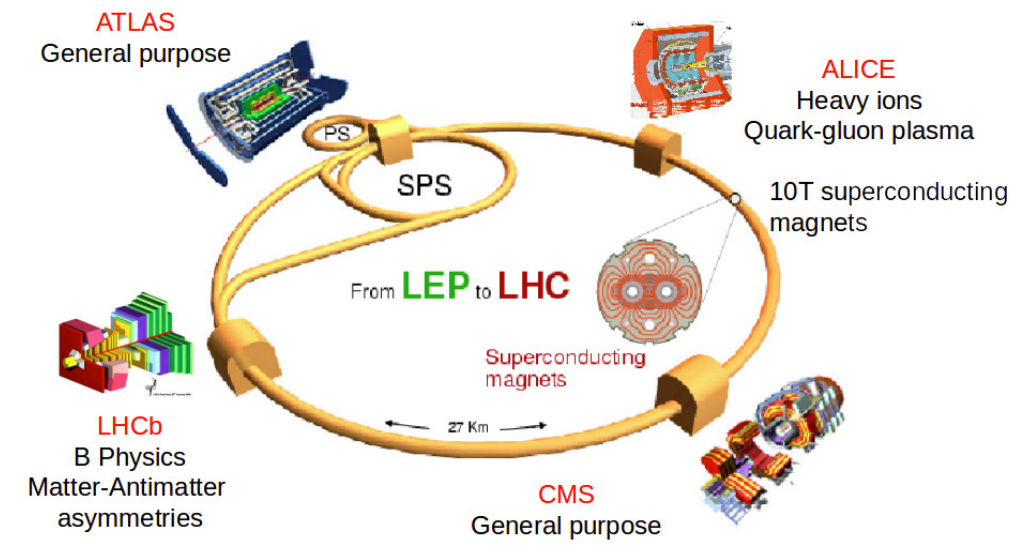
\includegraphics[scale=0.3]{Detector/14__ml.png}
     \caption{LHC}
     \label{fig:my_label_LHC}
 \end{figure}
A magnetic field is used to track the path of a particle to measure its momentum. The greater the amount of exercise, the less bending \cite{CMS_1}. The greater the momentum of a particle, the less likely it is that the  path will be curved by a magnetic field. Therefore, following that path gives a measurement of particle momentum. The tracker and calorimeter detectors (ECAL and HCAL) fit snugly inside the magnetic coil, and the muon detector surrounds the magnetic coil and is inserted into a 12-sided iron structure that  contains and guides the magnetic field(as can be seen from the \autoref{fig:my_label_detect})\cite{CMS_2} and in \autoref{fig:my_label_CMS}.
\begin{figure}[h]
    \centering
    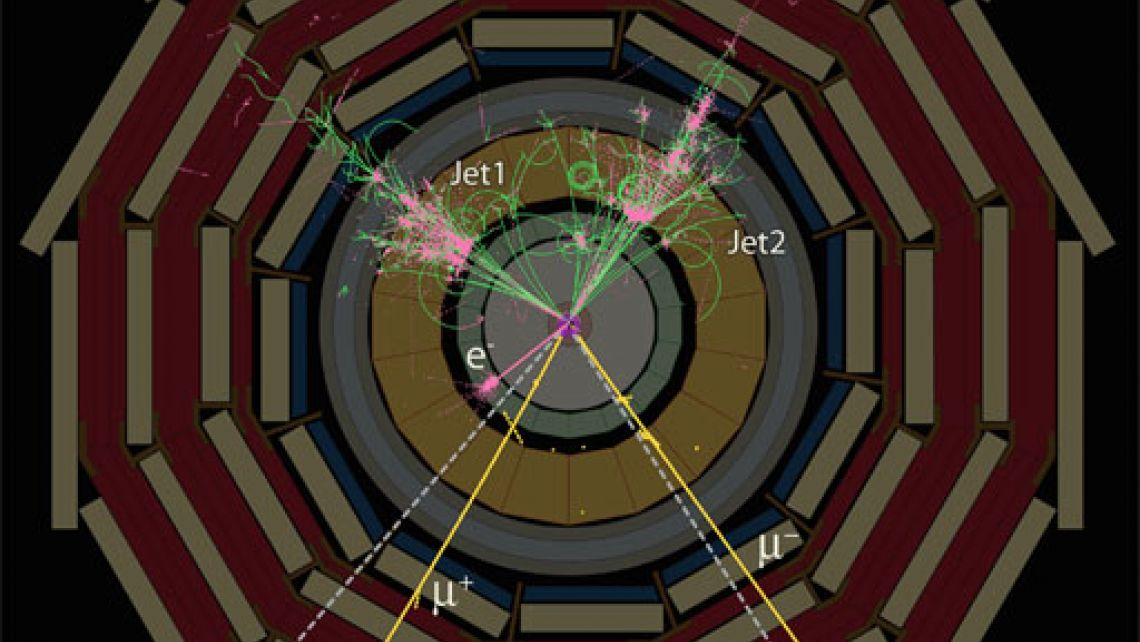
\includegraphics[scale=0.3]{Detector/SusyAny.jpg}
    \caption{This event indicates the formation of  supersymmetric particles. Particle decay  is like requiring an individual CMS layer  to detect the entire range of particles being formed (electrons, muon neutrinos, neutrinos, jets produced by quarks).\cite{CMS_3}}
    \label{fig:my_label_detect}
\end{figure}

\begin{figure}[h]
    \centering
    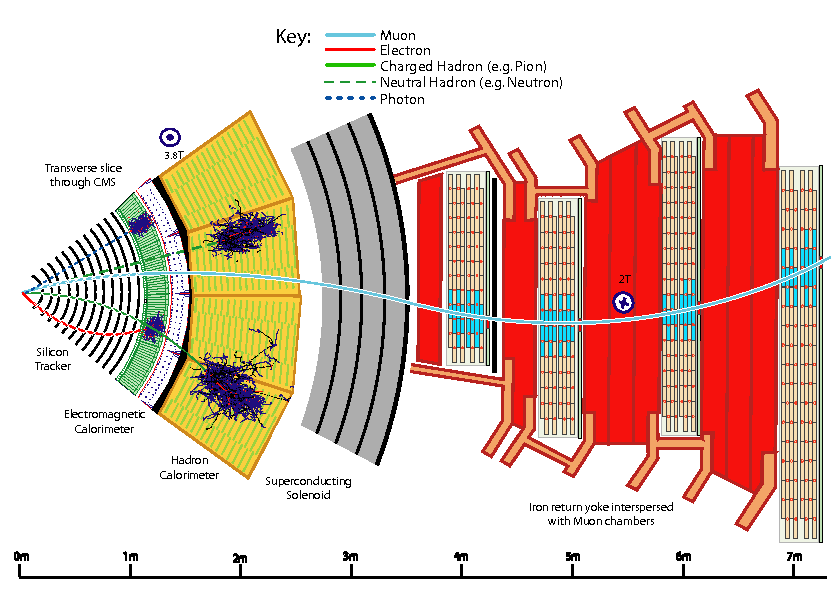
\includegraphics[scale=0.3]{Detector/Figure_001.png}
    \caption{Sketch of the specific particle interactions in a transverse slice of the CMS detector, from the beam interaction region to the muon detector. The muon and the charged pion are positively charged, and the electron is negatively charged\cite{CMS_3}}
    \label{fig:my_label_CMS}
\end{figure}

The main function of CMS:
\begin{itemize}
    \item Bending Particles
    \item Identifying tracks
    \item Measuring energy
    \item Detecting muons
\end{itemize}
There are many other use such as medical imagining and etc.\\
A CMS consists of a layer of detector material that captures and measures the energy or momentum of each particle by taking advantage of the various properties of the particle. New particles found in CMS usually quickly transform into an unstable, lighter, more stable, better-understood cascade of particles.




% \includemovie{1cm}{1cm}{Figures/detectoroverview.gif}
% \includegraphics{Figures/detectoroverview.gif}
A particle which emerges from the collision, travel outwards will first encounter the tracking system, made of silicon pixels and silicon strip detectors\cite{Sirunyan_2021}. This pixels and strip detectors act as a camera. These accurately measure the positions of passing charged particles and allowing physicists to reconstruct their tracks. Charged particles follow spiraling paths in the CMS magnetic field and the curvature of their paths reveal their momenta.\cite{CMS_3}\\
The  next layer of the detector, the so-called calorimeter, measures the energy of the emitted particles. Electrons, photons, and jets (particulate sprays produced by quarks) are all  stopped by a calorimeter so that their energy can be measured. The first calorimeter layer is designed to measure electron and photon energies  with high accuracy. These particles interact electromagnetically and are therefore called an electromagnetic calorimeter (ECAL)\cite{CMS_4}.\\

Particles that interact through the strong force hadron store most of their energy in the next layer, the hadron calorimeter (HCAL). The only known particles that penetrate beyond  HCAL are  weakly interacting particles such as muons and neutrinos. Muons are charged particles and are further tracked by muon chamber detectors. Their momentum is also measured from the curvature of the path of the CMS magnetic field. However, neutrinos are neutral and have little interaction, so they avoid detection. You can determine where those particles were by adding  the momentums of all the detected particles and assigning the lost momentum to the neutrinos.\\

% \section{TRIGGERING AND DATA ACQUISITION}
We need a "trigger" to select  potentially interesting events (such as the Higgs boson) from a larger dataset generated after a proton-proton interaction collision. These triggers help reduce the rate to just a few hundred "events" per second. These events can be sampled and stored on your computer's hard drive for later analysis.\cite{CMS_5}. At the end, We are only left with only the collision events that might teach us something new about physics.\\ 
% When CMS is performing at its peak, about one billion proton-proton interactions will take place every second inside the detector. There is no way that data from all these events could be read out, and even if they could, most would be less likely to reveal new phenomena; they might be low-energy glancing collisions for instance, rather than energetic, head-on interactions.We therefore need a “trigger” that can select the potentially interesting events, such as those which will produce the Higgs particle, and reduce the rate to just a few hundred “events” per second, which can be read out and stored on computer disk for subsequent analysis.\\

% However, with groups of protons colliding 40 million times per second there are only ever 25 nanoseconds (25 billionths of a second) before the next lot arrive. New waves of particles are being generated before those from the last event have even left the detector! The solution is to store the data in pipelines that can retain and process information from many interactions at the same time. To not confuse particles from two different events, the detectors must have very good time resolution and the signals from the millions of electronic channels must be synchronised so that they can all be identified as being from the same event.\\
% Level 1 of the trigger is an extremely fast and wholly automatic process that looks for simple signs of interesting physics, e.g. particles with a large amount of energy or in unusual combinations. This is like a reader simply scanning the headlines of a newspaper to see if anything catches their eye. This way we select the best 100,000 events or “issues” each second from the billion available. For the next test, the higher level trigger, we assimilate and synchronise information from different parts of the detector to recreate the entire event - like collating the different pages to form the full newspaper - and send it to a farm of more than 1000 standard computers.


% \url{https://cms.cern/detector/triggering-and-data-acquisition}


% \section{SILICON STRIPS}
% https://cms.cern/detector/identifying-tracks/silicon-strips
On the way out of the tracker, the particles pass through 10 layers of a 130 cm silicon strip detector. This tracker silicon strip detector consists of four inner  layers (TIBs) assembled into a shell with two internal end caps (TIDs), each with three small discs. The outer barrel (TOB) consists of six concentric layers (see \autoref{fig:my_label_Concentric}). Finally, the two end caps (TECs) close  the tracker. Each has a silicon module designed to be different depending on its position in the detector. This part of the tracker contains 15,200  sensitive modules and a total of 10 million detector strips read by 80,000 microelectronic chips. Each module consists of three elements: sensors, mechanical support structure and electronics. These silicon are very suited to receive many particles in a small space due to their fast response and good spatial resolution. The small amount of charge generated after knocking of electron from atoms get amplified by APV25 chips, allows us to reconstruct its path.
\begin{figure}[H]
    \centering
    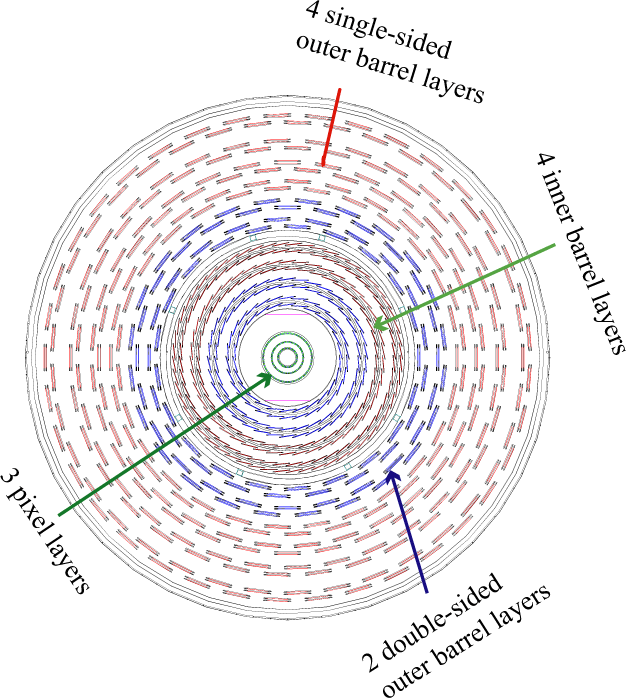
\includegraphics[scale=0.3]{Detector/Barrel.png}
    \caption{CMS Tracker layer shown in perpendicular to the beam\cite{CMS_6}}
    \label{fig:my_label_Concentric}
\end{figure}


% After the pixels and on their way out of the tracker, particles pass through ten layers of silicon strip detectors, reaching out to a radius of 130 centimetres.
% The tracker silicon strip detector consists of four inner barrel (TIB) layers assembled in shells with two inner endcaps (TID), each composed of three small discs. The outer barrel (TOB) consists of six concentric layers. Finally two endcaps (TEC) close off the tracker. Each has silicon modules designed differently for its place within the detector. This part of the tracker contains 15,200 highly sensitive modules with a total of 10 million detector strips read by 80,000.  Each module consists of three elements: a set of sensors, its mechanical support structure and readout electronics. \\
% Silicon sensors are highly suited to receive many particles in a small space due to their fast response and good spatial resolution. microelectronic chips. Each module consists of three elements: a set of sensors, its mechanical support structure and readout electronics. \\
% Silicon sensors are highly suited to receive many particles in a small space due to their fast response and good spatial resolution. The silicon detectors work in much the same way as the pixels: as a charged particle crosses the material it knocks electron from atoms and within the applied electric field these move giving a very small pulse of current lasting a few nanoseconds. This small amount of charge is then amplified by APV25 chips, giving us “hits” when a particle passes, allowing us to reconstruct its path.

% Due to the nature of their job, the tracker and its electronics are pummeled by radiation but they are designed to withstand it. To minimise disorder in the silicon this part of the detector is kept at -20oC, to “freeze” any damage and prevent it from perpetuating.

% The charge on each microstrip is read out and amplified by an Analogue Pipeline Voltage (APV25) chip. Four or six such chips are housed within a “hybrid”, which also contains electronics to monitor key sensor information, such as temperature, and provide timing information in order to match “hits” with collisions. The APV25 stores the signals in a memory for several microseconds and then processes them before sending to a laser to be converted into infrared pulses. These are then transmitted over a 100m fibre optic cable for analysis in a radiation-free environment. The tracker uses 40,000 such fibre optic links providing a low power, lightweight way of transporting the signal. Much of the technology behind the tracker electronics came from innovation in collaboration with industry. \\
% \section{SILICON PIXELS}

% https://cms.cern/detector/identifying-tracks/silicon-pixels

% \section{TRACKING}
% https://cms.cern/detector/identifying-tracks

% The pixel detector, though about the size of a shoebox, contains 65 million pixels, allowing it to track the paths of particles emerging from the collision with extreme accuracy. Each layer is spilt into segments like tiny kitchen tiles, each a little silicon sensor, 100µm by 150µm, about two hairs widths. When a charged particle passes through it gives enough energy for electrons to be ejected from the silicon atoms, creating electron-hole pairs. Each pixel uses an electric current to collect these charges on the surface as a small electric signal. A electronic silicon chip, one for each tile is attached, using an almost microscopic spot of solder using the so-called bump bonding technique, which amplifies the signal.Knowing which pixels have been touched allows us to deduce the particle's trajectory. And because the detector is made of 2D tiles, rather than strips, and has a number of layers, we can create a three-dimensional picture. Because there are 65 million channels, the power for each pixel must be kept to a minimum. Even with each only generating around 50 microwatts, the total power output is around the same as the energy produced by a hot plate. So as not to overheat the detector, the pixels are mounted on cooling tubes.\\
% % \section{MEASURING ENERGY}
% https://cms.cern/detector/measuring-energy
Electromagnetic calorimeters (ECALs) are two inner layers that measure their energy by completely stopping electrons and photons. Hadrons, a composite particle of quarks and gluons, pass through the ECAL and are blocked by an outer layer called the hadron calorimeter (HCAL). A photodetector specifically designed to work in high magnetic fields is also glued to the back of each crystal to capture scintillation light and convert it into an electrical signal.
 
% \section{ENERGY OF ELECTRONS AND PHOTONS (ECAL)}
% https://cms.cern/detector/measuring-energy/energy-electrons-and-photons-ecal\\
% CMS must find the energies of emerging particles. Of particular interest are electrons and photons, because of their use in finding the Higgs boson and other new physics.

% The particles are measured using an electromagnetic calorimeter (ECAL). But to find them with the necessary precision in the very strict conditions of the LHC - a high magnetic field, high levels of radiation and only 25 nanoseconds between collisions - required very particular detector materials.\\ 
% Lead tungstate crystal is made primarily of metal and is heavier than stainless steel, but with a touch of oxygen in this crystalline form it is highly transparent and “ scintillates ” when electrons and photons pass through it. This means it produces light in proportion to the particle’s energy. These high-density crystals produce light in fast, short, well-defined photon bursts that allow for a precise, fast and fairly compact detector.

% Photodetectors that have been especially designed to work within the high magnetic field, are also glued onto the back of each of the crystals to detect the scintillation light and convert it to an electrical signal that is amplified and sent for analysis.

% The ECAL, made up of a barrel section and two ”endcaps”, forms a layer between the tracker and the HCAL. The cylindrical “barrel” consists of 61,200 crystals formed into 36 “supermodules”, each weighing around three tonnes and containing 1700 crystals. The flat ECAL endcaps seal off the barrel at either end and are made up of almost 15,000 further crystals.

% For extra spatial precision, the ECAL also contains Preshower detectors that sit in front of the endcaps. These allow CMS to distinguish between single high-energy photons (often signs of exciting physics) and the less interesting close pairs of low-energy photons.
% The CMS ECAL…

% crystals each weigh 1.5kg but with a volume roughly equal to that of a small coffee cup,
% contains nearly 80,000 such crystals, each of which took two days to grow.

% https://cms.cern/detector/measuring-energy/energy-hadrons-hcal\\

% https://cms.cern/detector/detecting-muons\\
% https://cms.cern/detector/computing-grid\\
To meet this challenge, the vast amount of data obtained from the CMS needs to be analyzed, and LHC has adopted a new computing system, a distributed computing and data storage infrastructure called the Worldwide LHC Computing Grid (WLCG). doing. The grid works together with tens of thousands of standard PCs around the world to provide far more processing power than  a single supercomputer can achieve, giving  thousands of scientists around the world access to data. \cite{CMS_7}.

% The “Tier 0” centre at CERN first reconstructs the full collision events and analysts start to look for patterns; but the data has a long way to go yet. Once CERN has made a primary backup of the data it is then sent to large “Tier 1” computer centres in seven locations around the world: in France, Germany, Italy, Spain, Taiwan, the UK and the US. Here events are reconstructed again, using information from the experiment to improve calculations using refined calibration constants.

% Tier 1 starts to interpret and make sense of the particle events and collate the results to see patterns emerging. Meanwhile each sends the most complex events to a number of “Tier 2” facilities, which total around 40, for further specific analysis tasks. In this way information braches out from each tier across the world so that, on a local level.
% , physicists and students whether in Rio de Janeiro or Oxford, can study CMS data from their own computer, updated on a regular basis by the LHC Computing Grid.
 Charged particle trajectories are measured by the silicon pixel and strip sub detectors\cite{Palichik:2018wwn}, covering 0 <$\phi$ <2$\pi$ in azimuth and $|\eta|$ < 2.5, where the pseudo rapidity $\eta$ is defined as 
 \begin{equation*}
     \eta = -ln[\tan \theta/2],
 \end{equation*}
 
 with $\theta$ being the polar angle of the trajectory of the particle with respect to the counterclockwise-beam direction. Within the field
volume, the silicon detectors are surrounded by a crystal electromagnetic calorimeter and a brass/scintillator hadron calorimeter that provide high resolution energy measurement of photons, electrons and hadronic jets.



% \textbf{Complte this part in 1500- 2000 words}
% The Compact Muon Solenoid (CMS) is a particle detector built to study pp collisions at the LHC.
% The detector has a diameter of 15 m and a length of 21.6 m. The key feature of the detector is
% its large superconducting solenoid with an internal diameter of 6m that creates a magnetic field
% of 3.8 T. The magnetic field helps to bend the trajectories of charged particles in order to identify
% their momentum and charge. Fig 1.3 shows a transverse view of the detector.
% The detector is built hermetically around the beam pipe (where pp collisions take place) and has
% several different modules specialized in identifying certain types of particles. Closest to the beam
% pipe are the silicon pixel and strip detectors, which help in identifying charged particle tracks.
% Surrounding this is the Electromagnetic Calorimeter (ECAL), which is made up of scintillating
% lead-tungstate crystals and helps to identify energy deposits from photons and electrons. The
% Hadron Calorimeter (HCAL) is a sampling calorimeter built from brass and a scintillator and helps
% to identify energy deposits from charged and neutral hadrons. The pixel and strip trackers, ECAL
% and the HCAL are enclosed within the solenoid (magnetic) volume. Outside the magnet are the
% muon chambers which are gas ionization chambers and are used to identify muons. These muon
% chambers are embedded in steel return yokes of the magnet. Muons can travel several metres
% without interacting. This is the reason why muon detectors are placed at the outer edge of the



% About LHC
% The Large Hadron Collider (LHC) is the world’s largest and most powerful particle accelerator. The LHC consists of a 27-kilometer ring of superconducting magnets with a number of accelerating structures to boost the energy of the particles along the way. Inside the accelerator, two high-energy particle beams travel at close to the speed of light before they are made to collide. The beams travel in opposite directions in separate beam pipes – two tubes kept at ultrahigh vacuum. They are guided around the accelerator ring by a strong magnetic field maintained by superconducting electromagnets. The electromagnets are built from coils of special electric cable that operates in a superconducting state, efficiently conducting electricity without resistance or loss of energy. This requires chilling the magnets to ‑271.3°C. For this reason, much of the accelerator is connected to a distribution system of liquid helium, which cools the magnets, as well as to other supply services. Thousands of magnets of different varieties and sizes are used to direct the beams around the accelerator. These include 1232 dipole magnets 15 metres in length which bend the beams, and 392 quadrupole magnets, each 5–7 metres long, which focus the beams. 
% protons for beams in 27-kilometre ring come from a single bottle of hydrogen gas, replaced only twice per year to ensure that it is running at the correct pressure.
% How to accelerate protons
% In the first part of the accelerator, an electric field strips hydrogen atoms (consisting of one proton and one electron) of their electrons. Electric fields along the accelerator switch from positive to negative at a given frequency, pulling charged particles forwards along the accelerator. CERN engineers control the frequency of the change to ensure the particles accelerate not in a continuous stream, but in closely spaced “bunches”.

% Radiofrequency (RF) cavities
% These are specially designed metallic chambers, spaced at intervals along the accelerator – are shaped to resonate at specific frequencies, allowing radio waves to interact with passing particle bunches. Each time a beam passes the electric field in an RF cavity, some of the energy from the radio waves is transferred to the particles, nudging them forwards.It’s important that the particles do not collide with gas molecules on their journey through the accelerator, so the beam is contained in an ultrahigh vacuum inside a metal pipe – the beam pipe.

% Various types of magnet
% These serve different functions around a circular accelerator. Dipole magnets, for example, bend the path of a beam of particles that would otherwise travel in a straight line. The more energy a particle has, the greater the magnetic field needed to bend its path. Quadrupole magnets act likes lenses to focus a beam, gathering the particles closer together. 


% Energies Units 
% Energy has many units in physics: joules, calories, and kilowatt hours are all units of energy used in different contexts. Only the joule is an International System (SI) unit, but all of them are related by conversion factors. In particle physics, the unit that is most frequently used for energy is the electronvolt (eV) and its derivatives keV (10^3 eV), MeV (10^6 eV), GeV (10^9 eV) and TeV (10^12 eV). The electronvolt is a convenient unit because, in absolute terms, the energies that particle physicists deal with are very small. If we take the LHC as an example, the design value of the total collision energy is 14 TeV

% The definition of the electronvolt comes from the simple insight that a single electron accelerated by a potential difference of 1 volt will have a discrete amount of energy (measured in joules), E=qV where q is the charge on the electron in coulombs and V is the potential difference in volts. Hence 1 eV = (1.602 x 10–19 C) x (1 V) = 1.602 x 10–19 J.

% What is an accelerator?
% An accelerator propels charged particles, such as protons or electrons, at high speeds, close to the speed of light. They are then smashed either onto a target or against other particles circulating in the opposite direction. By studying these collisions, physicists are able to probe the world of the infinitely small.

 
% The Large Hadron Collider is the most powerful accelerator in the world. It boosts particles, such as protons, which form all the matter we know. Accelerated to a speed close to that of light, they collide with other protons. These collisions produce massive particles, such as the Higgs boson or the top quark. By measuring their properties, scientists increase our understanding of matter and of the origins of the Universe. These massive particles only last in the blink of an eye, and cannot be observed directly. Almost immediately they transform (or decay) into lighter particles, which in turn also decay. The particles emerging from the successive links in this decay chain are identified in the layers of the detector.



% How an accelerator works
% Their job is to speed up and increase the energy of a beam of particles by generating electric fields that accelerate the particles, and magnetic fields that steer and focus them. 
% Accelerators use electromagnetic fields to accelerate and steer particles. Radiofrequency cavities boost the particle beams, while magnets focus the beams and bend their trajectory.
% In a circular accelerator, the particles repeat the same circuit for as long as necessary, getting an energy boost at each turn. In theory, the energy could be increased over and over again. However, the more energy the particles have, the more powerful the magnetic fields have to be to keep them in their circular orbit.
% A linear accelerator, on the contrary, is exclusively formed of accelerating structures since the particles do not need to be deflected, but they only benefit from a single acceleration pass. In this case, increasing the energy means increasing the length of the accelerator.
% As physicists have been explored higher and higher energies, accelerators have become larger and larger: the size of an accelerator is a compromise between energy, the radius of curvature (if it’s circular), the feasibility and the cost.
% Colliders are accelerators that generate head-on collisions between particles. Thanks to this technique, the collision energy is higher because the energy of the two particles is added together.
% The Large Hadron Collider is the largest and most powerful collider in the world. It boosts the particles in a loop 27 kilometres in circumference at an energy of 6.5 TeV (teraelectronvolts), generating collisions at an energy of 13 TeV.
% What are the characteristics of an accelerator?
% The type of particles, the energy of the collisions and the luminosity are among the important characteristics of an accelerator. An accelerator can circulate a lot of different particles, provided that they have an electric charge so that they can be accelerated with an electromagnetic field. The CERN accelerator complex accelerates protons, but also nuclei of ionized atoms (ions), such as the nuclei of lead, argon or xenon atoms. Some LHC runs are thus dedicated to lead-ion collisions. The ISOLDE facility accelerates beams of exotic nuclei for nuclear physics studies. The energy of a particle is measured in electronvolts. One electronvolt is the energy gained by an electron that accelerates through a one-volt electrical field. As they race around the LHC, the protons acquire an energy of 6.5 million million electronvolts, known as 6.5 tera-electronvolts or TeV. It is the highest energy reached by an accelerator, but in everyday terms, this is a ridiculously tiny energy; roughly the energy of a safety pin dropped from a height of just two centimetres. But an accelerator concentrates that energy at the infinitesimal scale to obtain very high concentrations of energy close to those that existed just after the Big Bang.
% Luminosity is a key indicator of an accelerator’s performance: it indicates the number of potential collisions per surface unit over a given period of time. The instantaneous luminosity is expressed in cm-2s-1 and the integrated luminosity, corresponding to the number of collisions that can occur over a given period, is measured in inverse femtobarn. One inverse femtobarn corresponds to 100 million millions (potential) collisions.
% What type of accelerators are at CERN?
% CERN operates a complex of eight accelerators and two decelerators. These accelerators supply experiments or are used as injectors, accelerating particles for larger accelerators. Some, such as the Proton Synchrotron (PS) or Super Proton Synchrotron (SPS) do both at once, preparing particles for experiments that they supply directly and injecting into larger accelerators.
% The Large Hadron Collider is supplied with protons by a chain of four accelerators that boost the particles and divide them into bunches.
 
% CERN’s accelerator complex

% The accelerator complex at CERN is a succession of machines that accelerate particles to increasingly higher energies. Each machine boosts the energy of a beam of particles before injecting it into the next machine in the sequence. In the Large Hadron Collider (LHC) – the last element in this chain – particle beams are accelerated up to the record energy of 6.5 TeV per beam.
 
% Linear accelerator 4 (Linac4) became the source of proton beams for the CERN accelerator complex in 2020. It accelerates negative hydrogen ions (H-, consisting of a hydrogen atom with an additional electron) to 160 MeV to prepare them to enter the Proton Synchrotron Booster (PSB). The ions are stripped of their two electrons during injection from Linac4 into the PSB, leaving only protons. These are accelerated to 2 GeV for injection into the Proton Synchrotron (PS), which pushes the beam up to 26 GeV. Protons are then sent to the Super Proton Synchrotron (SPS), where they are accelerated up to 450 GeV.

% The protons are finally transferred to the two beam pipes of the LHC. The beam in one pipe circulates clockwise while the beam in the other pipe circulates anticlockwise. It takes 4 minutes and 20 seconds to fill each LHC ring, and 20 minutes for the protons to reach their maximum energy of 6.5 TeV. Beams circulate for many hours inside the LHC beam pipes under normal operating conditions. The two beams are brought into collision inside four detectors – ALICE, ATLAS, CMS and LHCb – where the total energy at the collision point is equal to 13 TeV.
% Protons are not the only particles accelerated in the LHC. Lead ions for the LHC start from a source of vaporised lead and enter Linac3 before being collected and accelerated in the Low Energy Ion Ring (LEIR). They then follow the same route to maximum energy as the protons.


% Luminosity gives a measure of how many collisions are happening in a particle accelerator, so why don’t we just say collision rate?
% Luminosity gives a measure of how many collisions are happening in a particle accelerator, so we’re often asked why we don’t just say collision rate. It’s a very reasonable question. The answer is because luminosity isn’t strictly speaking the collision rate: it measures how many particles we’re able to squeeze through a given space in a given time. That doesn’t mean that those particles will all collide, but the more we can squeeze into a given space, the more likely they are to collide.
% The best place to start is with what physicists refer to as a cross-section. Usually, a cross-section is a measure of the size of something. For example, a barn door has a bigger cross-section – it covers a larger area – than a cat flap. In particle physics, a cross-section is a measure of the probability of something happening, and it’s measured in units called…. barns. In reality, a barn is a huge cross-section and most processes have cross-sections measured in tiny fractions of a barn.
% When protons collide in the LHC, many things can happen: the protons can just glance off each other, or they can collide more violently producing any of a range of new particles. Each of these processes has its own cross-section. The cross-section for the production of a Higgs particle, for example, is very small at the scale of nanobarns – billionths of a barn  – which means that Higgs particles, if they exist, will be produced very rarely.
% When looking for something that rare, the more collisions you have, the more likely it is that the rare thing will happen, and that’s why particle physicists care so much about luminosity. It works a bit like this: if you multiply the luminosity of the beam by the cross-section for any process, such as Higgs production, you get the rate at which you can expect that process to happen. If you multiply the luminosity by the sum of the cross-sections for all possible processes, you get the total number of collisions.
% To help figure out the different ways that luminosity contributes to the collision rate, think of rolling marbles from opposite ends of a corridor. If you’ve just got one person at each end of the corridor, the chances they’ll get their marbles to collide are small: the luminosity is pretty low. But put lots of people at each end and the luminosity goes up. Similarly, if you increase the cross-section by rolling footballs down the corridor, the luminosity remains the same, but since a football has a bigger cross-section than a marble, the number of collisions goes up. It’s not a perfect analogy, but I hope you get the idea.
% The LHC’s design luminosity is 1034 per square centimetre per second. That’s a big number, and although we can’t say exactly how many collisions it equates to, we can say that and it’s around 600 million collisions per second on average. When the LHC run ended in 2010, the luminosity was around 2×1032 per square centimetre per second, giving a few million proton collisions per second.
% The other way that physicists use luminosity is to add it all up, or integrate it. If you do that, you get a measure of the total number of collisions that have happened. So, for example, the integrated luminosity recorded by the ATLAS and CMS experiments in 2010 was around 45 inverse picobarns, which translates to over 3000 billion collisions recorded.  And what about the Higgs particle? With the peak luminosity reached by the LHC last year, we might have expected Higgs particles to be produced at the rate of a handful a day, which is not yet enough for us to see a signal above the background from known and well-understood physics. To claim a discovery, physicists need to see a statistically significant excess over and above what they expect to see from known physics, and they measure the degree of significance using a quantity called a standard deviation, or sigma for short
% Restarting the LHC: Why 13 Tev?
% The LHC was designed to run at a maximum collision energy of 14 TeV, so why has CERN decided to start the second run at a lower energy?
% The Large Hadron Collider (LHC) is scheduled to restart for physics early in 2015 after two years of maintenance and upgrading. The collision energy at restart will be 13 TeV, a significant increase over the initial three-year LHC run, which began with a collision energy of 7 TeV, rising to 8 TeV. But the LHC was designed to run at a maximum collision energy of 14 TeV, so why has CERN decided to start the second run at a lower energy?
% The decision to begin the LHC’s second run at 13 TeV has been taken in order to optimise the delivery of particle collisions for physics research, and thereby speed the route to potential new physics. It is based on the properties of the 1232 superconducting dipole magnets that guide the beams around the LHC’s 27-kilometre ring. The higher the beam energy, the higher the magnetic field needed to maintain a constant orbit, and the higher the electric current flowing in the magnet’s superconducting coils.
% At LHC beam energies, the electric currents are extremely high, up to 12,000 Amperes, and superconducting cables have to be used. Superconductivity is a low-temperature phenomenon, so the coils have to be kept very cold, just 1.9 degrees above absolute zero to be precise, or about -271°C. Even a tiny amount of energy released into the magnet for any reason can warm the coils up, stopping them from superconducting. When this happens, the current has to be safely extracted in a very short time. This is called a quench, and just one millijoule – the energy deposited by a 1-centime euro coin falling from 5 cm – is enough to provoke one. Magnet protection in case of quenches is a crucial part of the design of the LHC’s magnetic system.  
% When a new superconducting magnet is qualified for use, it needs to be trained. That involves steadily increasing the current until the magnet quenches, then starting again. At first, the quenches may occur at relatively low current, but over time, as the components of the magnet settle in, the current increases until the magnet can be operated routinely at its nominal current. If a new training cycle is started after an extended period during which the magnet is warm, the magnet usually restarts training at a value that is higher than first quench in the first training cycle but lower than the maximum previously reached. In other words, the magnet’s ‘memory’ is usually less than 100%.
% Before the LHC started operation, all of its magnets were trained up to a current equivalent to a collision energy of over 14 TeV. Tests with individual magnets, along with hardware commissioning tests in 2008, have shown that for some dipole magnets the memory is slightly lower than expected, demanding a larger number of quenches to reach nominal field. However, retraining these magnets to 13 TeV should require only a short period of time, whereas retraining to 14 TeV would take longer, taking time away from physics research. That’s why the best way to get to new results quickly, at an energy considerably higher than ever achieved before, is to start operation at 13 TeV. A decision on when to go higher will be taken at a later date in the LHC’s second run..
 
% Interesting:
% https://home.cern/science/accelerators/accelerator-complex/panoramas
% Accelerating: Radiofrequency cavities
% To accelerate particles, the accelerators are fitted with metallic chambers containing an electromagnetic field known as radiofrequency (RF) cavities. Charged particles injected into this field receive an electrical impulse that accelerates them. In the Large Hadron Collider (LHC), 16 RF cavities are housed in four cylindrical refrigerators called cryomodules, which enable them to work in a superconducting state. Each cavity is driven by a high-power klystron, which is a tube containing electron beams. The electron beams are intensity-modulated to a frequency of 400 MHz, or 400 million oscillations per second. A rectangular pipe of conducting metal called a waveguide directs energy to the cavity. The cavity’s shape has been specifically designed to achieve resonance and the build up in intensity of the electromagnetic waves. Each cavity can reach a maximum voltage of 2 megavolts (MV), corresponding to 16 MV per beam. The LHC’s RF cavities bring the 450 GeV energy of the particles (1 GeV = 1 billion electronvolts) to 6.5 TeV (1 TeV = 1 million million electronvolts) - more than 14 times their injection energy. The maximum energy is reached in around 20 minutes with the bunches having passed through the RF cavities more than 10 million times. The field in an RF cavity is made to oscillate (switch direction) at a given frequency, so timing the arrival of particles is important. In the LHC, each RF cavity is tuned to oscillate at 400 MHz. When the beam has reached the required energy, an ideally timed proton with exactly the right energy will not be accelerated. By contrast, protons with slightly different energies arriving earlier or later will be accelerated or decelerated so that they stay close to the desired energy. In this way, the particle beam is sorted into packs of protons called "bunches". Aside from these accelerating cavities, CERN is developing “crab” cavities for the LHC’s successor, the High-Luminosity LHC. The purpose of these crab cavities is to give a transverse momentum to steer the particles as they approach the collision point.
% How a detector works
% Accelerators at CERN boost particles to high energies before they are made to collide inside detectors. The detectors gather clues about the particles – including their speed, mass and charge – from which physicists can work out a particle's identity. The process requires accelerators, powerful electromagnets, and layer upon layer of complex subdetectors.
% Particles produced in collisions normally travel in straight lines, but in the presence of a magnetic field their paths become curved. Electromagnets around particle detectors generate magnetic fields to exploit this effect. Physicists can calculate the momentum of a particle – a clue to its identity – from the curvature of its path: particles with high momentum travel in almost straight lines, whereas those with very low momentum move forward in tight spirals inside the detector.
% Modern particle detectors consist of layers of subdetectors, each designed to look for particular properties, or specific types of particle. Tracking devices reveal the path of a particle; calorimeters stop, absorb and measure a particle’s energy; and particle-identification detectors use a range of techniques to pin down a particle's identity.
% Tracking devices
% Tracking devices reveal the paths of electrically charged particles as they pass through and interact with suitable substances. Most tracking devices do not make particle tracks directly visible, but record tiny electrical signals that particles trigger as they move through the device. A computer program then reconstructs the recorded patterns of tracks.
% One type of particle, the muon, interacts very little with matter – it can travel through metres of dense material before being stopped. Muons, therefore, pass easily through the inner layers of a detector, which is why muon chambers – tracking devices specialized in detecting muons – usually make up the outermost layer of a detector.

% Calorimeters
% A calorimeter measures the energy a particle loses as it passes through. It is usually designed to stop entirely or “absorb” most of the particles coming from a collision, forcing them to deposit all of their energy within the detector, thus measuring their full energy. Calorimeters have to perform two different tasks at the same time – stopping particles and measuring energy loss – so they usually consist of layers of different materials: a “passive” or “absorbing” high-density material – for example, lead – interleaved with an “active” medium such as plastic scintillators or liquid argon.
% Electromagnetic calorimeters measure the energy of electrons and photons as they interact with the electrically charged particles in matter. Hadronic calorimeters sample the energy of hadrons (particles containing quarks, such as protons and neutrons) as they interact with atomic nuclei. Calorimeters can stop most known particles except muons and neutrinos.

% Particle-identification detectors
% In addition to measuring a particle's momentum in tracking devices and its energy in calorimeters, physicists have further methods of narrowing down its identity. These methods all rely on measuring a particle's velocity, since this, in combination with the momentum measured in the tracking devices, helps to calculate a particle's mass and therefore its identity.
% Velocity can be measured using several methods. The simplest is to measure how much time it takes for a particle to travel a certain distance, using precise time-of-flight detectors. Another method looks at how much a particle ionises the matter that it passes through, as this is velocity-dependent and can be measured by tracking devices.
% If a charged particle travels faster than light through a given medium, it emits Cherenkov radiation at an angle that depends on its velocity. Alternatively, when a particle crosses the boundary between two electrical insulators with different resistances to electric currents, it emits transition radiation, the energy of which depends on the particle's velocity.
% Collating all these clues from different parts of the detector, physicists build up a snapshot of what was in the detector at the moment of a collision. The next step is to scour the collisions for unusual particles, or for results that do not fit current theories.
% Insertion magnets
% When the particle beams enter the detectors, insertion magnets take over. Particles must be squeezed closer together before they enter a detector so that they collide with particles coming from the opposite direction. Three quadrupoles are used to create a system called an inner triplet. There are eight inner triplets, two of which are located at each of the four large LHC detectors, ALICE, ATLAS, CMS and LHCb. Inner triplets tighten the beam, making it 12.5 times narrower – from 0.2 millimetres down to 16 micrometres across.
% After the beams collide in the detector, enormous magnets aid the measurement of particles. For example, physicists look at how charged particles bend in the magnetic field to determine their identity. Charged particles are deflected by the magnetic field in the detector, and their momentum can be calculated from the amount of deflection.
% After colliding, the particle beams are separated again by dipole magnets. Other magnets minimize the spread of the particles from the collisions. When it is time to dispose of the particles, they are deflected from the LHC along a straight line towards the beam dump. A "dilution" magnet reduces the beam intensity by a factor of 100,000 before the beam collides with a block of concrete and graphite composite for its final stop.
% Insertion magnets are also responsible for beam cleaning, which ensures that stray particles do not come in contact with the LHC’s most sensitive components.
\setcounter{equation}{0}
\setcounter{table}{0}
\setcounter{figure}{0}
%\baselineskip 24pt


    



\clearpage
\afterpage{\blankpage}
\chapter{\label{ML}Machine Learning}
% \epigraph{Machine Learning can be defined as the process of inducing intelligence into a system or machine without explicit programming}{-Andrew NG}

Machine learning (ML) is a common term used to describe all automated reasoning techniques in the broadest sense. Therefore, machine learning plays an important role in almost every area of high energy physics. Traditionally, machine learning has been synonymous with "multivariate technology."  Boosted decision trees as a community favorite method and TMVA  as a community favorite tool. The set of methods and tools commonly used in HEP has grown significantly in recent years\cite{https://doi.org/10.48550/arxiv.2102.02770}. \\
Machine learning techniques are designed to leverage large datasets  to reduce complexity and discover new features in the data. The  most commonly used machine learning algorithms in HEP today are Boosted Decision Trees (BDT) and Neural Networks (NN). Variables related to physical problems are typically selected and  machine learning models are trained  using signal and background events for classification or regression (for example). Model training is the most human and CPU-time-consuming step, but the application called the  inference phase is relatively inexpensive. BDT and NN are typically used to classify particles and events. These are also used for regression. In regression, for example, a continuous function is trained to get the best estimate of the energy of a particle based on. 
 Measurements from several detectors.Neural networks have been used in HEP ​​for some time; however, improvements in training algorithms and computing power have led to the so-called deep learning revolution over the last decade, which has had a major impact on HEP\cite{https://doi.org/10.48550/arxiv.2102.02770}. Deep learning is especially promising when there is a large amount of data and functionality, and there are symmetries and complex nonlinear dependencies between inputs and outputs. There are different types of DNNs used in HEP: Full Connection (FCN), Convolution (CNN), and Recurrent (RNN). In addition, neural networks are used in the context of generative models, and neural networks are trained to reproduce the multidimensional distribution of a set of training instances. Variational Autoencoders (VAEs) and the new Generative Adversarial Network (GAN) are two examples of such generative models used in HEP.\\

Numerous machine learning algorithms are dedicated to time series analysis and prediction. If the events are independent of each other, they are usually unrelated to HEP data analysis\cite{https://doi.org/10.48550/arxiv.2008.00444,Ismail_Fawaz_2019}. However, there is growing interest in these algorithms for data quality monitoring, computing and accelerator infrastructure, physical processes, and event reconstruction tasks where time is an important factor\cite{Alzubaidi2021}. 
 This chapter describes the basic concepts of machine learning and how neural networks work, which is more efficient and productive than traditional workflows.



\section{Types of Machine Learning:}
There are four basic approaches for machine learning: supervised learning, unsupervised learning, semi-supervised learning, and reinforcement learning\cite{Sarker2021}. The type of algorithm that will be used depends on what type of data they want to predict.

\subsection{Supervised Learning}
In this type of machine learning, we supply algorithms with labeled training datasets and define the variables that we want the algorithm to assess for correlations and the outputs. 
Both the input and the output of the algorithm have been already specified. Supervised machine learning requires getting trained with the algorithm on both labeled inputs and desired outputs. A simple example would be the classification of datasets\cite{https://doi.org/10.48550/arxiv.2003.05199}.

\subsection{Unsupervised learning:}
This type of machine learning involves algorithms that train on unlabeled datasets. The algorithm scans through datasets looking for any meaningful connection without any human intervention. The data on which algorithms train as well as the predict the output is predetermined. For example, unsupervised learning is used for Google news categorization, visual perception tasks such as image recognition, anomaly detection, classifying customers, etc\cite{Ghahramani2004}.

\subsection{Semi-supervised learning:}
This approach to machine learning involves a mix of both the previous types of the dataset; that is algorithm is trained upon the combination of the labeled and unlabeled dataset.  In this type of algorithm, the programmer just needs to cluster similar data using an unsupervised learning algorithm and further use the existing labeled data to label the rest of the unlabeled data. A few practical examples of this type of learning are speech analysis, internet content classifications, and protein sequence classification\cite{Shental05semi-supervisedlearning}.


\subsection{Reinforcement learning: }
Data scientists usually use reinforcement learning to teach a machine to complete a multistep process( based on the rewarding behaviors/ or pushing the undesired one ) for which there is a clearly defined set of rules. In the reinforcement learning decision is dependent on the output of the previous input sequence, so we provide labels to sequences of dependent decisions. For example, chess games or a sitting cat, the cat will only get food when she starts to walk\cite{Thrun92efficientexploration}.\\

A brief summary of how machine learning consists can be summarized from this tree diagram,
% \textbf{Add examples to each of the learning}
\resizebox{\linewidth}{!}{%
\begin{center}
    \begin{forest}
  [Machine Learning
    [Supervised \\ Learning
     [Classification 
       [Binary \\ classification]
       [Multi \\classification]
     ]
     [Regression
       [Regression \\ modeling
         [\textit{Ensembling}]
       ]
     ]
    ]
    [Unsupervised \\ Learning
      [Clustering
      [K-means Clustering]
      ]
      [Anomaly detection
        % [V$'$
        %   [V
        %     [\textit{is}]
        %   ]
        %   [AP
        %     [Deg
        %       [\textit{extremely}]
        %     ]
        %     [A$'$
        %       [A
        %         [\textit{straightforward}]
        %       ]
        %       [CP
        %         [\textit{to wield}, roof]
        %       ]
        %     ]
        %   ]
        % ]
      ]
    ]
    [semi-supervised\\ learning
    ]
    [reinforcement \\learning
    ]
  ]
\end{forest}
\end{center}
}%

\section{Evaluating models}
In machine learning, the ultimate goal is to achieve models that generalize, i.e., that perform well on never-before-seen data, and over fitting is the central obstacle. To do this, splitting the available data is very crucial. Training, validation, and testing are the partitions  
needed, so during the training phase, the model trains with the training data and test with the validation data, and when the model is ready, it is tested one last time with the test data, briefly explained by \autoref{fig:my_label_09876} \\
\begin{figure}[H]
    \centering
    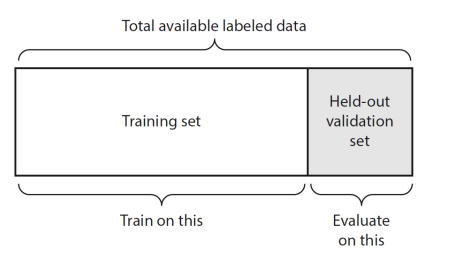
\includegraphics[scale=0.6]{Figure/ml__12.png}
    \caption{Splitting data to be used in the training phase. Image source: [Chollet, 2017]}
    \label{fig:my_label_09876}
\end{figure}
The reason why three (and not two) datasets are used is that tuning in the model configuration is required. The parameters that can be tuned in a machine learning model are called hyperparameters\cite{https://doi.org/10.48550/arxiv.1904.11829,https://doi.org/10.48550/arxiv.1412.3555}. Hyperparameter values can be changed to control the learning process. Meanwhile, the value of other parameters, like node weights, are derived by training and cannot be adjusted. Hyperparameter tuning is done with the feedback of the model performance in the validation data and further applied under an unseen test dataset. This is a basic approach for each machine learning model, and we will apply the same over the neural network model in the next section.

%%%%%%%%%%%%%%%%%%%%%%%%%%%%%%%%%%%%%%%%%%%%%%%%%%%%%%DNNNNNNNNNNNNNDNNNDNNNDNNNNDNNDNNNDNNDNDNNDNDNNDNDNNNDNNNNDNNNDNDNDNDNDNDNDNDNDNDNNDNDNDNDNNDND
\section{Deep Neural Network}
Machine learning works very efficiently on numerous problems but sometimes fails to excel in a few specific cases, which appears very easy for humans. For example, classifying an image as a cat or dog or distinguishing audio clips as a male or female voice,etc\dots The machine fails to identify this type of problem of image classification or video segregation and other unstructured data types, which are easy for us. There come to the idea of a deep neural network(DNN), where the idea is to mimic the human brain's biological process, which is composed of billions of neurons connected to each other and to adapt and learn new things\cite{LeCun2015}. \\ 


A simplified version of Deep Neural Network can be represented as a hierarchical (layered) structure of neurons (compared with the neurons in the human brain) with connections to other neurons. These neurons pass a message or signal to other neurons based on the received input and form a complex network system that learns with some feedback mechanism. The following diagram(\autoref{fig:my_label_hu}) represents an 'N' layered Deep Neural Network.\\

\begin{figure}[H]
    \centering
    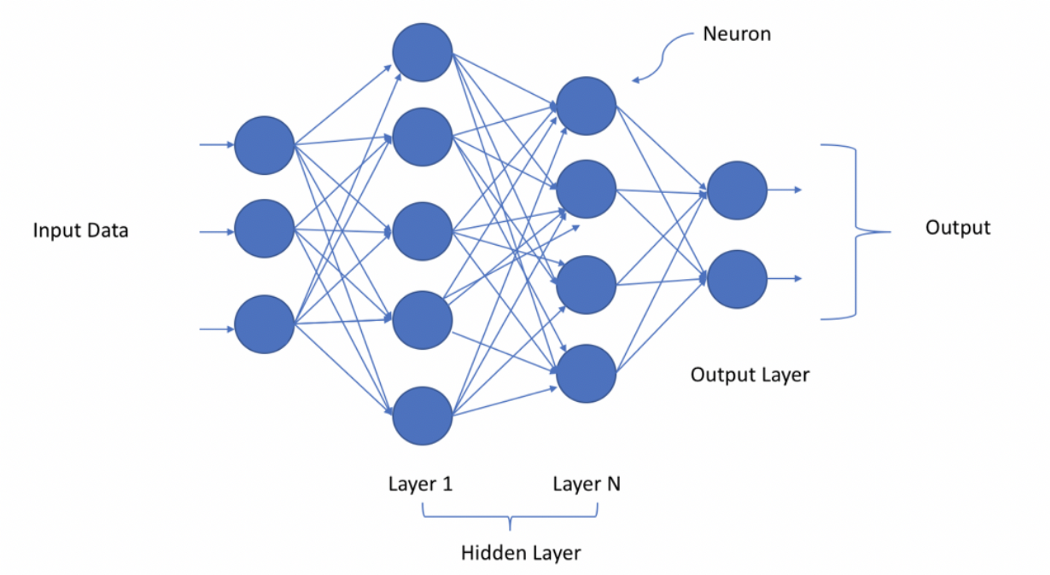
\includegraphics[scale=0.4]{Figure/1_ML_report.png}
    \caption{A Deep Neural Network with N hidden layers}
    \label{fig:my_label_hu}
\end{figure}
The input data is provided to the neurons into the first layer (not hidden), which subsequently provides an output to the neurons within the next layer and so on and finally provides the final output. These outputs might be a prediction such as Yes or No (just as we represent in probability). Each layer can consist of one or many neurons, and each of them will be computed with the help of a small function, i.e., activation function. The activation function takes the signal from the previous layers and passes it further to the next connected neurons. There is a threshold value corresponding to each activation function, where the output is passed when it is above the threshold value; else, it gets ignored. The connection between two neurons of successive layers always passes with an associated weight. \\
 
 The weights have a very important role to play in the correct prediction from the model. This weight defines the influence of the input on the output for each layer. We provide initial weight to the model randomly, but during the training, these weights get updated iteratively to learn to predict a suitable output.\\
 In a neural network, the initial weights would be provided by us as a random number, but during the model training, these weights are updated iteratively by themselves to learn to predict a correct output. The network also depends on the learning mechanism (optimizer)\cite{https://doi.org/10.48550/arxiv.1912.08957}, which helps the neural network to update its weights (that were randomly initialized) to a more suitable weight that aids in the correct prediction of the outcome.  To update its weight for the connections, the mathematical algorithm used is called backpropagation\cite{118638}. The iteration of the process several times, with more and more data, helps the model to update its weights appropriately. By iterating the process several times, with the help of more data, the networks update the weights appropriately to create a system where the system can take a decision for predicting output based on rules which the model created for itself with the help of weights and connections.\\


Deep learning is efficient to work with a large amount of data which has made it popular in the last few years; a few of the popular choices for the frameworks of deep learning in python are:-\\
 \begin{itemize}
     \item Low-level frameworks 
         \begin{itemize}
             \item TensorFlow
             \item MxNet
             \item PyTorch
         \end{itemize}
      \item High-level frameworks
         \begin{itemize}
             \item Keras (uses TensorFlow as a backend)
              \item Gluon (uses mxnet as a backend)
         \end{itemize}
 \end{itemize}

Schematically, a neural network(unit, node) layer can be represented as in below \autoref{fig:my_label_3}. 
\begin{figure}[H]
    \centering
    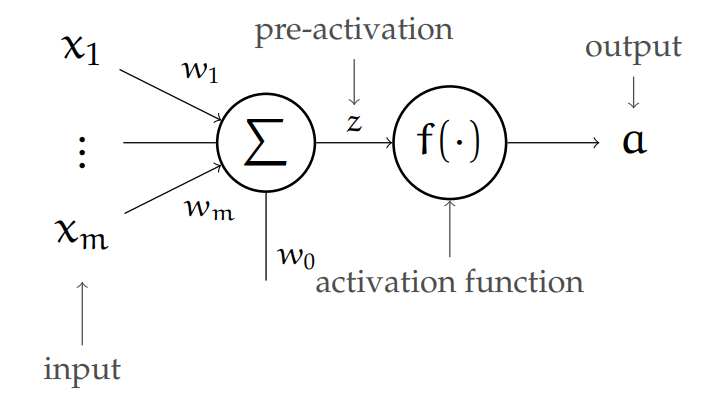
\includegraphics[scale =0.5]{Figure/ml__1.png}
    \caption{Basic structure of a neural network\cite{https://doi.org/10.48550/arxiv.1506.00619}}
    \label{fig:my_label_3}
\end{figure}




The function representing the neural network can be expressed as:

\begin{equation}\label{eq:eq1}
a= f(z) = f(\sum_{j=1}^{j=m} x_jw_j +w_0) = f(w^T x+w_0)
\end{equation}
A non-linear function of an input vector x $\in \mathbb{R}^m$ note to a single output value  a $\in$R . It is parameterized by a vector of weights  $(w_1, w_2,....w_m)\in \mathbb{R}^m$  and an offset or threshold  $w_0\in \mathbb{R}^m$ . In order for the neuron to be non-linear, we also specify an activation function  $f:\mathbb{R} \to \mathbb{R}$ , which can be the f(x)=x(linear function), or can also be any other non linear function, such as ReLU, tanh, etc., which is differentiable. 
\\
Before thinking about a whole network,let us consider how to train a single unit. \\
Given a loss function L(guess, actual) and a dataset $\{(x^{(1)},y^{(1)}),.....,(x^{(n)},y^{(n)})\}$, we can do (stochastic) gradient descent, adjusting the weights w, $w_0$ to minimize the equation \cite{LeCun2015}

\begin{equation} \label{eq:eq2}
    J(W, W_0) = \sum_{i=1} ^n L(f(x^{(i)}:W),y^{(i)})
\end{equation}
where f is the output of our neural net for a given input.

% \textbf{Provide example here :linear logistic classifiers (LLC)
% with NLL loss and regressors with quadratic loss! The activation function for the LLC is
% f(x) = $\sigma$(x) and for linear regression it is simply f(x) = x. \\
% Just for a single neuron, imagine for some reason, that we decide to use activation function f(z) = $e^z$ and loss function $L(g, a) = (g-a)^2$. Derive a gradient descent update for w and $w_0$.}

%%%%%%%%%%%%%%%%%%DO from here%%%%%%%%%%%%%%%%%%%
\subsection{Networks}


Now, we’ll try to train the network with stacking multiple neurons together to form a network. A neural network in general takes input $x \in \mathbb{R}^m$ and generates an output $\alpha \in \mathbb{R}^n $.  It is constructed with the help of multiple neurons; the inputs of each neuron might be elements of x and/or outputs of other neurons. The outputs are generated by n output units.
Here, for the training of data, we will only consider feed-forward networks. In a feed-forward network, we can think of the network as defining a function-call graph that is acyclic. For the simplicity in software and analysis, we usually organize networks into layers. A \textbf{layer} can be defined as a group of neurons which are connected to each other parallelly (as in \autoref{fig:my_label_hu}): The input of a hidden layer depends on the output of previous layer(hidden or input layer); and the output from the layers are input to the neurons in the subsequent next layer. We will start to describe about the model with a single layer and further go on to the case of multiple layers.

\subsubsection{Single-layer}
A layer is a set of unrelated entities, as  just described.  The  inputs to each unit in the layer are said to be fully connected, as shown in the figure below.  It's the same. The layer has an input x $\in\mathbb{R}^m$ and an output (also known as activation) $\alpha\in\mathbb{R}^n$
\begin{figure}[H]
    \centering
    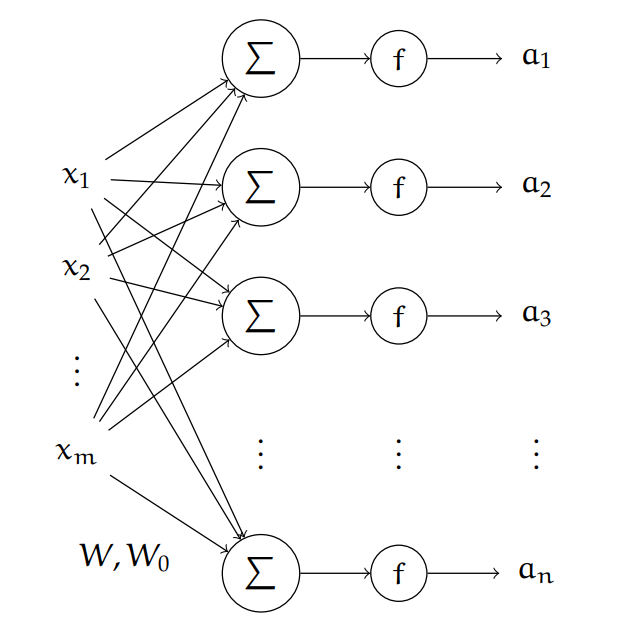
\includegraphics[scale=0.3]{Figure/ml_2.png}
    % \caption{Caption}
    \label{fig:my_label}
\end{figure}
Since each unit layer has a vector of weights and a single offset, we can consider the weights of
the whole layer as a matrix, W, and the collection of all the offsets as a vector $W_0$. If we
have m inputs, n units, and n outputs, then,
\begin{itemize}
    \item  W is an m $\times$ n matrix
     \item $W_0$ is an n$\times$  1 column vector,
     \item X, the input, is an m $\times$  1 column vector,
     \item Z = W$^T$X + $W_0$, the pre-activation, is an n$\times$  1 column vector,
\end{itemize}
and the output vector will be\\
\begin{equation*}
    A = f(Z) = f(W^Tx +W_0)
\end{equation*}

\subsubsection{Many layers}

A single neural network generally consists of multiple layers, where the output of the previous layer feeds as input to the next layer..\\
 We will use l to name a layer and 
let $m^l$ be the  number of inputs to the layer and $n^l$ be the number of outputs from the layer. Then, $W^l$ and $W^l _0$ are of shape $m^l \times n^l$, respectively. Let $f^l$ be the activation
function of layer  $ \ell$ . Then, the pre-activation outputs are the $n^l \times$ 1 vector, such that,
\begin{equation*}
    Z^l = {W^l}^T A^{l-1} + W_0^l
\end{equation*}
and the activation function outputs are simply the $n^l \times 1$ vector
\begin{equation*}
    A^l = f^l(Z^l)
\end{equation*}
We will use this structural diagram to organize our algorithmic thinking and implementation different parameters in deep neural network.
\begin{figure}[H]
    \centering
    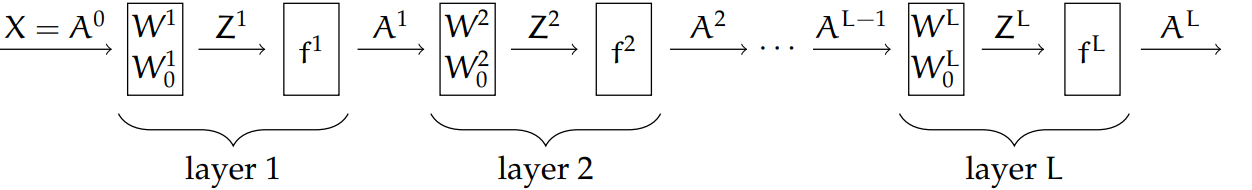
\includegraphics[scale=0.3]{Figure/ml__3.png}
    % \caption{Caption}
    \label{fig:my_label}
\end{figure}

As we saw here how a model of neural network function, the training and output from any model depends on the type of non linear functions Z, i.e. activation function we use in between the layers. Now, the question arises, how many types of activation functions are there?, and how we choose which one will be suitable for our model? We will addresses all these issues over the next section.

\subsection{ Activation function}
\label{subsection:Activationfunction}
There are three types of neural networks activation functions\cite{https://doi.org/10.48550/arxiv.1811.03378}:
\subsubsection{Binary Step Function}
Binary step function depends on a threshold value which decides whether a neuron should be activated or not. This can be represented using the equation \autoref{eq:2}

\begin{equation} \label{eq:2}
   f(x) =  \begin{cases} 
      0 for x < 0 \\
      1 for x \geq 0 
   \end{cases}
\end{equation}
The output of the equation can be represented graphically as,
\begin{figure}[H]
    \centering
    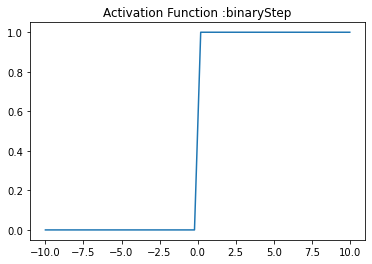
\includegraphics[scale=0.5]{Figure/binary.png}
    % \caption{Caption}
    \label{fig:my_label}
\end{figure}
The binary activation function is not always useful; a few of its limitations are:
\begin{itemize}
    \item We cannot use this activation function to provide us an output of multiclass problems, as it has only two labels of output.
    \item The gradient of the step function is zero, which causes a restriction in the back propagation process.
\end{itemize}

 
\subsubsection{Linear Activation Function}
Also known as identity Function, i.e. it can be represented using equation, and fig. below,
\begin{equation}
    f(x) = x
\end{equation}

\begin{figure}[H]
    \centering
    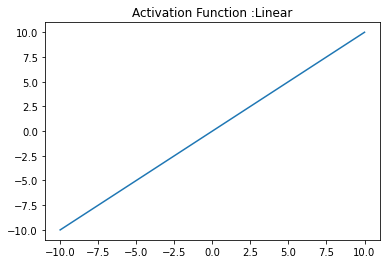
\includegraphics[scale=0.6]{Figure/linear.png}
    % \caption{Caption}
    \label{fig:my_label_02wwe}
\end{figure}

However, a linear activation function also has these two major problems :

\begin{itemize}
    \item It’s impossible to use back propagation as the gradient of the function is always a constant and has no relation with the input x.
    \item After use of linear activation function, without having dependence on a number of layers, the last layer will still be a linear function of the first layer. A linear activation function turns the neural network model into just one layer, which leads to model collapse.
\end{itemize}

 
\subsubsection{Non-Linear Activation Functions}

Non-linear activation functions solve the above limitations possessed by both linear activation functions and binary activation function as the derivative are possible and also related to the inputs, thus backpropogation are allowed here.

Few non-linear activation functions are:-\\
\textbf{Sigmoid / Logistic Activation Function}\\
Input is any real value(i.e. x $\in$ $\mathbb{R}$)and outputs $\in$ [0,1].\\
Mathematically, it can be represented as:\\
\begin{equation}
    f(x) = \frac{1}{1+e^{-x}}
\end{equation}
The output of the above equation is,
\begin{figure}[H]
    \centering
    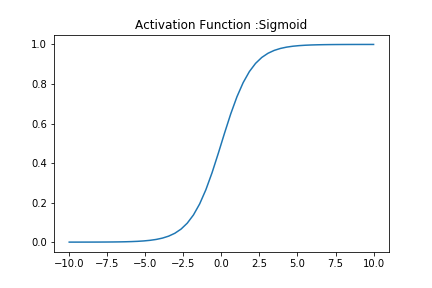
\includegraphics{Figure/sigmoid.png}
    % \caption{Caption}
    \label{fig:my_label}
\end{figure}

\textbf{Tanh Function}\\
Tanh function is very similar to the sigmoid/logistic activation function, with only difference in the output range of -1 to 1. 
Mathematically, it can be represented as;
\begin{equation}
    f(x) = \frac{e^x - e^{-x}}{e^x + e^{-x}}
\end{equation}
And, graphically, it can be represented as,\\
\begin{figure}[H]
    \centering
    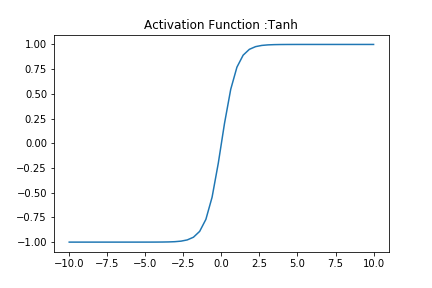
\includegraphics{Figure/Tanh.png}
    % \caption{Caption}
    \label{fig:my_label}
\end{figure}


Tanh activation function gives advantages as the output of the tanh activation function is Zero centered; thus, we can easily map the output values as strongly negative, neutral, or strongly positive. Another advantage is that the value of the hidden layers in a neural network has its values  between -1 to 1, and the mean for the hidden layer comes out to be 0 or very close to it. Therefore, it helps in centering the data and makes learning for the next layer much easier\cite{227257}.

\textbf{ReLU} \\
ReLU stands for Rectified Linear Unit. ReLU has a derivative function, despite seems like linear function. It allows backpropagation and also simultaneously making it computationally efficient. The ReLU function does not activate all the neurons at the same time. The neurons get deactivated when its output is less than 0, that is,
\begin{equation}
    f(x) = max(0,x) = \begin{cases} 
      0 & z < 0 \\
      z & otherwise 
   \end{cases}
\end{equation}

\begin{figure}[H]
    \centering
    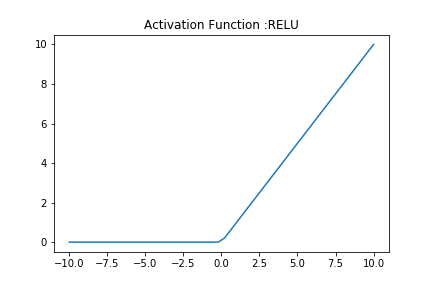
\includegraphics{Figure/RELU.png}
    % \caption{Caption}
    \label{fig:my_label}
\end{figure}


It is the most commonly used activation  function due to following unique features. Since ReLU activation function activate only a certain number of neurons, and it help them to do computation efficiently  in comparison to the sigmoid and tanh functions.\cite{https://doi.org/10.48550/arxiv.1811.03378} The ReLU activation function also increase or decrease the rate of convergence towards global minimum of the loss function due to its linear, non saturating property\cite{https://doi.org/10.48550/arxiv.1803.08375}.

\textbf{Softmax}\\
It is used to calculate the relative probabilities. Like sigmoid activation function, the SoftMax function also returns the probability of each class.
It is the most commonly used activation function for the last or output layer of the neural network in the case of multi-class classification\cite{https://doi.org/10.48550/arxiv.1811.03378}. 
Mathematically it can be represented as:
\begin{equation}
    softmax(z_i) = \frac{exp(z_i)}{\sum_j exp(z_j)}
\end{equation}
\begin{figure}[H]
    \centering
    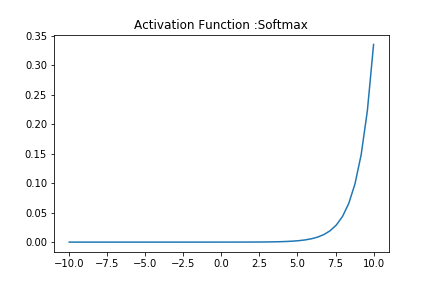
\includegraphics{Figure/softmax.png}
    % \caption{Caption}
    \label{fig:my_label}
\end{figure}
Here, we saw a few common activation functions, but how we can choose activation function for the given problem? 

\subsubsection{How to choose activation function for Hidden Layers}
The choice of activation function in between the layers depends on the type of problem we have, as it is summarized in the tree below.
 \begin{center}
    \begin{forest}
      [
      Network type?
       [Multilayer Perceptron
        [ReLU \\ Activation]
       ]
       [Convolutional Neural Net
        [ReLU \\ Activation]
         ]
        
       [Recurrent Neural Net
       [sigmoid Activation]
       [Tanh Activation]
       ]
      ] 
    %   [Multi-class\\ cross-Entropy \\Loss \\ Functions
    %   [Multi-class\\ Cross-Entropy\\ Loss]
    %   [Sparse Multiclass \\cross-Entropy \\loss]
    %   [Kullback\\ Leibler\\ Divergence \\Loss]
    %   ]
      
    \end{forest}
 \end{center}



\subsubsection{How to choose activation function for output layers}
% \begin{figure}[H]
%     \centering
%     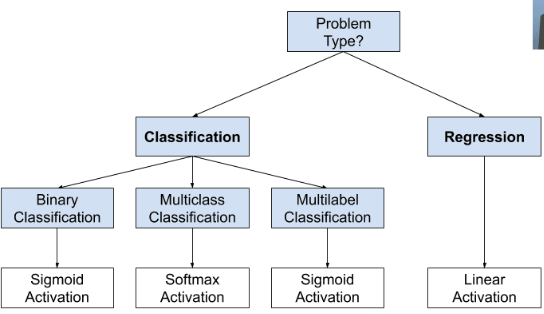
\includegraphics[scale=0.5]{Figure/ml__4.png}
%     % \caption{Caption}
%     \label{fig:my_label}
% \end{figure}
The activation function used in the last layer of the neural network depends on the type of output required and  the type of prediction problem you are trying to solve. This can be summarized from the tree below.\cite{ML_1}.
\begin{itemize}
    \item \textbf{Regression}: one node, Linear Activation
    \item \textbf{Binary Classification}:one node per class, Softmax Activation
    \item \textbf{Multiclass Classification}:One node per class, softmax activation
    \item \textbf{Multilabel Classification}: One node per class, sigmoid activation
\end{itemize}

 \begin{center}
    \begin{forest}
      [
      Problem type?
       [Classification
        [Binary \\ Classification
         [Sigmoid Activation]
        ] 
        [Multiclass \\ Classification
         [Softmax Activation]
         ]
        [Multilabel \\ Classification
        [Sigmoid Activation]
        ]
       ]
       [Regression
       [Linear Activation]
       ]
    %   [Multi-class\\ cross-Entropy \\Loss \\ Functions
    %   [Multi-class\\ Cross-Entropy\\ Loss]
    %   [Sparse Multiclass \\cross-Entropy \\loss]
    %   [Kullback\\ Leibler\\ Divergence \\Loss]
    %   ]
      ]
    \end{forest}
 \end{center}

% \begin{figure}
%     \centering
%     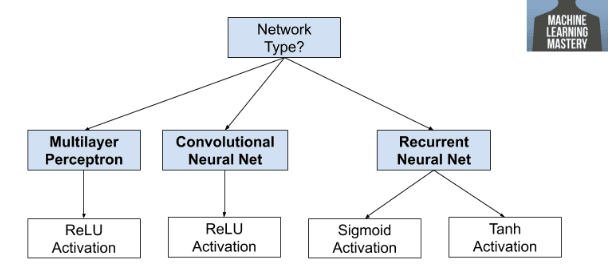
\includegraphics[scale=0.5]{Figure/ml__5.png}
%     % \caption{Caption}
%     \label{fig:my_label}
% \end{figure}















% Source
% \url{https://machinelearningmastery.com/choose-an-activation-function-for-deep-learning/}
% \url{https://www.v7labs.com/blog/neural-networks-activation-functions}
% ReLUs are especially common in internal (“hidden”) layers, and sigmoid activations are
% common for the output for binary classification and softmax for multi-class classification.(\url{https://openlearninglibrary.mit.edu/assets/courseware/v1/9c36c444e5df10eef7ce4d052e4a2ed1/asset-v1:MITx+6.036+1T2019+type@asset+block/notes_chapter_Neural_Networks.pdf}
\section{Training of Neural Network}



\subsection{Error backpropagation}
Train the neural network using the steepest descent method. You can use the batch gradient descent method, which sums the gradients of all points, or the  stochastic gradient descent method (SGD), which takes small steps with respect to the gradient after seeing one point at a time\cite{10.5555/2968826.2968922}.
% \textbf{Include theorem from} \url{https://openlearninglibrary.mit.edu/assets/courseware/v1/d81d9ec0bd142738b069ce601382fdb7/asset-v1:MITx+6.036+1T2019+type@asset+block/notes_chapter_Gradient_Descent.pdf}\\

we will always compute the gradient of the loss function with respect
to the weights for a particular value of (x, y)\cite{10.5555/2968826.2968922, https://doi.org/10.48550/arxiv.1811.03378, https://doi.org/10.48550/arxiv.1506.00619}. That tells us how much change is needed in the
weights, in order to reduce the loss experienced on this particular training. Let us understand with this example.\\
First, let’s us calculate and observe how the loss depends on the weights in the final layer, $W^L$ remembering
that our output is $A^L$, and using the shorthand loss to stand for Loss((f(x; W), y) which
is equal to Loss($A^L$, y), and finally that $A^L$ = $f^L$($Z^L$) and $Z^L$ = ${W^L}^T$ $A^{L-1}$, we can apply the chain  rule as:
\begin{figure}[H]
    \centering
    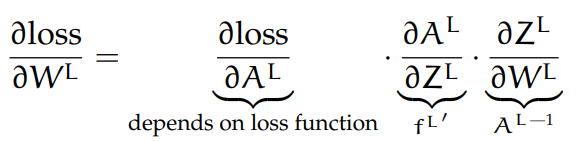
\includegraphics[scale = 0.3]{Figure/ml__6.png}
    % \caption{Caption}
    \label{fig:my_label}
\end{figure}
Here, we need to be little careful with the dimensions, and here we can note that it is true for any $ \ell$, including $ \ell$ = L\\
\begin{figure}[H]
    \centering
    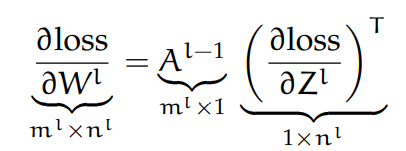
\includegraphics[scale=0.3]{Figure/ml__7.png}
    % \caption{Caption}
    % \label{fig:my_label}
\end{figure}
If  the chain rule can be applied repeatedly, we get the following equation for the loss gradient  with respect to the preactivation function of the first layer:
\begin{figure}[H]
    \centering
    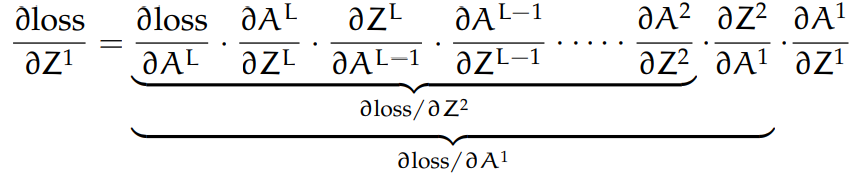
\includegraphics[scale=0.3]{Figure/ml__8.png}
    % \caption{Caption}
    \label{fig:my_label}
\end{figure}


Here,
\begin{itemize}
    \item $\frac{\partial loss}{\partial A^L}$ is $n^L \times 1$ and depends on the particular loss function you are using.
    \item $\frac{\partial Z^l}{\partial A^{l-1}}$ is $m^L \times n^L$ and is just $W^l$
    \item $\frac{\partial A^l}{\partial Z^l}$ is $n^L \times n^L$. Each element $\alpha_i ^l = f^l(z_i ^l)$. This means that $\frac{\partial \alpha_i ^l}{\partial z_j ^l}$ = 0 whenever i$\neq$ j. So, the off-diagonal elements of $\frac{\partial A^l}{\partial Z^l}$ are all 0, and the diagonal elements are $\frac{\partial \alpha_i ^l}{\partial z_j ^l}$= ${f^l}^'(z_j ^l)$
\end{itemize}
We can write the above equation as,
\begin{figure}[H]
    \centering
    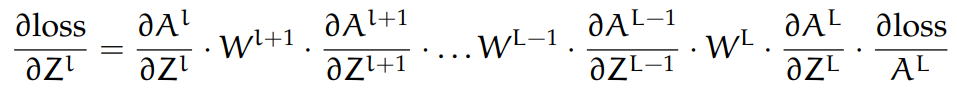
\includegraphics[scale=0.3]{Figure/ml__09.png}
    % \caption{Caption}
    \label{fig:my_label}
\end{figure}

This general process is called error back-propagation. The general idea is that we will do a forward
pass to compute all the $\alpha$ and z values at all the layers. Then, we can start work backward direction and compute the gradient of the loss with respect
to the weights in every layer, starting at last layer L and going back to layer 1, in this way model can update its weight, as can be shown below,\\
\begin{figure}[H]
    \centering
    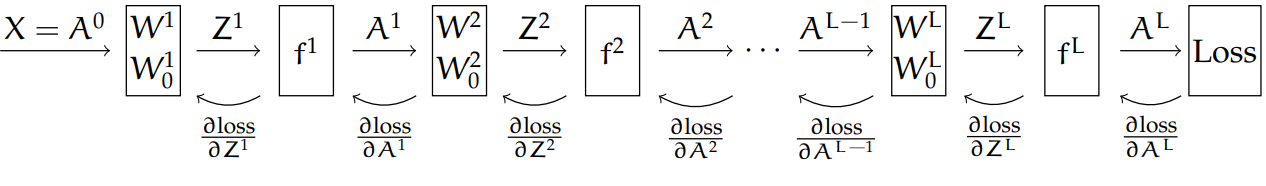
\includegraphics[scale=0.3]{Figure/ml__10.png}
    % \caption{Caption}
    \label{fig:my_label}
\end{figure}




Now, How we can do stochastic gradient descent training on a feed-forward neural network. This is the pseudo code to apply stochastic gradient descent,

% \begin{algorithm}
% \caption{\textit{SGD-NEURAL-NET(D_n,T, L, ($m^1$, ...$m^L$), ($f^1$,......,$f^L$))}}\label{alg:cap}
% \begin{algorithmic}
% \for {l=1 to L}
% \State $W_{ij} ^l ~ Gaussian(0, \frac{1}{m^l})$
% % \ $y = x^n$
% % \State $y \gets 1$
% % \State $X \gets x$
% % \State $N \gets n$
% % \While{$N \neq 0$}
% % \If{$N$ is even}
% %     \State $X \gets X \times X$
% %     \State $N \gets \frac{N}{2}$  \Comment{This is a comment}
% % \ElsIf{$N$ is odd}
% %     \State $y \gets y \times X$
% %     \State $N \gets N - 1$
% % \EndIf
% % \EndWhile
% \end{algorithmic}
% \end{algorithm}

\begin{lstlisting}[language=Python]
def SGD(f, theta0, alpha, num_iters):
    """
      Arguments:
      f -- the function to optimize, it takes a single argument
            and yield two outputs, a cost and the gradient
            with respect to the arguments
      theta0 -- the initial point to start SGD from
      num_iters -- total iterations to run SGD for
      Return:
      theta -- the parameter value after SGD finishes
    """
    start_iter = 0
    theta = theta0
    for iter in xrange(start_iter + 1, num_iters + 1):
        _, grad = f(theta)
  
        # there is NO dot product ! return theta
        theta = theta - (alpha * grad)
\end{lstlisting}



\section{Loss functions }
Now, the choice of a loss function for a particular problem is a very tedious task. We can take a rough idea about the loss function from this tree,\\
\resizebox{\linewidth}{!}{%
 \begin{center}
    \begin{forest}
      [
      Loss Function
       [Regression \\Loss\\ functions
        [Mean \\ Squared \\Error loss]
        [Mean\\ Squared \\Logarithmic \\Error loss]
        [Mean\\ absolute\\ Error\\ Loss]
       ]
       [Binary \\Classification\\ Loss \\Functions
       [Binary \\Cross- Entropy]
       [Hinge\\ Loss]
       [Squared\\ Hinge Loss]
       ]
       [Multi-class\\ cross-Entropy \\Loss \\ Functions
       [Multi-class\\ Cross-Entropy\\ Loss]
       [Sparse Multiclass \\cross-Entropy \\loss]
       [Kullback\\ Leibler\\ Divergence \\Loss]
       ]
      ]
    \end{forest}
 \end{center}
}

Like activation function, loss function also take different assumptions about the range of inputs it will take depending on the type of problem in hand. While designing the model of neural network, it become important to make things to fit well together. As, in particular, we will think about matching loss function with activation function of the last layer, $f^L$\cite{https://doi.org/10.48550/arxiv.1702.05659}. This hypothesis can be infer from the table below, \autoref{tab:my_label_12}.\\
\begin{table}[h]
    \centering
    \begin{tabular}{ccc} \hline
   \textit{   Loss }  & \textit{ $f^L$} & \textit{Comments}\\ \hline
      squared   &  Linear &  --\\
      hinge  &  Linear &  for "maximum-margin" classification\\
      NLL &   Sigmoid &   negative log likelihood loss. Useful to \\ 
      &    &       train classification problem with C classes.\\
      NLLM & softmax & -- \\
      
    \end{tabular}
    \caption{Few loss functions corresponding to the last layer/ output layer activation function. There are many different types of the loss function following the kind of problem, whether it belongs to classification or regressions. }
    \label{tab:my_label_12}
\end{table}
There are also other loss function we have used to make our model better, such as "BinaryCrossentropy", "CategoricalCrossentropy", and
"SparseCategoricalCrossentropy" belonging to probabilistic losses. Also, "mean\_squared\_error", "mean\_absolute\_error", and "MeanSquaredError" belonging to regression losses.
 
\subsubsection{Two-class classification and log likelihood}

% For classification, the natural loss function is 0-1 loss, but we have already discussed the
% fact that it’s very inconvenient for gradient-based learning because its derivative is discontinuous. \\
For binary classification problems, which are useful in separation of signal and background, Hinge loss gives us another way, to make a smoother objective, penalizing the margins of the labeled points relative to the separator. The hinge loss is defined to be
\begin{equation*}
    L_h(guess, actual) = max(1-guess.actual,0)
\end{equation*}
when actual $\in$ \{+1, -1\}
Using hinge loss with  squarednorm regularization, the learning process attempts to  find  the delimiter with the largest margin for the dataset. This optimization setting is called \textbf{Support Vector Machine}. Popular for its square shape that makes it easy to optimize SVMs\cite{https://doi.org/10.48550/arxiv.1511.08861}.

\subsubsection{Multi-class classification and log likelihood}
Multi-class classification with total of K classes, where the training label is represented with the one-hot vector $y = [y_1,...., y_k]^T$, where $y_k$= 1 if the example is of class k.Assume that our network uses softmax as the activation function (Which is most commomly used activation function for multi classification) in the last layer, so that the output is
$\alpha = [\alpha_1,....,\alpha_k]^T$, which represents a probability
distribution over the K possible classes. Then, the probability that our network predicts
the correct class for this example is $\Pi_{k=1} ^N \alpha_k ^y$ and the log of the probability that it is correct is $\sum_{k=1} ^k y_k \log \alpha_k$,so
\begin{equation*}
    L(guess, actual) = - \sum_{k=1} ^K actual_k.log(guess_k)
\end{equation*}





\section{Optimizing neural network parameters}
As neural networks consists of many parameters, our ultimate goal to minimize the loss function. The optimization can be done with help of standard gradient-descent softwares, but here, we can take advantages of the structure of the loss functions to improve optimization. The structure of loss function as a sum over terms, one training data point, help us to consider stochastic gradient methods. In this section, we will try to consider some alternative strategies for organizing training, and also to make easier to handle the step-size parameter\cite{8285338}.\\


\subsection{Batches}

Lets us assume we have an objective function of the form\\
\begin{equation*}
    J(W) = \sum_{i=1} ^n L(h(x^{(i)};W),y^{(i)})
\end{equation*}
Where h is the function calculated by the neural network and W represents all the weight matrices and vectors in the network. \\
 Use update rules when performing batch gradient descent.\\
\begin{equation*}
    W := W-\eta \nabla_W J(W), 
\end{equation*}
which is equivalent to 
\begin{equation*}
     W := W-\eta \nabla_W \sum_{i=1} ^n L(h(x^{(i)};W),y^{(i)})
\end{equation*}
Thefore, we add up the gradient of loss after each training point, with respect to W, and then take a step in the negative direction of the gradient to minimize the loss.\\


A more effective optimization strategy  is to use a mini-batch to take an "average" between the batch and the stochastic gradient descent method. For mini-batch of size k,  k different data points are evenly and randomly selected from the dataset and weight updates are performed based solely on the contribution to the gradient.
\begin{equation*}
    W \leftarrow W-\eta \nabla_W \sum_{i=1} ^n L(h(x^{(i)};W),y^{(i)})
\end{equation*}
Most neural network software packages are set up to do mini-batches\cite{25}.\\

To select k unique data points at random from a large dataset is computationally difficult. An alternative strategy, if we have an efficient procedure for randomly shuffling the data set (or randomly shuffling a list of indices into the data set) is to operate
in a loop, roughly as follows:\\
\begin{algorithm}
\caption{\textit{MINI-BATCH-SGD(NN, data, k)}}\label{alg:cap}
\begin{algorithmic}
\State $n = length(data)$
\While{not done:}
     \State $RANDOM-SHUFFLE(data)$
     \For {i=1 to $\frac{n}{k}$}
           \State $BATCH-GRADIENT-UPDATE(NN,data[(i-1)k:ik])$
% \Require $n \geq 0$
% \Ensure $y = x^n$
% \State $y \gets 1$
% \State $X \gets x$
% \State $N \gets n$
% \While{$N \neq 0$}
% \If{$N$ is even}
%     \State $X \gets X \times X$
%     \State $N \gets \frac{N}{2}$  \Comment{This is a comment}
% \ElsIf{$N$ is odd}
%     \State $y \gets y \times X$
%     \State $N \gets N - 1$
% \EndIf
% \EndWhile
\end{algorithmic}
\end{algorithm}
then, we can easily divide the dataset into k mini batches.

\subsection{ Adaptive stepsize}

Picking the value for $\eta$ is difficult and time-consuming. As our networks become deep (with increase in the numbers of layers) we can find that magnitude of the gradient of the loss with respect the weights in the last layer,$\frac{\partial loss}{\partial W_L}$,may have significant differences from the gradient of the loss with respect to the weights in the first layer $\frac{\partial loss}{\partial W_1}$.\\

The output gradient is further multiplied by all the weight matrices of the network and is “fed
back” through all the derivatives of the activation functions. This can lead to a general problem
of \textbf{exploding or vanishing gradients}, in which the back-propagated gradient is either too big
or small.

\subsubsection{Running averages}


It is a computation strategy for estimating a weighted average for a sequence of data. Let us take data sequence be $\alpha_1, \alpha_2,......;$ then we define a sequence of running average values, $A_0, A_1, A_2,....$ using the equations
\begin{equation*}
      A_0 = 0
\end{equation*}
\begin{equation*}
         A_t = \gamma_t A_{t-1} + (1-\gamma_t)\alpha_t
\end{equation*}
where $\gamma_t$ $\in$ (0,1). If $\gamma_t$ is a constant, then this is a moving average, in which
\begin{equation*}
         A_T = \gamma A_{T-1} + (1-\gamma)\alpha_T
\end{equation*}
\begin{equation*}
       = \gamma(\gamma A_{T-2} +(1-\gamma)\alpha_{T-1}) +(1-\gamma)\alpha_T
\end{equation*}
\begin{equation*}
     = \sum_{t=0} ^T \gamma^{T-t}(1-\gamma)\alpha_t
\end{equation*}
So, you can see that inputs $\alpha_t$ closer to the end of the sequence have more effect on $A_t$ than early inputs.\\


\subsubsection{Momentum}
You can use this method as well as a moving average to explain a strategy for calculating $\eta$. The easiest way is Momentum. This method "averages" the latest gradient updates and retrieves them when at least  that component of the motion vibrates in one direction. For momentum, we have\\
\begin{equation*}
      V_0 = 0
\end{equation*}
\begin{equation*}
         V_t = \gamma V_{t-1} + \eta \nabla_W J (W_{t-1})
\end{equation*}
\begin{equation*}
         W_t =  W_{t-1} - V_t
\end{equation*}
This does not look like the adaptive step size method. But if we let it do 
 If $\eta = \eta`(1 \gamma)$, the rule is similar to using the increment $\eta'$ to update to a moving average of the gradient using the parameter $\gamma$. I can see.:
\begin{equation*}
    M_0 = 0
\end{equation*}
\begin{equation*}
           M_t = \gamma M_{t-1} + (1-\gamma) \nabla_W J (W_{t-1})
\end{equation*}
\begin{equation*}
         W_t =  W_{t-1} - \eta'M_t
\end{equation*}

\begin{figure}[H]
    \centering
    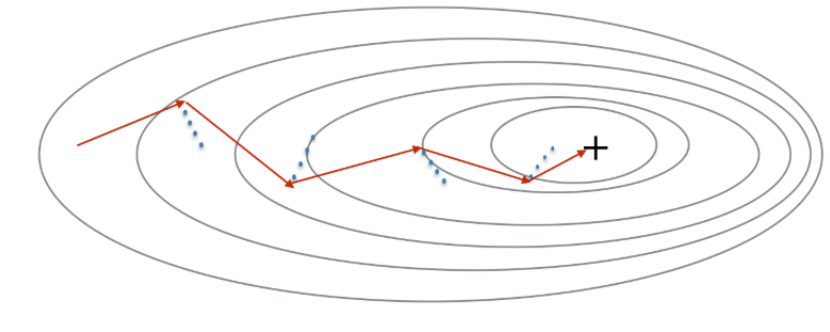
\includegraphics[scale=0.3]{Figure/ml__11.png}
    \caption{The red arrows show the change in the value of weight after one step of mini-batch gradient descent with use of momentum. The blue points show about the direction of the gradient with respect to
the mini-batch at each step. The Momentum smooths the path taken towards the local
minimum and further leads to faster convergence.\cite{21},\cite{25}}
    \label{fig:my_label}
\end{figure}

\subsubsection{Adadelta}
The idea here is to perform a large step in  the space where J(W) is almost flat (because there is no risk of the step becoming too large due to the large gradient), and if it is steep, perform a small step. That is. Apply this idea to any weight and finally get a method called Adadelta. 
 Again, the weights are indexed by the layer that contains the input and output units. Let $W_j$ be any weight in the network.\\
\begin{equation*}
    g_{t,j} = \nabla_W J (W_{t-1})_j
\end{equation*}
\begin{equation*}
       G_{t,j }= \gamma G_{t-1, j} + (1-\gamma) g_{t,j}^2
\end{equation*}
\begin{equation*}
    W_{t,j} = W_{t-1,j}- \frac{\eta}{\sqrt{G_{t,j}+\epsilon}}g_{t,j}
\end{equation*}
% The sequence $G_{t,j}$ is a moving average of the square of the jth component of the gradient.
% We square it in order to be insensitive to the sign—we want to know whether the magnitude is big or small. Then, we perform a gradient update to weight j, but divide the step
% size by $\sqrt{G_{t,j}+\epsilon}$,which is larger when the surface is steeper in direction j at point $W_{t-1}$ in weight space; this means that the step size will be smaller when it’s steep and larger when
% it’s flat.

\subsubsection{Adam}

Adam has become the most common and default method of managing step sizes neural networks. The moving averages of the gradient
and squared gradient, which estimates the mean and variance of the gradient for weight j:
\begin{equation*}
     g_{t,j} = \nabla_W J (W_{t-1})_j
\end{equation*}
\begin{equation*}
        m_{t,j} = B_1 m_{t-1,j} + (1-B_1) g_{t,j}
\end{equation*}
\begin{equation*}
        v_{t,j} = B_2 v_{t-1,j} + (1-B_2) g_{t,j}^2
\end{equation*}

If we initialize $m_0$ = $v_0$ = 0, then there will always be bias(slightly too small). So we will correct the bias by defining,
\begin{equation*}
    \hat{m}_{t,j} = \frac{m_{t,j}}{1-B_1^t}
\end{equation*}
\begin{equation*}
    \hat{v}_{t,j} = \frac{v_{t,j}}{1-B_2^t}
\end{equation*}
\begin{equation*}
    W_{t,j} = W_{t-1, j} - \frac{\eta}{\sqrt{ \hat{v}_{t,j}+\epsilon}}\hat{m}_{t,j} 
\end{equation*}
Adam did not have a huge effect on the result after making small changes in the model, which makes it an efficient method.
\section{Regularization}
So far, we've only talked about how to optimize  training data loss. As mentioned earlier, the risk of overfitting remains. This overfitting problem can be fixed by increasing the  data size. This is the case today when deep neural networks use large amounts of data. Nonetheless, there are several strategies for regularizing  neural networks, and sometimes they can be important. This can be done by implementing an early stop. This is to train in a training set and  evaluate  the current W loss in the validation set (through the entire training set or in some cases more often) at each epoch. Here, it is observed that the loss of the training set decreases fairly consistently at any number of iterations, the loss of the validation set decreases first, and then begins to increase. 
 once again. If you find that the validation loss increases systematically, you can stop training the model and return the weight with the fewest validation errors. Another easy way is to penalize  all weight criteria. This method is known as weight loss,
\begin{equation*}
    J(W) = \sum_{i=1}^n Loss(NN(x^{(i)}), y^{(i)};W) + \lambda ||W||^2
\end{equation*}
we end up with an update of the form
\begin{equation*}
    W_t = W_{t-1}(1-\lambda_\eta) - \eta (\nabla_W Loss(NN(x^{(i)}), y^{(i)};W_{t-1}))
\end{equation*}

This rule has the form of first “decaying” $W_{t-1}$ by a factor of (1 -$\lambda \eta$) and then taking a gradient step.
Other few methods are:-
% \subsection{Methods related to ridge regression}
% Early stopping is the easiest to implement and is in fairly common use. The idea is
% to train on your training set, but at every epoch (pass through the whole training set, or
% possibly more frequently), evaluate the loss of the current W on a validation set. It will
% generally be the case that the loss on the training set goes down fairly consistently with
% each iteration, the loss on the validation set will initially decrease, but then begin to increase
% again. Once you see that the validation loss is systematically increasing, you can stop
% training and return the weights that had the lowest validation error.\\
% Another common strategy is to simply penalize the norm of all the weights,This method is known as weight decay, because when we take the gradient of the objective
% \begin{equation*}
%     J(W) = \sum_{i=1}^n Loss(NN(x^{(i)}), y^{(i)};W) + \lambda ||W||^2
% \end{equation*}
% we end up with an update of the form\\
% \begin{equation*}
%     W_t = W_{t-1}(1-\lambda_\eta) - \eta (\nabla_W Loss(NN(x^{(i)}), y^{(i)};W_{t-1}))
% \end{equation*}

% This rule has the form of first “decaying” $W_{t-1}$ by a factor of (1 -$\lambda \eta$) and then taking a gradient step.


\subsection{Dropout}
The contains a simple idea, it suggest rather than perturbing the data every time we train, we will make changes in the
network. Here, we will randomly, from each dataset, after selecting a unit layer prohibit them from participating  in the training. Therefore, all  units It's a  kind of overall responsibility for  the correct answer  and can't be trusted performs all required calculations for each small subset of weights. This also tends make your network more resilient to data failures\cite{JMLR:v15:srivastava14a}.\\
When you have finished training and want to use the network to make predictions,  multiply all weights by p to get the same average activation level. Allow training forward pass\\
\begin{equation}
    \alpha^l = f(z^l) * d^l
\end{equation}
where * denotes component-wise product and $d^l$ is a vector of 0’s and 1’s drawn randomly
with probability p. The backwards pass depends on $\alpha^l$ so we do not need to make any
further changes to the algorithm.
Another modern alternative method to dropout, is batch normalization.
\subsection{Batch Normalization}

Here, idea is when training is done with mini-batches, the idea is to standardize the input values for each mini-batch, subtracting off the mean and dividing by the standard deviation of each input dimension. This gives us similar effect to adding noise and dropout. Each mini-batch of data ends up getting mildly perturbed, which prevents the network from exploiting very particular values of the data points\cite{https://doi.org/10.48550/arxiv.1502.03167}.
% So, when training with mini-batches, the idea is to standardize the input values for each mini-batch, subtracting off the mean and dividing by the standard deviation of each input dimension. This Batch normalization ends up having a regularizing effect for similar reasons that adding noise and dropout do: each mini-batch of data ends up being mildly perturbed, which prevents the network from exploiting very particular values of the data points.\\

\section{Reciever Operating Characteristic(ROC) Curve}
It is used for the performance measurement for the classififcation problems at various thresholds. ROC is a probability curve and Area-Under Curve(AUC) represents the degree or measure of separability\cite{BRADLEY19971145}. To measure the curve output after training, defined with respect to a given class \textit{C}.It tells how lots version is able to distinguishing among classes. Given a point x and model that outputs a P(C|x) probability that x belongs to the class C. Given T , a threshold, x belongs to C if and only if P(C|x) $\geq$ T . If T = 1, a point is labeled as belonging to class, C only if the model is 100\% sure. If T = 0, every point is labeled as belonging to the class C\\
The ROC curve is the curve generated by traveling from T = 0 to T = 1 with each value of the threshold T generating a point (False Positive, True Positive)\cite{Melo2013, Hajian-Tilaki2013}. The different ROC curves based on output may be observed in \autoref{fig:my label-2}. A good model will have a curve that climbs quickly from 0 to 1.. 
\begin{figure}[H]
    \centering
    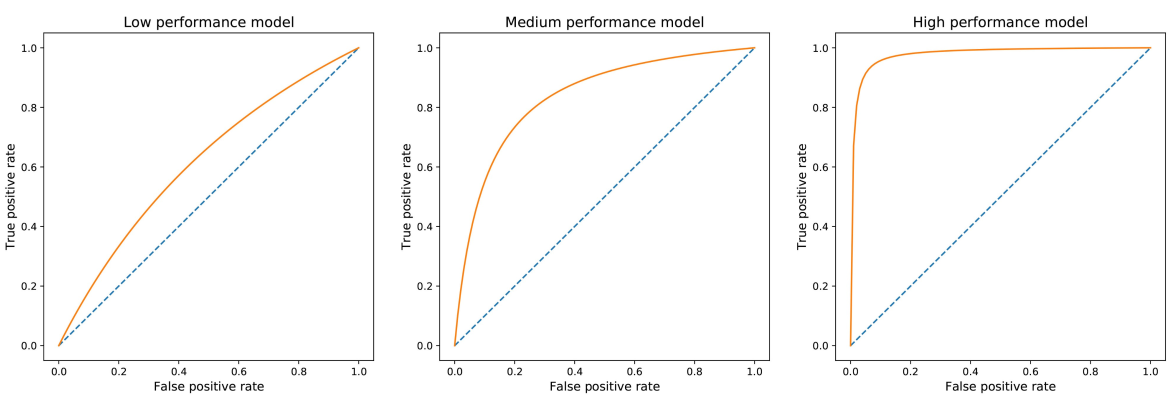
\includegraphics[scale=0.3]{Figure/13__ml.png}
    \caption{ROC curves depending on the effectiveness of the model}
    \label{fig:my_label-2}
\end{figure}

Few defining terms:-\\
\textbf{TPR (True Positive Rate) / Recall /Sensitivity)} \\

\begin{equation*}
    TPR (True Positive Rate) / Recall /Sensitivity) = \frac{TP}{TP+FN}
\end{equation*}

\textbf{Specificity}\\
\begin{equation*}
    Specificity = \frac{TN}{TN+FP}

\end{equation*}

\textbf{FPR} \\
\begin{equation*}
    FPR = 1- Specificity
        = \frac{FP}{TN+FP}
\end{equation*}







%     \textbf{(Maths part may be excluded)}



% 1. \url{https://openlearninglibrary.mit.edu/assets/courseware/v1/9c36c444e5df10eef7ce4d052e4a2ed1/asset-v1:MITx+6.036+1T2019+type@asset+block/notes_chapter_Neural_Networks.pdf}

% \url{https://www.mygreatlearning.com/blog/types-of-neural-networks/}
% \url{MIT lecturre from where you have learnt}



\setcounter{equation}{0}
\setcounter{table}{0}
\setcounter{figure}{0}
%\baselineskip 24pt

\clearpage
\chapter{\label{signal_background}Signal and Background}
% \begin{itemize}
%     \item Write about the how the smaples are generated 
%     \item How you applied the cuts 
%     \item how the DNN are [erforming for the background and signal separation?
%     \item discuss about the vaialbes.    
% \end{itemize}


Monte Carlo simulations are used to model pp collisions at the LHC. Various processes are generated based on their cross-sections, kinematics and the dynamics of the interaction. MC samples for both signal and background events were produced by the CMS generator team. 
The signal process, pp $\longrightarrow$ $T{’}$bq, is generated at leading order using the Monte Carlo (MC) event generator MADGRAPH5\_AC@NLO 2.3.3 \cite{Alwall2014, Artoisenet2013}for various masses of $T{’}$ quark and for the decay $T'\longrightarrow tH$. The decay of Higgs boson(H$\longrightarrow \gamma \gamma$) is simulated using PYTHIA 8.2 \cite{SJOSTRAND2015159}. The $T{’}$ quark masses used for final results range from 600 to 1200 GeV. The mass of the Higgs boson is set to 125 GeV and the mass of the top quark is set to 172.5 GeV. The NNPDF3.0 parton distribution function is used \cite{Ball_2015} . The signal samples are generated for left-handed chirality of $T{’}$ quark. The simulated signal samples with their cross section can be seen in the \autoref{tab:my_labeL_Signal} \\
As for background MC samples, various generators are exploited: MADGRAPH5\_AMC@NLO 2.2.2 (MG5\_AMC), PYTHIA 8.2\cite{SJOSTRAND2015159}, SHERPA 2.2 \cite{10.21468/SciPostPhys.7.3.034}. For the 2016 MC production, the PYTHIA tune CUETP8M1 \cite{Khachatryan2016} is used, while for the 2017 and 2018 MC productions, the PYTHIA tune CP5 \cite{Sirunyan2020} is adopted. \\
Two types of SM background are considered in the analysis according to their shapes in the di-photon invariant mass spectrum: resonant background (SMH) and non-resonant background (NRB). The former refers to the SM Higgs production processes while the latter refers to other SM processes that have non-negligible contributions to the analysis. The simulated background samples with their cross section can be seen in the \autoref{tab:my_label_BAckground}\\
The major SM Higgs production modes are produced with MG5 a MC@NLO interfaced with PYTHIA 8.2, including gluon fusion \cite{Bagnaschi_2012}, vector boson fusion, production in association with with top quarks \cite{PhysRevD.91.094003}, and with a vector boson. The total cross-sections and branching ratios recommended by the LHC cross-section working group  are used.

For the non-resonant background, di-photon samples, in which two prompt photons not forming a peak, are simulated by SHERPA 2.2. QCD multi-jets events (contributing two fake photons) and gamma + jets processes (offering one prompt photon and one fake photons) are simulated by PYTHIA 8.2, with a ”Double EM-enriched” filter applied during production. 


After generation, events are propagated through the simulation of the CMS detector using the
Geant4\cite{AGOSTINELLI2003250} package. The effects of multiple proton-proton interactions are also modeled in the package by adding simulated minimum-bias interactions to the simulated samples. The number of pileup interactions agrees with the one observed in data after reweighting the simulated pileup distribution, with the recommended 69.2 mb minimum bias cross-section.


\begin{table}[H]
    \centering
    \resizebox{\textwidth}{!}{
    \begin{tabular}{|c|c|c|} \hline
     Sample Name    & $T^'$ Mass  & Cross-Section(fb) \\
                    & (${GeV}/{c^2}$) & 13TeV\\ \hline
 TprimeBToTH\_Hgg\_M-600\_LH\_TuneCP5\_PSweights\_13TeV-madgraph\_pythia8.root    &  600 & 1.161 \\
 TprimeBToTH\_Hgg\_M-625\_LH\_TuneCP5\_PSweights\_13TeV-madgraph\_pythia8.root    & 625 & 0.939 \\
 TprimeBToTH\_Hgg\_M-650\_LH\_TuneCP5\_PSweights\_13TeV-madgraph\_pythia8.root    & 650 & 0.717 \\
 TprimeBToTH\_Hgg\_M-675\_LH\_TuneCP5\_PSweights\_13TeV-madgraph\_pythia8.root  & 675 & 0.586  \\
 TprimeBToTH\_Hgg\_M-700\_LH\_TuneCP5\_PSweights\_13TeV-madgraph\_pythia8.root    & 700  & 0.455 \\\hline \hline
 TprimeBToTH\_Hgg\_M-800\_LH\_TuneCP5\_PSweights\_13TeV-madgraph\_pythia8.root    & 800 & 0.196\\
  TprimeBToTH\_Hgg\_M-900\_LH\_TuneCP5\_PSweights\_13TeV-madgraph\_pythia8.root   & 900  & 0.0903 \\
  TprimeBToTH\_Hgg\_M-1000\_LH\_TuneCP5\_PSweights\_13TeV-madgraph\_pythia8.root   & 1000  &  0.0440\\ \hline \hline
  TprimeBToTH\_Hgg\_M-1100\_LH\_TuneCP5\_PSweights\_13TeV-madgraph\_pythia8.root  & 1100  &   0.0224 \\
  TprimeBToTH\_Hgg\_M-1200\_LH\_TuneCP5\_PSweights\_13TeV-madgraph\_pythia8.root   &  1200  & 0.0118	\\ \hline
    \end{tabular}}
    \caption{List of Monte Carlo signal samples used in the analysis with their cross-section\cite{CrossSection_1}.} 
    \label{tab:my_labeL_Signal}
\end{table}



\begin{table}[H]
    \centering
    \resizebox{\textwidth}{!}{
    \begin{tabular}{|c|c|c|} \hline
    Standard Model Higgs background    & Cross-Section \\
                   & $\times$ BR(H$\longrightarrow \gamma \gamma$)(fb)\\ \hline
  ttHJetToGG\_M125\_13TeV\_amcatnloFXFX\_madspin\_pythia8.root   &  1.15 \\
   THQ\_ctcvcp\_HToGG\_M125\_13TeV-madgraph-pythia8.root & 0.17 \\   
 GluGluHToGG\_M125\_TuneCP5\_13TeV-amcatnloFXFX-pythia8.root & 110.28 \\  
 VBFHToGG\_M125\_13TeV\_amcatnlo\_pythia8.root  &  8.59 \\
VHToGG\_M125\_13TeV\_amcatnloFXFX\_madspin\_pythia8.root & 5.12\\\hline \hline
   Non-resonant background      &    Cross-Section (pb)  \\ \hline
   output\_TTJets\_pythia8.root   &     722.8 \\ 
   output\_TTGG\_0Jets\_pythia8.root  &  0.01687\\
   output\_TGJets\_pythia8.root  &  2.967  \\
   output\_GJet\_Pt-40toInf\_DoubleEMEnriched\_MGG-80toInf\_pythia8.root & 878.1\\
   output\_DiPhotonJetsBox\_MGG-80toInf\_13TeV-Sherpa.root    &   84.4  \\\hline
    \end{tabular}}
    \caption{List of background samples. \cite{crossSection_2, crossSection_3}}
    \label{tab:my_label_BAckground}
\end{table}

\section{Variable Selections}
\subsection{Primary Vertex Selection}
Events to analyze should satisfy the following conditions:
\begin{itemize}
    \item At least one good primary vertex with n.d.o.f. $\geq$4.
    \item The track impact parameter with respect to the beam spot on the z axis, |z| , should be within 24 cm
    \item The track impact parameter with respect to the beam spot on the x-y plane, |$\rho$|, should be smaller than 2 cm
\end{itemize}

\subsection{Photons}
Photons are reconstructed with the energy deposits of the electromagnetic calorimeter (ECAL). Not associated with the tracker's charged particle track due to incomplete simulation, detection effect and energy loss correction by converted photons in  tracker by considering the following physical quantities:
\begin{itemize}
    \item Shower shape and isolation variables
    \item Energy scales and smearing
\end{itemize}


Photon identification MVA is an important algorithm used to isolate ("prompt") photons and false photons in a jet from quark / gluon fragmentation and hadronization. Training is  based on DNN(Deep Neural Network) and BDT(Boosted Decision Trees) using simulated samples. 
 Analysis of $\gamma$+ jets events using prompt photons  as signals while using fake photons from jets as a background. The training takes the corrected shower shape and isolation variables as the input features. 
 
 
 In the analysis, any two photons in an events forms a di-photon candidates. For each di-photon candidate, $p_T$ cuts  are imposed for the leading (sub-leading) photon to maintain a smooth shape of the $m_{\gamma\gamma}$ distribution. Since $\frac{p_T}{m_{\gamma\gamma}}$ has a dependency on the opening angle between two photons, imposing the $\frac{p_T}{m_{\gamma\gamma}}$ can prevent a bad resolution of diphoton invariant mass as well \autoref{eq:equation_6}. This selection is standard in the H$\longrightarrow \gamma\gamma$ analysis.
 
 \begin{equation}\label{eq:equation_6}
     m_{\gamma_1\gamma_2} = \sqrt{E_{\gamma_1}E_{\gamma_2}(1- \cos{\theta_{\gamma_1\gamma_2}})}
 \end{equation}
 
 For each photon, photon ID MVA score is required to be larger than −0.7, which eliminates
reducible background events without loosing much VLQ signal events in the H$\longrightarrow \gamma\gamma$ channel.
If there are more than one di-photon candidate surviving all the event selections in an event, the candidate with the largest scalar sum of two photons $p_T$ is chosen as the Higgs candidate of the event.

Invariant mass of the leading two photons is further used to define the signal window and the sideband regions:
\begin{itemize}
    \item Signal window: $m_{\gamma\gamma} \in$ [115, 135]GeV
    \item Sideband region: $m_{\gamma\gamma} \in$ [110, 115] $\cup$ [135, 180]GeV.
\end{itemize}
The signal window is blinded throughout the development of the analysis.

\subsection{Jets}

We follow the standard recommendations from JetMET physics object group for treatments of jets. Reconstruction of jets is based on anti-kT clustering algorithm \cite{Cacciari_2008} with a distance parameter being 0.4 (AK4). The jets originate from particle flow candidates with charged hadron coming from non-primary vertices subtracted (PFchs). The jet energy corrections and energy smearing are applied according to the recipes provided by the JERC group\cite{CrossSection_5}.

\subsection{b-tagged jets}
Jets originating from the hadronization of b-quarks are tagged using the DeepCSV algorithm. The loose working point of the DeepCSV algorithm is used to identify b jets. Additionally, the b jets are required to be in the barrel region ( |$\eta$| < 2.5). 


\subsection{Missing ET}
The missing transverse momentum vector $\Bar{P_T}^ {miss}$ is computed as the negative vector sum of the transverse momenta of all the PF candidates in an event. The magnitude of $\Bar{P_T}^ {miss}$ is denoted as MET. In the analysis, MET considers the standard type 1 correction (JEC propagation) while the variation of MET uncertainty considers effects from JEC and unclustered energy.

The different variable used in this analysis are listed in \autoref{tab:my_label_Variable}

  \begin{table}[h!]
    \centering
    \resizebox{6cm}{!}{
    \begin{tabular}{|c|c|}\hline
     Sl. No.    & Variables \\\hline
       1  & dipho\_leadPt \\
        2  & dipho\_mass\\
         3  & dipho\_leadEta \\
          4  & dipho\_leadIDMVA \\
           5  & dipho\_subleadIDMVA \\
            6  & dipho\_lead\_haspixelseed \\
             7  & dipho\_sublead\_haspixelseed \\
              8  & n\_jets \\
               9  & n\_bjets \\
                10  & n\_centraljets \\
                 11  & lepton\_charge \\
                  12  & lepton\_leadPt \\
                   13  & lepton\_leadEta \\
                    14  & fwdjet1\_pt \\
                     15  & fwdjet1\_eta \\
                      16  & fwdjet1\_discr \\
                       17  & top\_mt\\
                        18  & dr\_tHchainfwdjet \\
                         19  & dr\_leptonbjet \\
                          20  & dr\_leptonfwdjet\\
                          21  & dr\_bjetfwdjet \\
                            22  & dr\_leadphofwdjet\\
                             23  & dr\_subleadphofwdjet \\
                              24  & bjet1\_pt\\
                              25 & bjet2\_pt \\
                              26  & bjet3\_pt \\
                               27 & bjet1\_eta \\
                              28  & bjet2\_eta \\
                                29  & bjet3\_eta \\
                                  30  & bjet1\_discr\\
                                    31  & bjet2\_discr \\ 
                                    32 & bjet3\_discr \\
                                   33  &   jet1\_pt \\
                                    34  &  jet2\_pt  \\
                                   35    &  jet3\_pt  \\
                                  36      &  jet1\_eta  \\
                                 37        & jet2\_eta   \\
                                 38         &  jet3\_eta  \\
                                    39       &  jet1\_discr  \\
                                      40      &  jet2\_discr  \\
                                       41      &   jet3\_discr \\
                                       42       &  dipho\_subleadEta  \\
                                    
                                    
                                    
                                    \hline
           
    \end{tabular}}
    \caption{Variables of signal and Background used as input variable of the DNN model and further used as testing}
    \label{tab:my_label_Variable}
\end{table}





Even when intriguing particles are created, finding them is a difficult task. They have very small cross-section compared to the other particles. Although new particles cannot be seen directly, the lighter stable particles to which they decay, known as decay products, can be seen in the detector. For this reason, multiple layers of detectors surround the moment of impact. Each decay product interacts with these detectors in a way that permits the direction and momentum of the decay product to be detected. The signal $T{'}$ have the final product of bottom quark(q), leptons(electon and electron neutrino), and diphoton($\gamma\gamma$). The backgrounds Standard Model Higgs(SMH) and Non-Resonant background (NRB) have similar final state topology.

Electrically charged leptons (electrons or muons, designated) and particle jets are visible decay products (collimated streams of particles originating from quarks or gluons, denoted j).The synthesis of top quarks in pairs ($\Bar{t}tH$)  or singly (tH) with the Higgs boson allows direct experimental access to the top-Higgs interaction with an output signature comparable to that of  $\Bar{t}tH (tH)$ decay. The ttH (tH) production mode has a highly distinctive experimental signature, which includes leptons and/or jets from the decay of the two (single) top quarks, as seen in \autoref{fig:my_label_tth}, while proceeding at a rate roughly 100(1000) times slower than gluon fusion.\\
The ttH production cross section is predicted to grow by a factor of four as the LHC energy is increased from 8 to 13 TeV for Run 2. However, such a mechanism is still uncommon, and searches for ttH creation have been fueled by the increased sensitivity achieved in Higgs decay modes with higher branching fractions. \\
\begin{figure}[H]
    \centering
    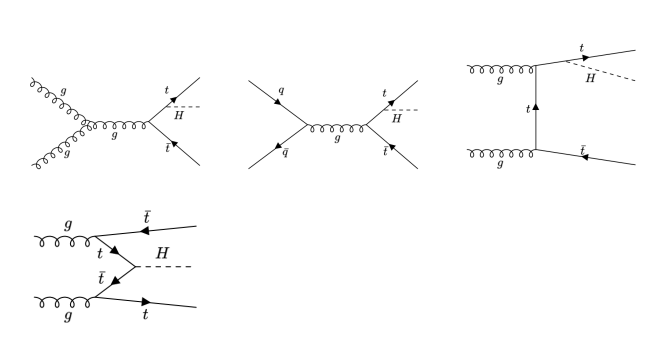
\includegraphics[scale=0.7]{figure_1/tth_1.png}
    \caption{Feynman diagrams depicting $t\Bar{t}H$ production modes}
    \label{fig:my_label_tth}
\end{figure}
The T$^'$ quark could couple to bW, tZ, or tH, resulting in the corresponding T$'$ quark decays as shown with Feynman diagram in the \autoref{fig:my_label_T'}. All the other few backgrounds with similar decay signature used as the backgrounds are shown in \autoref{fig:my_label_ttgg}, \autoref{fig:my_label_thq}, and \autoref{fig:my_label_ttgg_12}.\\


\begin{figure}[H]
    \centering
    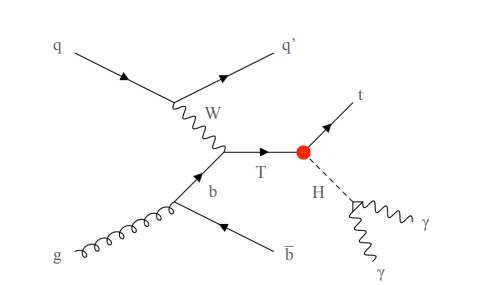
\includegraphics[scale=0.5]{figure_1/T'.png}
    \caption{Leading-order Feynman diagram for single T’ production}
    \label{fig:my_label_T'}
\end{figure}


\begin{figure}[H]
    \centering
    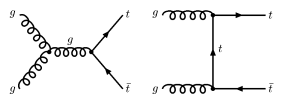
\includegraphics[scale=0.7]{figure_1/ttgg.png}
    \caption{ttgg Feynman diagram}
    \label{fig:my_label_ttgg}
\end{figure}

\begin{figure}[H]
    \centering
    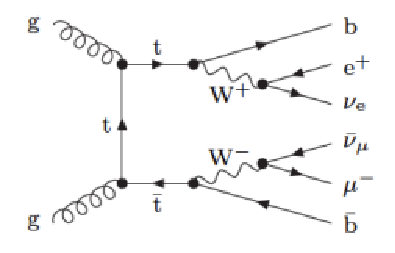
\includegraphics[scale=1]{figure_1/ttgg__.pdf}
    \caption{Feynman diagram for ttgg}
    \label{fig:my_label_ttgg_12}
\end{figure}


\begin{figure}[H]
    \centering
    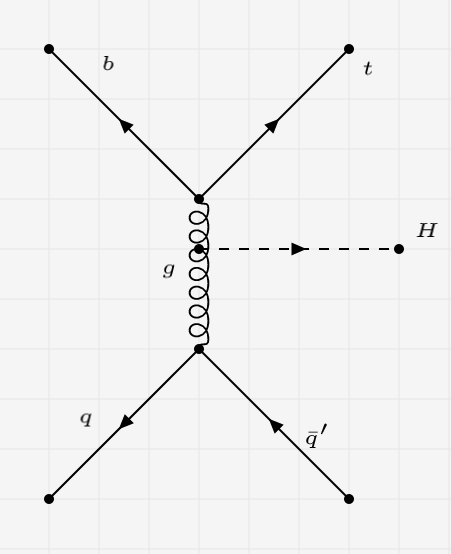
\includegraphics[scale =1]{figure_1/thq.png}
    \caption{Feynman diagram of thq}
    \label{fig:my_label_thq}
\end{figure}




Few of the plots of variables of these simulated samples are shown in  \autoref{fig:Signal_bkg_plotting} showing the high level input features on the right side of \autoref{fig:Signal_bkg_plotting} and low level input features on the left of \autoref{fig:Signal_bkg_plotting}.
\begin{figure}[H]
\begin{subfigure}{.5\textwidth}
  \centering
  % include first image
  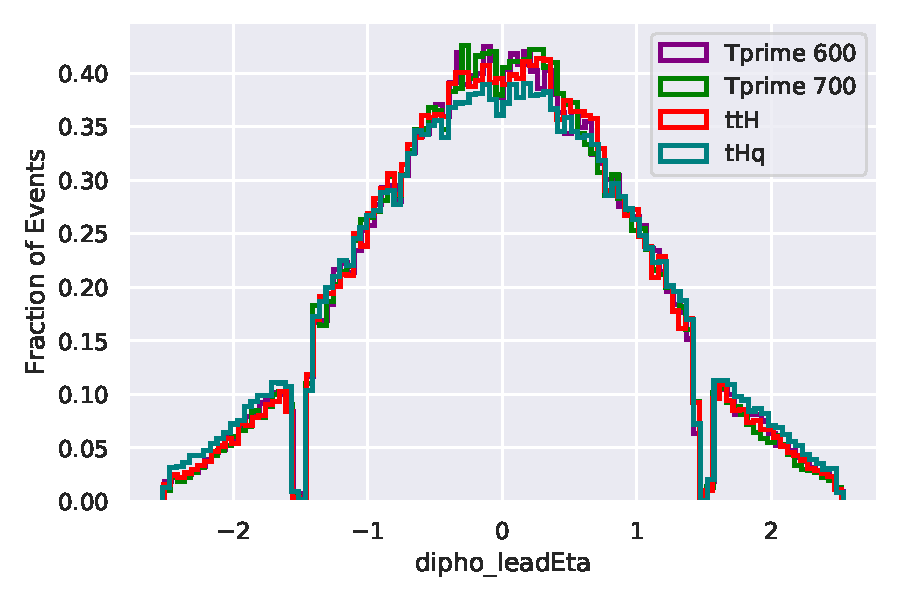
\includegraphics[width=.8\linewidth]{Figure_2/dipho_leadEta.pdf}  
  \caption{}
  \label{fig:sub-first}
\end{subfigure}
\begin{subfigure}{.5\textwidth}
  \centering
  % include second image
  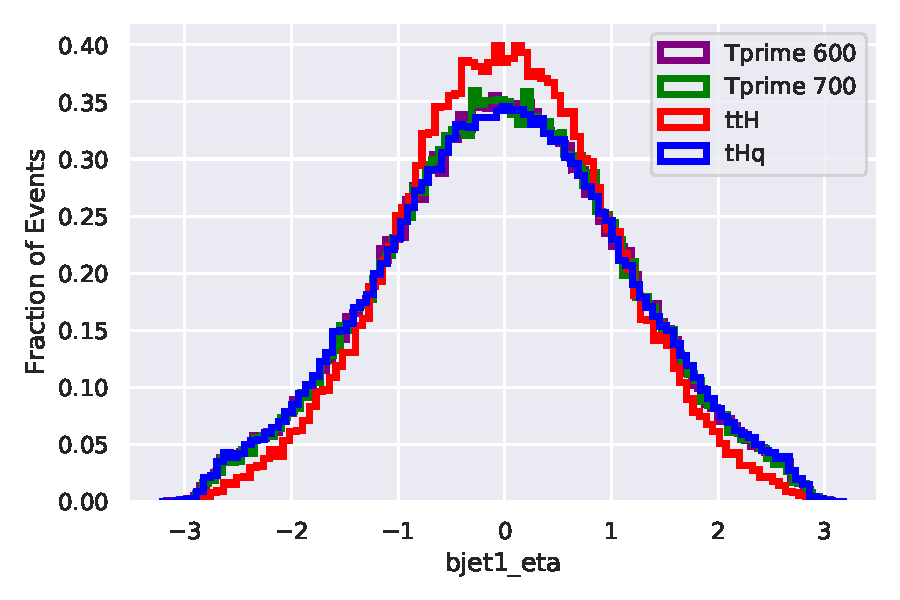
\includegraphics[width=.8\linewidth]{Figure_2/bjet1_eta.pdf}  
  \caption{}
  \label{fig:sub-second}
\end{subfigure}



\begin{subfigure}{.5\textwidth}
  \centering
  % include third image
  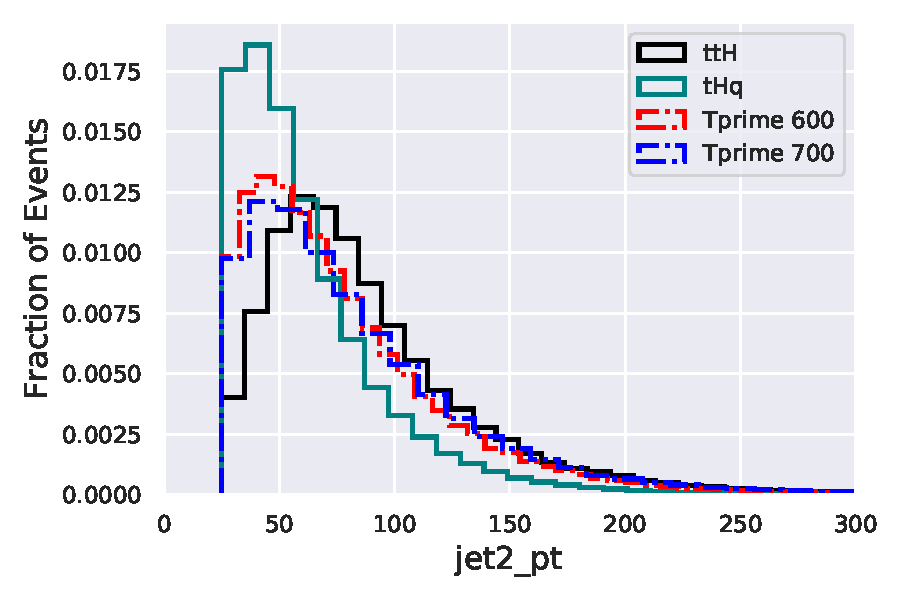
\includegraphics[width=.8\linewidth]{Figure_2/jet2_pt.pdf}  
  \caption{}
  \label{fig:sub-third}
\end{subfigure}
\begin{subfigure}{.5\textwidth}
  \centering
  % include fourth image
  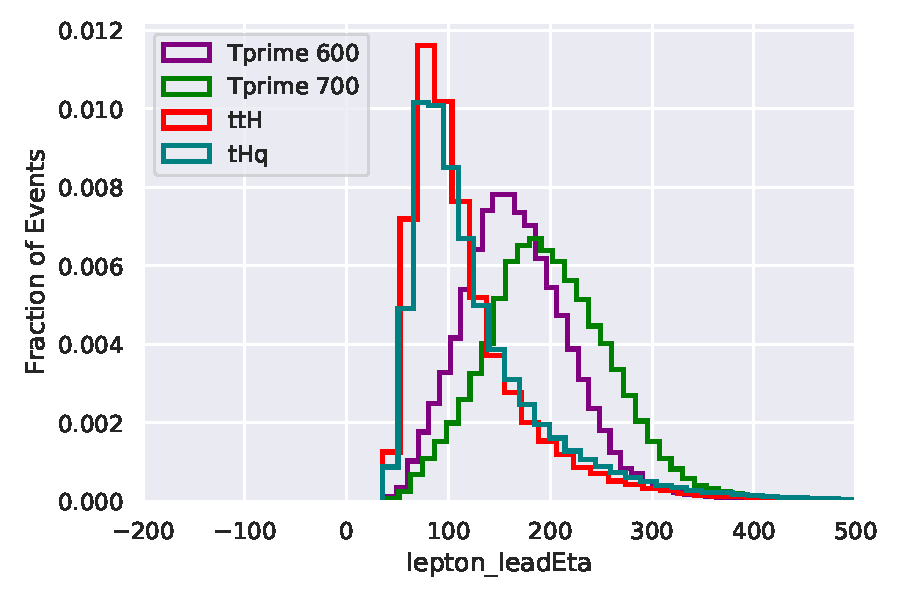
\includegraphics[width=.8\linewidth]{Figure_2/dipho_leadPt.pdf}  
%   \caption{}
  \label{fig:sub-fourth}
\end{subfigure}


\begin{subfigure}{.5\textwidth}
  \centering
  % include third image
  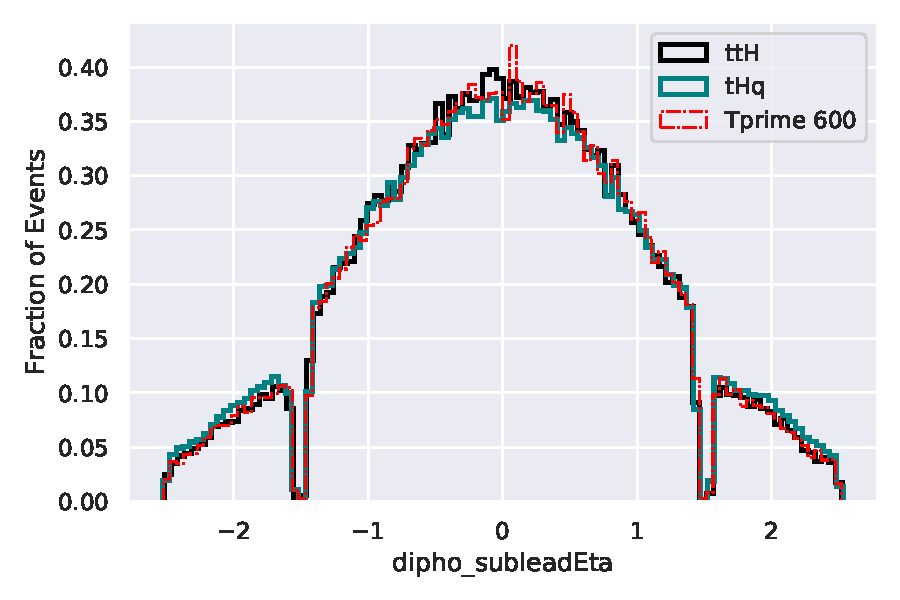
\includegraphics[width=.8\linewidth]{Figure_2/dipho_subleadEta.pdf}  
%   \caption{}
  \label{fig:sub-fifth}
\end{subfigure}
\begin{subfigure}{.5\textwidth}
  \centering
  % include fourth image
  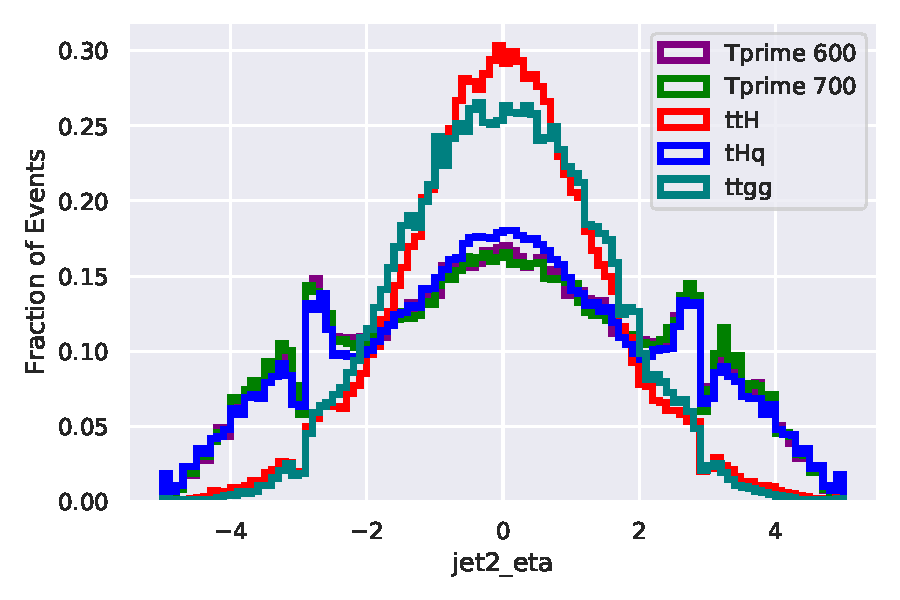
\includegraphics[width=.8\linewidth]{Figure_2/jet2_eta.pdf}  
%   \caption{}
  \label{fig:sub-fourth}
\end{subfigure}

\begin{subfigure}{.5\textwidth}
  \centering
  % include third image
  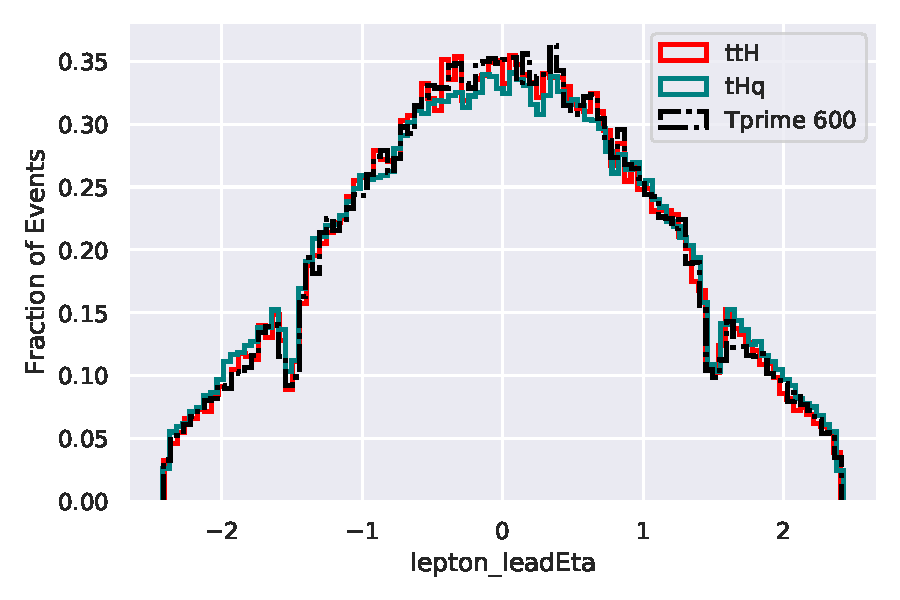
\includegraphics[width=.8\linewidth]{Figure_2/lepton_leadEta.pdf}  
%   \caption{}
  \label{fig:sub-third}
\end{subfigure}
\begin{subfigure}{.5\textwidth}
  \centering
  % include fourth image
  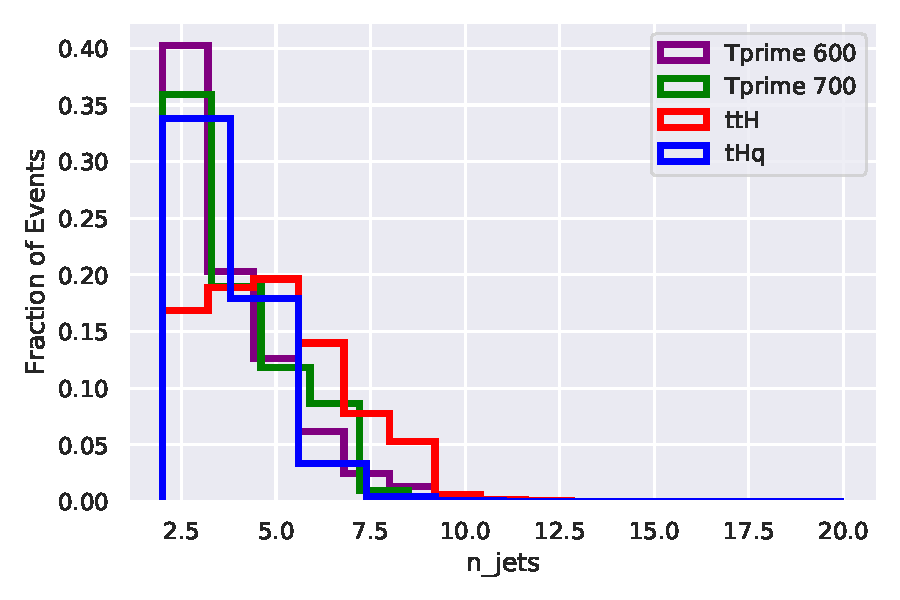
\includegraphics[width=.8\linewidth]{Figure_2/n_jets.pdf}  
%   \caption{}
  \label{fig:sub-fourth}
\end{subfigure}
\caption{Simulated sample plot for different variables, for each figure plotted above the signal is Tprime and the standard model higgs as the background. From top to bottom, plots for different variable are as, (a) Plot for dipho\_leadEta, (b) Plot for bjet1\_eta, (c)Plot for jet2\_Pt, (d) Plot for dipho\_leadPt, (e) Plot for dipho\_subleadEta, (f) Plot for jet2\_eta, (g) Plot for lepton\_leadEta, and (h) Plot for n\_jets  }
\label{fig:Signal_bkg_plotting}
\end{figure}
 
In the given \autoref{fig:Signal_bkg_plotting}, even from the best separation among the input variable of the Tprime(signal) and SMH(background) model of the monte carlo smaples, we cannot see how our signal (Tprime) get clearly separated from the standard model higgs(SMH) backgrounds. 
For the better separation between these two, we need the application of machine learning techniques(DNN), which discussed in details with outputs in \autoref{AN}, \autoref{R_D}.
For the testing for the presence of any signals in the \textit{RUN II} datafile,  the DNN training model have been tested on \textit{"allData\_RunII.root"}, which collected by CMS data acquisition team during 2016, 2017, 2018 run of the LHC, with an integrated
luminosity of 137.65$fb^{-1}$ , is used for this analysis.




% \noindent\fbox{%
%     \parbox{\textwidth}{%
%         1. In the signal hypothesis we expect that: 
%         2. Write what expect in the background hypothesis.
%         3. 
%     }%
% }








\setcounter{equation}{0}
\setcounter{table}{0}
\setcounter{figure}{0}
%\baselineskip 24pt


% %%%%%%%%%%%%%%%%%%%%%%QUESTIONS MAY GET FRAMED FROM HERE%%%%%%%%%%%%%%%%%%%%%%%%%%%%%%%%%%%%%%%%%%%%%%
% \begin{itemize}
%     \item Why we measure luminosity in $fb^{-1}$
% \end{itemize}
\clearpage
\chapter{\label{AN}Analysis Strategy}
% \begin{itemize}
%     \item Address all the basic questions.
%     \item write about all the simulations.
%     \item Add table on hoe you have applied cut
% \end{itemize}




The analysis done for the events where one vector-like quark, $T’$, is produced and then decays into a top quark and a Higgs boson decaying into two photons. Further, we wish to set upper limits on the cross-section of the vector-like quark $T’$ with $M_{T’}$ in the range of [600, 1200] GeV.

The Higgs invariant mass (or diphoton invariant mass, $m_{\gamma\gamma}$ ) is the main probe of the analysis. The photons and di-photon Higgs candidates are reconstructed using the flashgg framework\cite{CrossSection_6}.
 Two mass regions are defined accordingly:
\begin{itemize}
    \item Signal window:  $m_{\gamma\gamma}$ $\in$ [115, 135]GeV
    \item Sideband region: $m_{\gamma\gamma}$ $\in$ [100, 115]$\cup$[135, 180]GeV
\end{itemize}
where the signal window is blinded throughout the development of the analysis.



Misclassification is less likely when optimal discrimination is used. In this regard, the typical method of selecting and applying cuts to one event variable at a time is rarely optimal. If correlations exist between a collection of event variables (denoted by a vector x), optimal separation may always be achieved if the variables are treated in a fully multivariate fashion. The best technique to partition a multidimensional space occupied by two classes of events, such as's' and 'b,' is to use a cut on the probability ratio,

\begin{equation}
    r(\textbf{x}) = \frac{p(s|\textbf{x})}{p(b|\textbf{x})} = \frac{p(\textbf{x}|s) p(s) }{p(\textbf{x}|b) p(b) }
\end{equation}

where  p(\textbf{x}|s) and p(\textbf{x}|b) are the class conditional probabilities, i.e., probability density functions for signal and background, and p(s) and p(b) are the prior probabilities.
 As a result, the posterior probability for the desired class's' is
 
\begin{equation}
    p(s|\textbf{x}) = \frac{r}{1+r} = \frac{ p(s|\textbf{x}) p(s)}{p(\textbf{x}|s)p(s) +  p(\textbf{x}|b)p(b)}
\end{equation}

The Bayes discriminant is the discriminant 'r'. Calculating the Bayes discriminant r(x) or the class conditional probabilities lowers the discrimination problem quantitatively. It's worth noting that, curiously, techniques like neural networks may directly produce the posterior probability p(s|\textbf{x}).



Here preselections are defined to maintain high efficiency in the signal events. To targets the leptonic decays of the top quark. These were done:-
\begin{enumerate}
    \item The binary classification algorithms (Deep Neural Network, DNN) with simulated samples of VLQ as signal and simulation of the related Standard Model processes as background with the following specifications, with one DNN is trained: only the Standard Model Higgs production modes are included as background during training.

\item Define a signal region by rectangular cuts on DNN scores. The cuts are determined such that the significance is maximized.

\item Construct parametric signal and background models from the fits to$m_{\gamma\gamma}$ distribution in each defined signal region. 
\item Non-resonant background are modeled from data in $m_{\gamma\gamma}$  sideband with a variety of functional from. The choice of functional from is treated as a discrete nuisance parameter, following the discrete profiling method. In particular, the fit is performed per year and per channel to capture the year-dependent $m_{\gamma\gamma}$ resolution. In the end, we perform a simultaneous fit of the $m_{\gamma\gamma}$  spectra in the signal regions only for the leptonic channel to extract a limit on the cross-section for each mass point.
\end{enumerate}


When developing the analysis strategy for training classification algorithms, the idea of defining three$M_{T’}$ mass categories is proposed with the following practical considerations:
\begin{itemize}
    \item Kinematics of signal processes will be similar if $M_{T’}$ masses are not far different.
    \item Training 10 sets of DNNs would greatly increase the complexity of the analysis and also would increase training time and memory requirement.
\end{itemize}

Therefore, three mass ranges are defined such that signal samples are properly grouped for training:
\begin{itemize}
    \item $M_T{^’} \in$ [600, 700] GeV
    \item $M_T{^’} \in$ [800, 1000] GeV
    \item $M_T{^’}   \in$ [1100, 1200]GeV
\end{itemize}


The input features of the training include the kinematic variables of all the final state particles. Since the kinematic features largely depend on $T^'$ mass, using one training for the whole mass range has been found sub-optimal in order to check a potential low $T^'$  mass excess. Therefore three training is performed for different sets of $T^'$  mass points [600, 625, 650, 675, 700], [800, 900, 1000], [1100, 1200]. The following are the list of variables used as the input features in the
training:
\begin{itemize}
    \item leading (sub-leading) photon pT/$m_{\gamma\gamma}$
    \item leading (sub-leading) photon photon IDMVA
    \item leading (sub-leading) pixel seed veto
    \item leading lepton charge, pT, $\eta$.
    \item Jet, b-jet and central jet( |$\eta$| < 1) multiplicity
    \item pT and |$\eta$| for leading two jets
    \item pT and b-tag score of the forward jet. The forward jet is the highest |$\eta$| jet in the event.
    \item angular separation between: each photon and the forward jet, the leading lepton,
\item leading b-jet and the forward jet
\end{itemize}


In each mass category, we follow the same analysis procedure presented above to derive final results. Beyond that, it is verified that searches for T’ mass situating between the mass categories (i.e. [700, 800] GeV and [1000, 1100] GeV) are also well described with this strategy.






% The $p\Bar{p}$ collision at the LHC, CERN provides events of interest altogether with another huge number of background processes. With the simulated sample of signals and backgrounds, which used for the training of the machine learning. The separation of signal and background is very tedious task in the experimental high energy physics. As can be seen in the fig. \autoref{fig:Signal_bkg_plotti}, both of the low level separation and high level separation features can not be separated with the raw samples. For the separation of the signal and background, the state level of art machine learning techniques can be used to separate the signals and backgrounds. Here, in the separation of the signal and background, the deep neural network(DNN) have been used, which have been discussed in the next sections.\\





% \section{simulation}








\section{DNN Model}
Deep neural network (DNN) is used here for training the data and further testing for the separation of signal and backgrounds. Keras module\cite{ml_1807}, Sequential\cite{ml_2}\cite{ml_3} used to make the DNN model. The model of the DNN used for the training is summaries in the table \autoref{tab:my_label_00}. 
%%%%%%%%%%%%%%%%%%%%%%%%%%%%%%%%%%%%%%%%%%%%%%%%%%%%%%%%%%%%%%%%%%%%%%%%%%%%%%%%%%%%%%%%%%%%%%%%%%%%%%%%%%%%%%%

\subsection{Model Preparation}
All the training and testing have been done in the jupyter notebook\cite{Kluyver2016jupyter}, python3 in the interface of lxplus as a CERN grid computing user. For the Ntuple in root to convert into array, it has been processed with the help of \textit{root2numpy}\cite{ml_4}. There the total of 42 input variables in each sample of the signal and the SMH background ( \autoref{tab:my_label_Variable}) were in-focused which were provided to the DNN model. With further help of \textit{pandas Dataframe} \cite{reback2020pandas} the array converted into dataframe. The signal and background were divided into a single array which further before feeding the data into the DNN model. The signal were given the input as like ones and the background were given as the input as like zero. Further with the help of \textit{train\_test\_split}\cite{scikit-learn}, the data has been splitted as 33\% of the total dataset for the testing and rest for the training and validations. The training and testing have been done with three different models that is with Tprime[600-700 GeV], Tprime[800-1000 GeV], and Tprime[1100-1200 GeV], which have been discussed above. To prevent the training from over fitting the early stopping has been used by monitoring validation loss with the patience of 5 times of training. The overfitting decreases the accuracy of the model. There are different training techniques implemented according to the number of data points available\footnote{All the code related to this work can be found here: \url{https://github.com/raj2022/M.Sc.-thesis/tree/main/Codes}}. A generalized model for all the differnet training can be seen in the \autoref{tab:my_label_00}. As we are only doing binary classification as signal and background, we are using \textit{"RELU"} as the activation function between the input layer \& hidden layer, and hidden layer \& hidden layer. The activation function \textit{"Sigmoid"} have been used as output layer for the binary classification. To update the weights between the layer, the binary cross entopy loss function have been used, with \textit{"ADAM"} as the optimizer and giving matrices as the accuracy. The total training data(68\% of the total signal and background) were divide into batches of 9000, which run through the model for 100 times. 

\begin{table}[h!]
     \centering
     \resizebox{\textwidth}{!}{
     \begin{tabular}{|ccc|}\hline
       Options   &   & Description \\\hline
    Model      &    Sequential  &   -   \\
    Number of Inputs      &    42  &    as given in \autoref{tab:my_label_Variable}  \\
    Number of layers (Input)     & 512     &  $Dense\_1$    \\
        Hidden  &  512    &  $Dense\_2$    \\
         Hidden &  256    &   $Dense\_3$   \\
        Hidden  & 128     &  $Dense\_4$    \\
        Hidden  & 64     & $Dense\_5$     \\
           Hidden  & 32     & $Dense\_6$     \\
        Output  & 1      &  $Dense\_7$    \\
    Activation function(Hidden Layer)      &  ReLU    &   Same for both binary\\  
    & & classification and multiclassification   \\
      Activation layer(Output)    & sigmoid     &  For binary classification    \\
                                  &  Softmax  & For multi classification    \\
    Loss function   &   Binary cross entropy    & For binary classification \\
                    &    categorical\_crossentropy  & For multi classification \\
    Optimizer      &     ADAM     &     -\\
    Matrices     & Accuracy    &  \\
    BatchSize      & 9000  & Batch size used for a single gradient  \\
                      &    &     step during training  \\
    NumEpochs      & 100 &   Number of training epochs \\
    Verbose &    1  &  Verbosity during training \\\hline
    
     \end{tabular}}
     \caption{Configurations of the Keras model used for training and testing purposes}
     \label{tab:my_label_00}
 \end{table}
\hspace{3em}


\subsubsection{Tprime($T^'$(600-700))}
For the training of this model there were total of 801,385 parameters out of which 796,629 was trainable parameters and 4,756 non-trainable parameters due to dropouts and normalization applied to each layer. The trained score were saved in the form of .h5 file and it was further used for testing on signals, standard model Higgs(SMH) background, and the non-resonant backgrounds(NRB). The testing and training adopted is summarised in \autoref{tab:model600-700}
\begin{table}[H]
    \centering
    \setlength{\tabcolsep}{16pt}
    \resizebox{\textwidth}{!}{
    \begin{tabular}{|c|c|c|}\hline
     MC type    &  Training Samples &    Testing Samples\\ \hline
      Signal      &  TprimeBToTH\_Hgg\_M-600\_LH\_TuneCP5\_PSweights\_13TeV-madgraph\_pythia8.root  &  TprimeBToTH\_Hgg\_M-600\_LH\_TuneCP5\_PSweights\_13TeV-madgraph\_pythia8.root \\ 
         &               &                 \\
               & TprimeBToTH\_Hgg\_M-625\_LH\_TuneCP5\_PSweights\_13TeV-madgraph\_pythia8.root & TprimeBToTH\_Hgg\_M-625\_LH\_TuneCP5\_PSweights\_13TeV-madgraph\_pythia8.root    \\
                        &               &                 \\

               & TprimeBToTH\_Hgg\_M-650\_LH\_TuneCP5\_PSweights\_13TeV-madgraph\_pythia8.root & TprimeBToTH\_Hgg\_M-650\_LH\_TuneCP5\_PSweights\_13TeV-madgraph\_pythia8.root    \\
                        &               &                 \\

               & TprimeBToTH\_Hgg\_M-675\_LH\_TuneCP5\_PSweights\_13TeV-madgraph\_pythia8.root &  
               TprimeBToTH\_Hgg\_M-650\_LH\_TuneCP5\_PSweights\_13TeV-madgraph\_pythia8.root\\
                        &               &                 \\

               & TprimeBToTH\_Hgg\_M-700\_LH\_TuneCP5\_PSweights\_13TeV-madgraph\_pythia8.root &   
               TprimeBToTH\_Hgg\_M-700\_LH\_TuneCP5\_PSweights\_13TeV-madgraph\_pythia8.root\\
                        &               &                 \\
\hline \hline
    
    
    SMH    &      ttHJetToGG\_M125\_13TeV\_amcatnloFXFX\_madspin\_pythia8.root  &       \\   
             &               &                 \\

          &      THQ\_ctcvcp\_HToGG\_M125\_13TeV-madgraph-pythia8.root  &       \\ 
                   &               &                 \\


          &     GluGluHToGG\_M125\_TuneCP5\_13TeV-amcatnloFXFX-pythia8.root  &   All Combined     \\ 
                   &               &                 \\


          &      VBFHToGG\_M125\_13TeV\_amcatnlo\_pythia8.root  &       \\ 
                   &               &                 \\


          &      VHToGG\_M125\_13TeV\_amcatnloFXFX\_madspin\_pythia8.root &       \\
                   &               &                 \\

\hline \hline
  
  
 NRB   &     &    output\_TTJets\_pythia8.root            \\ 
          &               &                 \\

       &   &  output\_TTGG\_0Jets\_pythia8.root     \\
                &               &                 \\

       &  & output\_TGJets\_pythia8.root \\
                &               &                 \\

       &  & output\_GJet\_Pt-40toInf\_DoubleEMEnriched\_MGG-80toInf\_pythia8.root \\
                &               &                 \\

       &  & output\_DiPhotonJetsBox\_MGG-80toInf\_13TeV-Sherpa.root \\ \hline
    \end{tabular}}
    \caption{Training with Tprime[600-700GeV] and testing done on Tprime at 600 GeV, 700 GeV, SMH backgrounds, and NRB backgrounds.}
    \label{tab:model600-700}
\end{table}

\subsubsection{Tprime($T^'$(800-1000))}

For the training of this model there were total of 749,609 parameters out of which 746,517was trainable parameters and 3,092 non-trainable parameters due to dropouts and normalization applied to each layer. The trained score were saved in the form of .h5 file and it was further used for testing on signals, standard model Higgs(SMH) background, and the non-resonant backgrounds(NRB). The testing and training adopted can be summarised as in \autoref{tab:model600-700}.


% \begin{table}[H]
%     \centering
%     \resizebox{\textwidth}{!}{
%     \begin{tabular}{|c|c|c|}\hline
%      MC type    &  Training Samples &    Testing Samples\\ \hline
%       Signal      &  TprimeBToTH\_Hgg\_M-700\_LH\_TuneCP5\_PSweights\_13TeV-madgraph\_pythia8.root  &  TprimeBToTH\_Hgg\_M-600\_LH\_TuneCP5\_PSweights\_13TeV-madgraph\_pythia8.root \\ 
%          &               &                 \\
%               & TprimeBToTH\_Hgg\_M-900\_LH\_TuneCP5\_PSweights\_13TeV-madgraph\_pythia8.root & TprimeBToTH\_Hgg\_M-700\_LH\_TuneCP5\_PSweights\_13TeV-madgraph\_pythia8.root    \\
%                         &               &                 \\

%               & TprimeBToTH\_Hgg\_M-1000\_LH\_TuneCP5\_PSweights\_13TeV-madgraph\_pythia8.root & TprimeBToTH\_Hgg\_M-800\_LH\_TuneCP5\_PSweights\_13TeV-madgraph\_pythia8.root    \\
%                         &               &                 \\

%               &  &  
%               TprimeBToTH\_Hgg\_M-900\_LH\_TuneCP5\_PSweights\_13TeV-madgraph\_pythia8.root\\
%                         &               &                 \\

%               &  &   
%               TprimeBToTH\_Hgg\_M-1000\_LH\_TuneCP5\_PSweights\_13TeV-madgraph\_pythia8.root\\
%                         &               &                 \\
% \hline \hline
    
    
%     SMH    &      ttHJetToGG\_M125\_13TeV\_amcatnloFXFX\_madspin\_pythia8.root  &       \\   
%              &               &                 \\

%           &      THQ\_ctcvcp\_HToGG\_M125\_13TeV-madgraph-pythia8.root  &       \\ 
%                   &               &                 \\


%           &     GluGluHToGG\_M125\_TuneCP5\_13TeV-amcatnloFXFX-pythia8.root  &   All Combined     \\ 
%                   &               &                 \\


%           &      VBFHToGG\_M125\_13TeV\_amcatnlo\_pythia8.root  &       \\ 
%                   &               &                 \\


%           &      VHToGG\_M125\_13TeV\_amcatnloFXFX\_madspin\_pythia8.root &       \\
%                   &               &                 \\

% \hline \hline
  
  
%  NRB   &    &    output\_TTJets\_pythia8.root            \\ 
%           &               &                 \\

%       &     &  output\_TTGG\_0Jets\_pythia8.root     \\
%                 &               &                 \\

%       & & output\_TGJets\_pythia8.root \\
%                 &               &                 \\

%       &  & output\_GJet\_Pt-40toInf\_DoubleEMEnriched\_MGG-80toInf\_pythia8.root \\
%                 &               &                 \\

%       & & output\_DiPhotonJetsBox\_MGG-80toInf\_13TeV-Sherpa.root \\ \hline
%     \end{tabular}}
%     \caption{Training with Tprime[800-1000GeV] and testing done on Tprime at 600GeV, 700GeV, 800 GeV,
% 900 GeV, 1000GeV SMH backgrounds, and NRB backgrounds.}
%     \label{tab:model800-1100}
% \end{table}


\subsubsection{Tprime($T^'$(1100-1200))}
For the training of this model there were total of  266,537 parameters out of which 264,469 was trainable parameters and 2,068 non-trainable parameters due to dropouts and normalization applied to each layer. The trained score were saved in the form of .h5 file and it was further used for testing on signals, standard model Higgs(SMH) background, and the non-resonant backgrounds(NRB). The testing and training adopted can be summarised as in \autoref{tab:model600-700}.

% \begin{table}[H]
%     \centering
%     \resizebox{\textwidth}{!}{
%     \begin{tabular}{|c|c|c|}\hline
%      MC type    &  Training Samples &    Testing Samples\\ \hline
%       Signal      &  TprimeBToTH\_Hgg\_M-1100\_LH\_TuneCP5\_PSweights\_13TeV-madgraph\_pythia8.root  &  TprimeBToTH\_Hgg\_M-600\_LH\_TuneCP5\_PSweights\_13TeV-madgraph\_pythia8.root \\ 
%          &               &                 \\
%               & TprimeBToTH\_Hgg\_M-1200\_LH\_TuneCP5\_PSweights\_13TeV-madgraph\_pythia8.root & TprimeBToTH\_Hgg\_M-700\_LH\_TuneCP5\_PSweights\_13TeV-madgraph\_pythia8.root    \\
%                         &               &                 \\

%               &  & TprimeBToTH\_Hgg\_M-900\_LH\_TuneCP5\_PSweights\_13TeV-madgraph\_pythia8.root    \\
%                         &               &                 \\

%               &  &  
%               TprimeBToTH\_Hgg\_M-1100\_LH\_TuneCP5\_PSweights\_13TeV-madgraph\_pythia8.root\\
%                         &               &                 \\

%               &  &   
%               TprimeBToTH\_Hgg\_M-1200\_LH\_TuneCP5\_PSweights\_13TeV-madgraph\_pythia8.root\\
%                         &               &                 \\
                        
                        
% \hline \hline
    
    
%     SMH    &      ttHJetToGG\_M125\_13TeV\_amcatnloFXFX\_madspin\_pythia8.root  &       \\   
%              &               &                 \\

%           &      THQ\_ctcvcp\_HToGG\_M125\_13TeV-madgraph-pythia8.root  &       \\ 
%                   &               &                 \\


%           &     GluGluHToGG\_M125\_TuneCP5\_13TeV-amcatnloFXFX-pythia8.root  &   All Combined     \\ 
%                   &               &                 \\


%           &      VBFHToGG\_M125\_13TeV\_amcatnlo\_pythia8.root  &       \\ 
%                   &               &                 \\


%           &      VHToGG\_M125\_13TeV\_amcatnloFXFX\_madspin\_pythia8.root &       \\
%                   &               &                 \\

% \hline \hline
  
  
%  NRB   &       &    output\_TTJets\_pythia8.root            \\ 
%           &               &                 \\

%       &     &  output\_TTGG\_0Jets\_pythia8.root     \\
%                 &               &                 \\

%       &  & output\_TGJets\_pythia8.root \\
%                 &               &                 \\

%       &   & output\_GJet\_Pt-40toInf\_DoubleEMEnriched\_MGG-80toInf\_pythia8.root \\
%                 &               &                 \\

%       & & output\_DiPhotonJetsBox\_MGG-80toInf\_13TeV-Sherpa.root \\ \hline
%     \end{tabular}}
%     \caption{Training with Tprime[1100-1200GeV] and testing done on Tprime at 600 GeV,
% 700 GeV, 1100 GeV, 1200 GeV, SMH backgrounds, and NRB backgrounds.}
%     \label{tab:model1100-1200}
% \end{table}

\section{Training Model Output}
The training output from different DNN model can be seen in the \autoref{fig:output_training_models}.


\begin{figure}[H]
     \centering
     \begin{subfigure}[b]{0.47\textwidth}
         \centering
         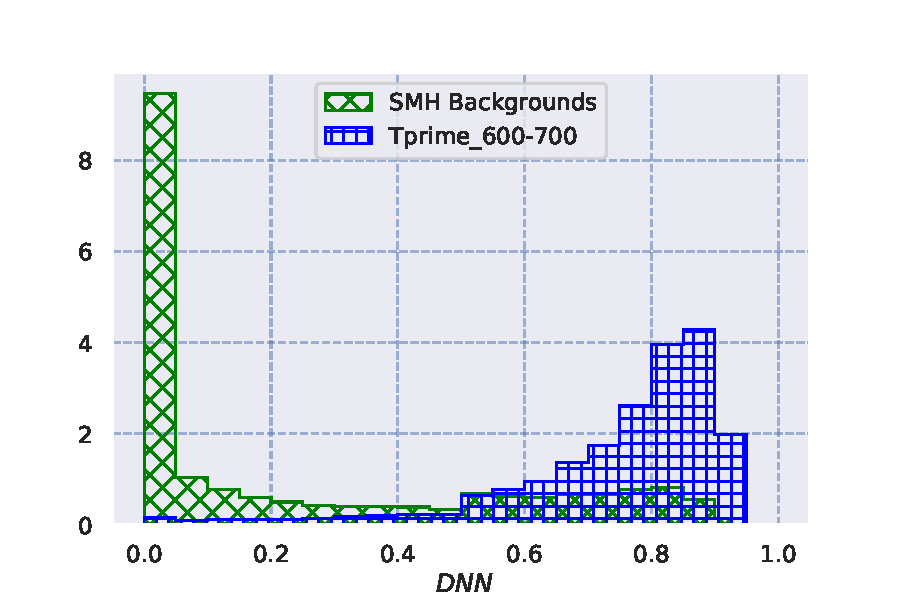
\includegraphics[width=\textwidth]{figure_4/output_TPrime600-700_on_testing_all_background.pdf}
         \caption{Tprime(600-700GeV)}
         \label{fig:y equals x}
     \end{subfigure}
     \hfill
     \begin{subfigure}[b]{0.47\textwidth}
         \centering
         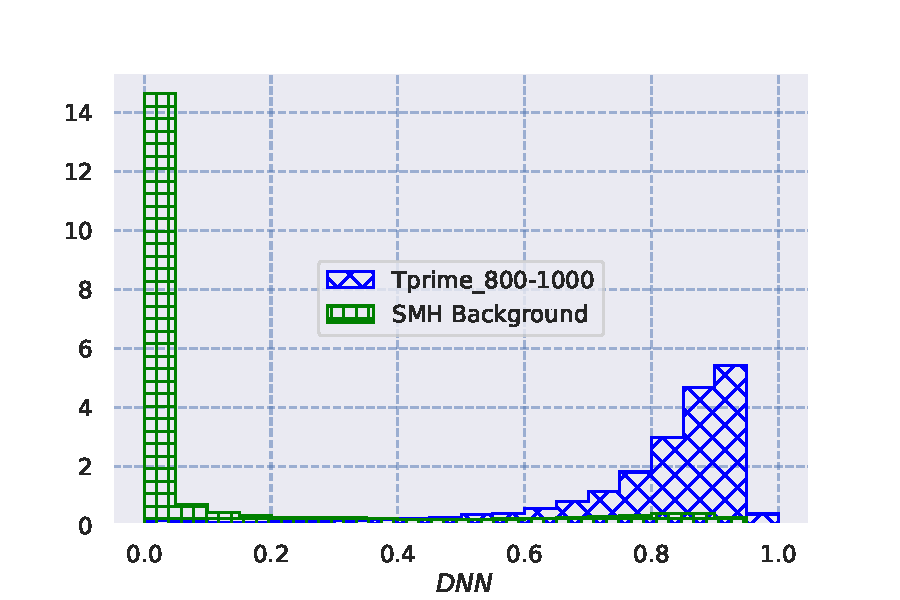
\includegraphics[width=\textwidth]{figure_4/output_TPrime800-1000_on_testing_all_background.pdf}
         \caption{Tprime(800-1000GeV)}
         \label{fig:three sin x}
     \end{subfigure}
     \hfill
     \begin{subfigure}[b]{0.47\textwidth}
         \centering
         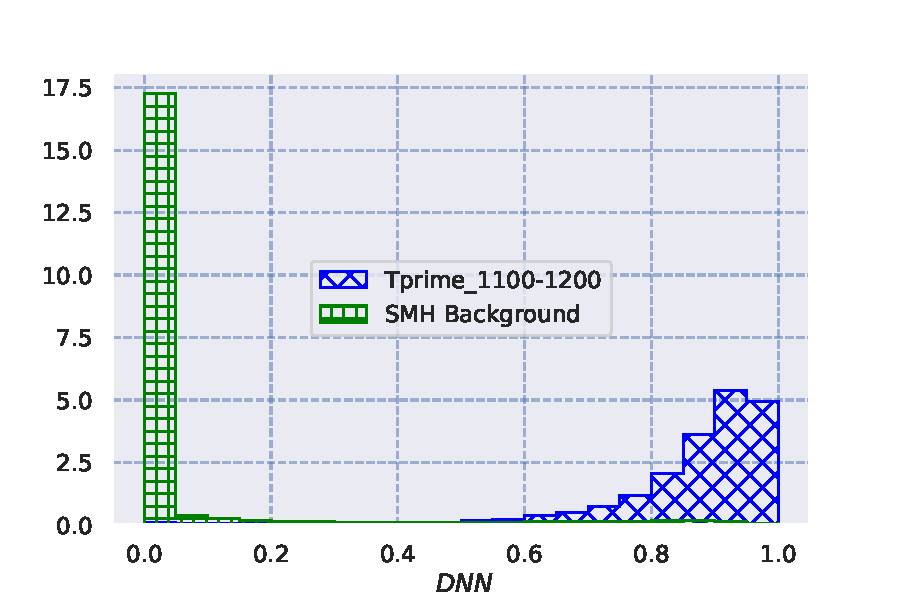
\includegraphics[width=\textwidth]{figure_4/Training_with_Tprime_1100-1200GeV_ with_backgrounds.pdf}
         \caption{Tprime(1100-1200GeV)}
         \label{fig:five over x}
     \end{subfigure}
        \caption{Separation output of signal from the background after all different training }
        \label{fig:output_training_models}
\end{figure}


To check the model training output, the corresponding output from the model has been plotted with the help of validation dataset accuracy and loss on the model. The loss of model can be interpreted as the following theoretical loss and accuracy plots as in \autoref{fig:training_and_accuracy_theo}.

\begin{figure}[H]
     \centering
     \begin{subfigure}[b]{0.4\textwidth}
         \centering
         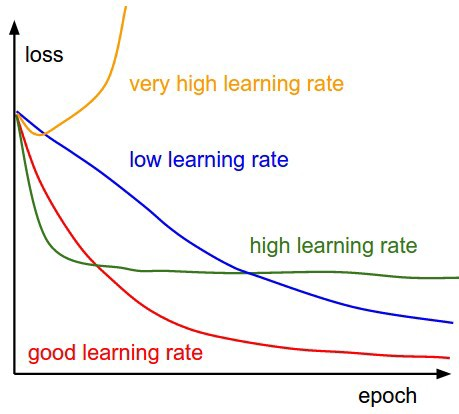
\includegraphics[width=\textwidth]{figure_4/loss.jpeg}
         \caption{loss from trained output model}
         \label{fig:y equals x}
     \end{subfigure}
     \hfill
     \begin{subfigure}[b]{0.4\textwidth}
         \centering
         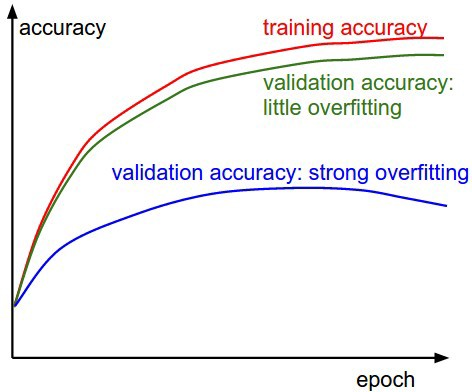
\includegraphics[width=\textwidth]{figure_4/accuracy.jpeg}
         \caption{Corresponding Accuracy}
         \label{fig:three sin x}
     \end{subfigure}

        \caption{Theoretical loss and accuracy plots\cite{ml_68}}
        \label{fig:training_and_accuracy_theo}
\end{figure}



From the \autoref{fig:output_training_models}, the model would giving a clear separation between signal and background for each model of training. Using the DNN output score, the diffent samples as discussed above were tested and output has been plotted in \autoref{fig:my_label_fig_testing}
\begin{figure}[H]
    \centering
    \includegraphics[scale=0.4]{Results_outputs/output_After_testing.png}
    \caption{Output after testing the model on the datafile, NRB, SMH, and Signals.}
    \label{fig:my_label_fig_testing}
\end{figure}



With applying weights to the input of the root file the stacked ratio plotted. To prevented the data and montecarlo mismatch, the histogram have been re-scaled with \textit{DataYield/ totalMCYield}.
 This confirms the data and monte carlo comparisons as in \autoref{fig:my_label_fig_testing}. If the data and monte carlo have mismatch then either there might be a few depressions in the data or we need to modify the theoretical predictions. 
 %%%%%%%%%%%%%%%%%%%%%%%%%%%%%%%%%%%%%%%%%%%%%%%%%%%%%%%%%$$$$$$$$$$$$$$$$$$$$$$$$$$$$$$$$$$$$$$$$$$$$$$$$$$$$$$$$$$$$$$$$$$$$$$$$$$%%%%%%%%%%%%%%%%%%%%%%%%%%%%%%%%%%%%%%%%%%%%%%%%%%%%%%%%%%%%%%%%%%%%%%%%%%%%%%%%%%%%%%%%%%%%%%%%%%%%%%%%%%%%%%%%%%%%%%%%%%%%%%%%%%%%%%%%%%%%%%%%%%%%%%%%%%%%%%%%%%%%%%%%%%%%%%










\setcounter{equation}{0}
\setcounter{table}{0}
\setcounter{figure}{0}
%\baselineskip 24pt


    
           


 




 
 

\clearpage
\chapter{\label{R_D}Results and Discussions}
The output separation of the signal and background after the training of the model are given in the \autoref{fig:output_training_models}. These training corresponds to the output with different level of separation. The level of separation are increasing from training in using Tprime[600-700 GeV] to  Tprime[1100-1200 GeV]. The training and testing accuracy can be seen in the \autoref{tab:my_label_table_1}.

% \begin{figure}[H]
%      \centering
%      \begin{subfigure}[b]{0.47\textwidth}
%          \centering
%          \includegraphics[width=\textwidth]{figure_4/output_TPrime600-700_on_testing_all_background.pdf}
%          \caption{Tprime(600-700GeV)}
%          \label{fig:y equals x}
%      \end{subfigure}
%      \hfill
%      \begin{subfigure}[b]{0.47\textwidth}
%          \centering
%          \includegraphics[width=\textwidth]{figure_4/output_TPrime800-1000_on_testing_all_background.pdf}
%          \caption{Tprime(800-1000GeV)}
%          \label{fig:three sin x}
%      \end{subfigure}
%      \hfill
%      \begin{subfigure}[b]{0.47\textwidth}
%          \centering
%          \includegraphics[width=\textwidth]{figure_4/Training_with_Tprime_1100-1200GeV_ with_backgrounds.pdf}
%          \caption{Tprime(1100-1200GeV)}
%          \label{fig:five over x}
%      \end{subfigure}
%         \caption{Separation output of signal from the background after all different training }
%   \label{fig:three graphs_11233}
% \end{figure}



% \section{Output from signal and background training}





\begin{table}[H]
    \centering
    \begin{tabular}{|c|c|c|}\hline
    Model     & Training   & Testing  \\
              & Accuracy (\%)  &     Accuracy (\%)  \\\hline
   Tprime[600-700GeV]       &     82.29        &    81.81         \\
   Tprime[800-1000GeV]          &   89.62          &     89.25        \\
   Tprime[1100-1200GeV]          &     94.76        &    94.37         \\
   Tprime[600-1200GeV]          &       87.32      &        87.14     \\\hline
    \end{tabular}
    \caption{Table with training and testing accuracy for the different training and testing with the standard model Higgs background. The output is increasing with the increase in the mass of Tprime from 600-1200GeV.}
    \label{tab:my_label_table_1}
\end{table}




The DNN model can be validated with the output receiving operator characteristic(ROC) curve for the different training from Tprime[600-700], Tprime[800-1000], and Tprime[1100-1200] can be compared with the \autoref{fig:my_label_ROC}. The ROC curve suggest the correlation between the signal and background efficiencies. This helps for the background rejections. For different training with increasing mass points of $T'$ have decreasing correlations. 
\begin{figure}[H]
    \centering
    \includegraphics{Results_outputs/ROC_curve_Comaprision_Different_training.pdf}
    \caption{ Receiving operator characteristic(ROC) curve for all the different training and testing output. The ROC area under the curve increasing with the increasing in the training of the mass point.}
    \label{fig:my_label_ROC}
\end{figure}


The output after testing of simulated samples on the DNN score from the different training are represented as in the form of stacked ratio plot as in \autoref{fig:stacked_plots_1}. All the output  after testing on standard model Higgs (SMH) backgrounds, Non-resonant backgrounds (NRBs) and on the signals corresponding to the training. The output plotted with applying the diphoton cut on  the monte carlo(MC) of the NRB and SMH, along with the datafile. The monte carlo have been scaled with the datafile as $\frac{Datafile}{MonteCarlo}$, which have been plotted as the ratio plot below the stacked histogram.\\

\begin{figure}[H]
     \centering
     \begin{subfigure}[b]{0.3\textwidth}
         \centering
         \includegraphics[width=\textwidth, scale = 0.5]{figure_4/Stacked_plot_DNN_600-700_with_diphoton_cuts.pdf}
        %  \caption{$y=x$}
        %  \label{fig:y equals x}
     \end{subfigure}
     \hfill
     \begin{subfigure}[b]{0.3\textwidth}
         \centering
         \includegraphics[width=\textwidth]{figure_4/Stacked_plot_DNN_800-1000_with_diphoton_cuts.pdf}
        %  \caption{$y=3sinx$}
        %  \label{fig:three sin x}
     \end{subfigure}
     \hfill
     \begin{subfigure}[b]{0.3\textwidth}
         \centering
         \includegraphics[width=\textwidth]{figure_4/Stacked_plot_DNN_1100-1200_with_diphoton_cuts.pdf}
        %  \caption{$y=3sinx$}
        %  \label{fig:three sin x}
     \end{subfigure}
        \caption{The stacked ratio plot corresponding to the output after testing of different backgrounds, and signal over the DNN score.}
        \label{fig:stacked_plots_1}
\end{figure}

With the help of linear fit $Y = mx+c$, the ratio plot of the data and the Monte Carlo were fitted and corresponding output of the slope and intercept, as given in \autoref{tab:my_label_DNN_1} were used to scale the values and again the stacked ratio plot were plotted as shown in the \autoref{fig:stacked_scaled_plots_DNN_200} for mismatch between the data and Monte Carlo. 


\begin{table}[H]
    \centering
    \begin{tabular}{|c|c|c|}\hline
     Model (DNN)   & Slope & Intercept \\ \hline
      TPrime[600-700]   &  -1.52828 $\pm$ 0.342382 & 2.21165 $\pm$ 0.155941  \\
       TPrime[800-1000]   &  -1.6964 $\pm$ 0.34357 & 2.2345 $\pm$ 0.139593 \\
          TPrime[1100-1200]   &  -2.34415 $\pm$ 0.477097 &  2.04436 $\pm$  0.122349  \\\hline
    \end{tabular}
    \caption{Slope and intercept after linear fitting in the DNN}
    \label{tab:my_label_DNN_1}
\end{table}




\begin{table}[H]
    \centering
    \begin{tabular}{|c|c|c|}\hline
     Model (BDT)   & Slope & Intercept \\ \hline
      TPrime[600-700]   &  -2.55526 $\pm$ 0.406623 & 2.58306 $\pm$ 0.181075  \\
       TPrime[800-1000]   &  -2.95575 $\pm$ 0.537814 & 2.50859 $\pm$ 0.182962 \\
          TPrime[1100-1200]   &  -3.16991 $\pm$ 0.483748 &  2.38726 $\pm$  0.153541  \\\hline
    \end{tabular}
    \caption{Slope and intercept after linear fitting in the BDT}
    \label{tab:my_label_BDT_table}
\end{table}



\begin{figure}[H]
     \centering
     \begin{subfigure}[b]{0.3\textwidth}
         \centering
         \includegraphics[width=\textwidth]{figure_4/Stacked_plot_DNN_600-700_with_diphoton_cuts_Scaled_inputs.pdf}
        %  \caption{$y=x$}
         \label{fig:y equals x}
     \end{subfigure}
     \hfill
     \begin{subfigure}[b]{0.3\textwidth}
         \centering
         \includegraphics[width=\textwidth]{figure_4/Stacked_plot_DNN_800-1000_with_diphoton_cuts_scaled_inputs.pdf}
        %  \caption{$y=3sinx$}
         \label{fig:three sin x}
     \end{subfigure}
    \hfill
     \begin{subfigure}[b]{0.3\textwidth}
         \centering
         \includegraphics[width=\textwidth]{figure_4/Stacked_plot_DNN_1100-1200_with_diphoton_cuts_scaled_inputs.pdf}
        %  \caption{$y=3sinx$}
         \label{fig:three sin x}
     \end{subfigure}
          \caption{The stacked ratio plot corresponding to the output after testing of different backgrounds, and signal over the DNN score after linear fitting the ratio plot and scaled the input. Here, the data are matching with the monte carlo.}
          \label{fig:stacked_scaled_plots_DNN_200}
\end{figure}



As in the DNN the process, after testing on the DNN score the coutput were plotted as the stacked 
ratio plot, the corresponding plot to the training with Boosted Decision Tree(BDT) can be seen in the
\autoref{fig:plots}. 


\begin{figure}[H]
     \centering
     \begin{subfigure}[b]{0.3\textwidth}
         \centering
         \includegraphics[width=\textwidth]{BDT_Output/Stacked_plot_BDT_600-700_with_diphoton_cuts_inputs.pdf}
        %  \caption{$y=x$}
         \label{fig:y equals x}
     \end{subfigure}
     \hfill
     \begin{subfigure}[b]{0.3\textwidth}
         \centering
         \includegraphics[width=\textwidth]{BDT_Output/Stacked_plot_BDT_800-1000_with_diphoton_cuts_inputs.pdf}
         
        %  \caption{$y=3sinx$}
         \label{fig:three sin x}
     \end{subfigure}
     \hfill
     \begin{subfigure}[b]{0.3\textwidth}
         \centering
         \includegraphics[width=\textwidth]{BDT_Output/Stacked_plot_BDT_1100-1200_with_diphoton_cuts_inputs.pdf}
        %  \caption{$y=3sinx$}
         \label{fig:three sin x}
     \end{subfigure}
        \caption{The stacked ratio plot corresponding to the output after testing of different backgrounds, and signal over the DNN score.}
        \label{fig:plots}
\end{figure}


The Stacked ration plot of BDT output after linear fit and scaling with the corresponding parameters is in \autoref{fig:BDT_ouput_Fitted_with}.

\begin{figure}
     \centering
     \begin{subfigure}[b]{0.3\textwidth}
         \centering
         \includegraphics[width=\textwidth]{BDT_Output/Stacked_plot_BDT_600-700_with_diphoton_cuts_with_scaled_inputs.pdf}
        %  \caption{$y=x$}
         \label{fig:y equals x}
     \end{subfigure}
     \hfill
     \begin{subfigure}[b]{0.3\textwidth}
         \centering
         \includegraphics[width=\textwidth]{BDT_Output/Stacked_plot_BDT_800-1000_with_diphoton_cuts_with_Scaled_inputs.pdf}
        %  \caption{$y=3sinx$}
         \label{fig:three sin x}
     \end{subfigure}
     \hfill
     \begin{subfigure}[b]{0.3\textwidth}
         \centering
         \includegraphics[width=\textwidth]{BDT_Output/Stacked_plot_BDT_1100-1200_with_diphoton_cuts_with_scaled_inputs.pdf}
        %  \caption{$y=5/x$}
         \label{fig:five over x}
     \end{subfigure}
        \caption{The stacked ratio plot corresponding to the output after testing of different backgrounds, and signal over the BDT score after linear fitting the ratio plot and scaled the input. Here, the data are matching with the monte carlo .}
        \label{fig:BDT_ouput_Fitted_with}
\end{figure}
%%%%%%%%%%%%%%%%%%%%%%%%%%%%%%%%%%%%%%%%%%%%%%%%%%%%%%%%%%%%5
%%%%%%%%%%%%%%%%%%%%%%%%%%%%%%%%%%%%%%%%%%%%%%%%%%%%%%%%%%%%5
%%%%%%%%%%%%%%%%%%%%%%%%%%%%%%%%%%%%%%%%%%%%%%%%%%%%%%%%%%%%5
%%%%%%%%%%%%%%%%%%%%%%%%%%%%%%%%%%%%%%%%%%%%%%%%%%%%%%%%%%%%5
%%%%%%%%%%%%%%%%%%%%%%%%%%%%%%%%%%%%%%%%%%%%%%%%%%%%%%%%%%%%5
%%%%%%%%%%%%%%%%%%%%%%%%%%%%%%%%%%%%%%%%%%%%%%%%%%%%%%%%%%%%5
%%%%%%%%%%%%%%%%%%%%%%%%%%%%%%%%%%%%%%%%%%%%%%%%%%%%%%%%%%%%5


\section{BDT and DNN Comparisons}\label{sec:comp}
The different machine learning techniques comparisons can be seen in the following figures.

\begin{figure}[H]
     \centering
     \begin{subfigure}[b]{0.45\textwidth}
         \centering
         \includegraphics[width=\textwidth]{figure_4/Stacked_plot_DNN_600-700_with_diphoton_cuts.pdf}
        %  \caption{$y=x$}
         \label{fig:y equals x}
     \end{subfigure}
     \hfill
     \begin{subfigure}[b]{0.45\textwidth}
         \centering
         \includegraphics[width=\textwidth ]{BDT_Output/Stacked_plot_BDT_600-700_with_diphoton_cuts_inputs.pdf}
        %  \caption{$y=3sinx$}
         \label{fig:three sin x}
     \end{subfigure}
     \label{fig:Comaprision_1}
     \caption{Comparison for the BDT and DNN output corresponding to the training for Tprime[600-700GeV] and testing on NRB, SMH, and Tprime at 600GeV and 700GeV as given in \autoref{tab:my_label_DNN_1} and \autoref{tab:my_label_BDT_table}.}
\end{figure}




\begin{figure}[H]
     \centering
     \begin{subfigure}[b]{0.47\textwidth}
         \centering
         \includegraphics[width=\textwidth]{figure_4/Stacked_plot_DNN_800-1000_with_diphoton_cuts.pdf}
        %  \caption{$y=x$}
         \label{fig:y equals x}
     \end{subfigure}
     \hfill
     \begin{subfigure}[b]{0.47\textwidth}
         \centering
         \includegraphics[width=\textwidth]{BDT_Output/Stacked_plot_BDT_800-1000_with_diphoton_cuts_inputs.pdf}
        %  \caption{$y=3sinx$}
         \label{fig:three sin x}
     \end{subfigure}
     \label{fig:Comaprision_2}
     \caption{Comparison for the BDT and DNN output corresponding to the training for Tprime[800-1000GeV] and testing on NRB, SMH, and Tprime at 600GeV, 700GeV, 900GeV, and 1000GeV as given in \autoref{tab:my_label_DNN_1} and \autoref{tab:my_label_BDT_table}.}
\end{figure}




\begin{figure}[H]
     \centering
     \begin{subfigure}[b]{0.47\textwidth}
         \centering
         \includegraphics[width=\textwidth]{figure_4/Stacked_plot_DNN_1100-1200_with_diphoton_cuts.pdf}
        %  \caption{$y=x$}
         \label{fig:y equals x}
     \end{subfigure}
     \hfill
     \begin{subfigure}[b]{0.47\textwidth}
         \centering
         \includegraphics[width=\textwidth]{BDT_Output/Stacked_plot_BDT_1100-1200_with_diphoton_cuts_inputs.pdf}
        %  \caption{$y=3sinx$}
         \label{fig:three sin x}
     \end{subfigure}
    \hfill
     \label{fig:Comaprision_3}
     \caption{Comparison for the BDT and DNN output corresponding to the training for Tprime[1100-1200GeV] and testing on NRB, SMH, and Tprime at 600GeV, 700GeV, 1100GeV, and 1200GeV as given in \autoref{tab:my_label_DNN_1} and \autoref{tab:my_label_BDT_table}.}
\end{figure}

%%%%%%%%%%%%%%%%Scaled Inputs%%%%%%%%%%%%%%%%%%%%


\begin{figure}[H]
     \centering
     \begin{subfigure}[b]{0.47\textwidth}
         \centering
         \includegraphics[width=\textwidth]{figure_4/Stacked_plot_DNN_600-700_with_diphoton_cuts_Scaled_inputs.pdf}
        %  \caption{$y=x$}
         \label{fig:y equals x}
     \end{subfigure}
     \hfill
     \begin{subfigure}[b]{0.47\textwidth}
         \centering
         \includegraphics[width=\textwidth]{BDT_Output/Stacked_plot_BDT_600-700_with_diphoton_cuts_inputs.pdf}
        %  \caption{$y=3sinx$}
         \label{fig:three sin x}
     \end{subfigure}
    \hfill
     \label{fig:Comaprision_4}
     \caption{Comparision for the BDT and DNN output corresponding to the training for Tprime[600-700GeV] and testing on NRB, SMH, and Tprime at 600GeV and 700GeV with the scaled inputs after fitted parameter of slope and intercept as given in \autoref{tab:my_label_DNN_1} and \autoref{tab:my_label_BDT_table}.}
\end{figure}






\begin{figure}[H]
     \centering
     \begin{subfigure}[b]{0.47\textwidth}
         \centering
         \includegraphics[width=\textwidth]{figure_4/Stacked_plot_DNN_800-1000_with_diphoton_cuts_scaled_inputs.pdf}
        %  \caption{$y=x$}
         \label{fig:y equals x}
     \end{subfigure}
     \hfill
     \begin{subfigure}[b]{0.47\textwidth}
         \centering
         \includegraphics[width=\textwidth]{BDT_Output/Stacked_plot_BDT_800-1000_with_diphoton_cuts_with_Scaled_inputs.pdf}
        %  \caption{$y=3sinx$}
         \label{fig:three sin x}
     \end{subfigure}
    \hfill
     \label{fig:}
     \caption{Comparison for the BDT and DNN output corresponding to the training for Tprime[800-1000GeV] and testing on NRB, SMH, and Tprime at 600GeV, 700GeV, 900GeV, and 1000GeV with the scaled inputs after fitted parameter of slope and intercept as given in \autoref{tab:my_label_DNN_1} and \autoref{tab:my_label_BDT_table}.}
\end{figure}



\begin{figure}[H]
     \centering
     \begin{subfigure}[b]{0.47\textwidth}
         \centering
         \includegraphics[width=\textwidth]{figure_4/Stacked_plot_DNN_1100-1200_with_diphoton_cuts_scaled_inputs.pdf}
        %  \caption{$y=x$}
         \label{fig:y equals x}
     \end{subfigure}
     \hfill
     \begin{subfigure}[b]{0.47\textwidth}
         \centering
         \includegraphics[width=\textwidth]{BDT_Output/Stacked_plot_BDT_1100-1200_with_diphoton_cuts_with_scaled_inputs.pdf}
        %  \caption{$y=3sinx$}
         \label{fig:three sin x}
     \end{subfigure}
    \hfill
     \label{fig:}
     \caption{Comparison for the BDT and DNN output corresponding to the training for Tprime[1100-1200GeV] and testing on NRB, SMH, and Tprime at 600GeV, 700GeV, 1100GeV, and 1200GeV with the scaled inputs after fitted parameter of slope and intercepts as given in \autoref{tab:my_label_DNN_1} and \autoref{tab:my_label_BDT_table}.}
\end{figure}








 \section{Limit Calculation}\label{sec:limit_Ca}
Before the use of higgs combine tools on the output variable of the DNN and applying cuts these are the number of the events. This is a frequentist hypothesis to calculate the probability of an hypothesis to be inferred from the data based on a large set of hypothetical experiments, such as the Monte Carlo. 
for the blinded region analysis on 115 < $m_{\gamma\gamma}$ < 135GeV on the monte carlo samples of backgrounds(NRB) have been scaled after the linear fitting of the $\frac{Data}{MC}$ ratio, and scaled to match the data and monte carlo. 
With the cuts applied as in \autoref{tab:my_label_cuts}, the background have been rejected to get most of the signal processes afer testing over the DNN score. 


\begin{table}[H]
    \centering
    \begin{tabular}{c|c} \hline
     Model &  Cuts Applied(position)\\\hline
      ${T'}$[600,700]   &  0.54\\
      $T'$[800,1000]   & 0.76 \\
      $T'$[1100,1200] & 0.80 \\\hline
    \end{tabular}
    \caption{Different cuts applied for different training}
    \label{tab:my_label_cuts}
\end{table}

The inputs sample have been scaled after linear fitting of the ratio plot or applied cuts with following strategy for all the different training of $T{^'}$[600, 700]$\cup$,$T{^'}$[800, 1000]$\cup$, and  $T{^'}$[1100, 1200]. 
\begin{table}[H]
    \centering
    \begin{tabular}{c|c}\hline
     Samples    &  \\\hline
     Signals    & Only DNN Cut \\
     NRB        & DNN cut and scaled input after linear fit \\
     SMH        & Only DNN cut \\\hline
    \end{tabular}
    \caption{Different analysis strategy for applying cuts for different model before passing to the Higgs combine tools for limit calculations.}
    \label{tab:my_label}
\end{table}





% The problem of probability density estimation in principle can be solved quite simply! One would merely histogram the multivariate data x in M bins in each of the d feature variables. The fraction of events 
% (points) that fall within each bin yields a direct estimate of the density at the value of the feature
% vector x, say at the center of the bin. The bin width (and therefore the number of bins M) has to be chosen such that the structure in the density is not washed out (due to too few bins) and the density estimation is not too spiky (due to too many bins). The serious disadvantage of the histogramming method is that the total number of bins required grows like $M_d$ (referred to as Bellman’s curse of dimensionality). We would
% require a huge number of data points or else most of
% the bins would be empty leading to an estimated
% density of zero for those bins. The other issue is that
% the variables are generally correlated, and tend to be
% restricted to a sub-space of lower dimensionality,
% referred to as intrinsic dimensionality. Clearly, this
% method is inadequate for high dimensional data. There
% are better and more efficient methods for density
% estimation.

The discriminant observable, $S_T$, is used to test the presence of signal by performing
a binned likelihood fitting. The statistical analysis is based on a binned likelihood function L($\mu$, $\theta$) as constructed in  as a product of Poisson probability functions($Poiss(n_i; \mu_{s_i} + b_i)$) over all bins of the used distributions. The signal strength $\mu$ is a multiplicative factor for the signal production cross-section and is regarded as the Parameter of
Interest (POI). For each bin, $n_i$ denotes the observed data while $s_i$ and $b_i$ represent the predicted signal and background contribution from MC in the corresponding bin that depend
on a set of nuisance parameters (NPs), $\theta$, encoding the effect of systematic uncertainties
\begin{equation}
    \mathcal{L(\mu, \theta)} = \pi_{i=1}^N_{bins}Pois(n_i;\mu s_i +b_i)\times P(\theta) 
\end{equation}

In a counting experiment, let's take example for the Higgs, the Higgs hypothesis is that of signal $s(m_H)$\\
\begin{equation*}
    s(m_H) = L\sigma_{SM}.A.\epsilon
\end{equation*}
Where, L is the integrated luminosity, sigma is the standard model cross section  with A is the acceptance, and $\epsilon$ is the efficiency. 
In the counting experiment, the number of events is,
\begin{equation*}
    n = \mu s(m_H) + b
\end{equation*}

\begin{equation}\label{eq:my_eqn_12}
    \mu = \frac{L \sigma_{obs}(m_H)}{L \sigma_{SM}(m_H)} = \frac{\sigma_{obs}(m_H)}{\sigma_{SM}(m_H)}
\end{equation}

Where, $\mu$ is the strength of the signal(with respect to the expected standard model one).




The Higgs combined tools used for the calculation of expected limit on each of the $T'$ mass points, the CMS environment used for the analysis were under the \textit{CMSSW 12\_4}\cite{ml_70}. The parameter $\mu$ is varying at each of the mass points, which is plotted in \autoref{fig:my_label_limit}.Combine is used over the prepared data-card for the calculation of the expected limits.




The mean(50\%) corresponding to expected limit for two different machine learning techniques Deep Neural Network(DNN) and Boosted Decision Trees(BDT) are shown in \autoref{tab:my_label_Comparision_BDT_DNN}

\begin{table}[H]
    \centering
    \begin{tabular}{c|c|c}\hline
     Events    & Mean(DNN)  & Mean(BDT)  \\\hline
     Tprime 600    &  6.9062  & 7.9688 \\
     Tprime 625 & 7.2188     &  8.6875  \\
     Tprime 650 & 8.0625  &   9.6875   \\
     Tprime 675 & 9.1562  & 10.8438 \\
     Tprime 700 & 10.4375 & 11.9375 \\
     Tprime 800 & 10.3125 & 7.375  \\
     Tprime 900 & 17.5 & 10.1875   \\
     Tprime 1000 & 19.6875 & 15.0625 \\
     Tprime 1100 & 17.1875 & 21.6875 \\
     Tprime 1200 & 23.9375 & 29.75 \\\hline
    \end{tabular}
    \caption{Table with all the mean value of the DNN and BDT at the corresponding mass of the Tprime from 600 to 1200GeV.}
    \label{tab:my_label_Comparision_BDT_DNN}
\end{table}








The table \autoref{tab:my_label_table_11} containing all the input variables at each mass point for the combined limit calculations for the training Tprime[800-1000]. 
\begin{table}[h]
    \centering
    \resizebox{\textwidth}{!}{
    \begin{tabular}{|cccc|}\hline
     Process    & Number of events & Number of events & Number of events  \\ 
                & before applying diphoton cuts & after applying diphoton cuts & before limit calculation \\ \hline \hline
                 DataFile        &     2400      &    1647     &      1647    \\
                  &           &         &          \\
     Tprime 600        &     81013      &   81013      &    -      \\
      Tprime 700        &     92703      &  92703       &     -     \\
       Tprime 800        &     101761      &    101761     &   61834       \\
        Tprime 900        &   100962        &   100962      &     81552     \\
         Tprime 1000        &     105546      &   105546      &   92489       \\
          Tprime 1100        &     91543      &    91543     &       -   \\
           Tprime 1200        &    107628       &    107628     &      -    \\
               &           &         &          \\\hline \hline
     ttgg          &    55847       &    39314     &   18016       \\
     ttjets         &   1320        &   904      &     642     \\
     diphotongamma         &    8323       &  5811       &    2882      \\
     gjets          &      228     &  151       &     86     \\
     ttgjets          &   9441        &    6574     &     3375     \\
               &           &         &          \\\hline \hline
        thq       &   338874        &         &    89800      \\
       tth        &   92486        &         &     19000     \\
       vbf        &     1199      &         &    235      \\
        vh              &   8080        &         &    1174      \\        
        ggh       &    529       &         &      111    \\ \hline
    \end{tabular}}
    \caption{The number of events corresponding output at dufferent position in the course of training that is number of events before applying diphoton cut, number of events after applying diphoton cuts and before the limit exclusion plot through datacard preparation for DNN Tprime 800-1000}
    \label{tab:my_label_table_11}
\end{table}











%%%%%%%%%%%%%%%%%%%%%%%%%%%%%%%%%%%%%%%%%%%%%%%%%%%%%%%%%%%%%%%%%%%%%%%%%%%%%%%%%%%%%%%%%%%%%%%%%%%%%%%%%%%%%%%%%%%%%%%%%%%%%%%%%%%%%%%%%%%%%%%%%%%%%%%%%%%%%%%%%%%%%%%%%%%%%%%%%%%%%%%%%%%%%%%%%%%%%%%%%%%%%%%%%%%%%%%%%%%%%%%%%%%%%%%%%%%%%%%%%%%%%%%%%%%%%%%%%%%%%%%%%%%%%%%%%%%%%%%%%%%%%%%%%%%%%%%%%%%%%%%%%%%%%%%%%%%%%%%%%%%%%%%%%%%%%%%%%%%%%%%%%%%%%%%%%%%%%%%%%%%%%%%%%%%%%%


The expected limit are derived using a simultaneous maximum likelihood fit of the $m_{\gamma\gamma}$ distributions in the signal regions defined for the leptonic channels for each of $T'$ mass point ranging from 600 to 1200 GeV. Limits are calculated at 95\% CL with the asymptotic statistical method using the combine tool. The expected limits on signal strength for each $T’$ mass hypothesis of the DNN in comparison with the BDT, can be seen  from the \autoref{fig:my_label_limit}. 

\begin{figure}[H]
    \centering
    \includegraphics[scale=0.8]{figure_4/muALL_Plot_600-1200_ .pdf}
    \caption{Expected 95\% CL limits for signal strength($\mu$) in the leptonic channel with comparison to the output of the BDT with $M_{T'}$ $\in$ [600, 1200]GeV.}
    \label{fig:my_label_limit}
\end{figure}

The expected limit on the ${T'}$ production cross-section are evaluated through \autoref{eq:1.1}, which is similar to the \autoref{eq:my_eqn_12}. The combined result together with the BDT comparison can be seen in the \autoref{fig:my_label_Comparision}.
\begin{equation} \label{eq:1.1}
    \sigma_{upper\ limit} = \mu_{upper\ limit} \times \sigma_{theory}
\end{equation}


\begin{figure}[H]
    \centering
    \includegraphics[scale=0.8]{figure_4/muALL_Plot_600-1200_with_cross_Section_comparision.pdf}
    \caption{Expected 95\% CL limits for $\sigma \times$ BR(H$\longrightarrow$$\gamma\gamma$)  in the leptonic channel with comparison to the output of the BDT with $M_{T'}$ $\in$ [600, 1200]GeV.}
    \label{fig:my_label_Comparision}
\end{figure}






% \url{https://cds.cern.ch/record/2789988?ln=en}
% \url{https://cdsweb.cern.ch/search?ln=en&cc=Theses&sc=1&p=VLQ&action_search=Search&op1=a&m1=a&p1=&f1=}
























% \section{Correlation between signal and background variable}
% A correlation function represents a measurement between the strength of a linear relationship between two quantitative variables. There are two types of correlation, positive correlation and negative correlation. Positive correlation represents a relationship between two variables in which both variables move in the same direction. This means when one variable increases while the other also increases and vice versa While negative correlation is a relationship where one variable increases as the other decreases, and vice versa. A correlation of 1 or +1 shows a perfect positive correlation, which means both the variables move in the same direction. A correlation of -1 shows a perfect negative correlation, which means as one variable goes down, the other goes up \cite{27}. Here for the comparison of the variables (given in \autoref{tab:my_label_1}) from two different datasets were calculated using Pearson Correlation Coefficient Formula, which is,
% \begin{equation}
%     r = \frac{n(\sum xy)- \sum x \sum y}{\sqrt{[n \sum x^2 - (\sum x)^2][n \sum y^2 - (\sum y)^2]}}
% \end{equation}
% Where,\\
% n = Quantity of Information \\
% $\sum x$ = Total of the First Variable Value \\
% $\sum y$ = Total of the Second Variable Value\\
% $\sum xy$ = Sum of the Product of first \& Second Value\\
% $\sum x^2$ = Sum of the Squares of the First Value\\
% $\sum y^2$ = Sum of the Squares of the Second Value\\

















\setcounter{equation}{0}
\setcounter{table}{0}
\setcounter{figure}{0}
%\baselineskip 24pt


    




\clearpage
\chapter{\label{summary}Summary and Conclusion}
In this project, machine learning techniques(Deep Neural Network) have been explored to classify data from CMS, CERN as the signal events from the backgrounds. We mainly focused on simulated Monte Carlo data samples produced after PP collision at the center of mass energy ($\sqrt{s}$) 13TeV at the integrated luminosity of 137 $fb^{-1}$. A few of the samples produced are Tprime $T'$, Standard model Higgs(SMH), and the Non-Resonant backgrounds(NRB) are used for the analysis. The DNN model training has been done for three different ranges of mass points of $T'$([600,700]$\cup$[800, 1000]$\cup$ [1100, 1200]) as the signals while the SMH as the the backgrounds for the better sensitivity of the DNN model. The advantages of using deep neural networks (DNN) for training  as it updates all the parameters itself to give a better optimized outputs by updating its weights using back propagation methods after each iteration or the epochs.

In this analysis, extensively studied multivariate techniques to separate arbitrary signal (T$'$) from the standard model Higgs(SMH) backgrounds processes using the CMS detector simulation and the reconstruction program. In the machine learning training, model separation of signals and backgrounds seems to be getting better with increasing mass of the $T'$.  The DNN training output score used to tests over the different simulated datasets and plotted as the stacked ratio plot. To scale the data and the Monte Carlo, the Monte Carlo samples have been scaled with corresponding outputs from the linear fit of the ratio plot.  

In this blinded analysis with 115 < $m_{\gamma\gamma}< 135$GeV, with the cuts applied to separate signal events from the backgrounds and further scaling the NRB backgrounds with scaling parameters, all the Monte Carlo were rescaled. The performance of DNN has been well evaluated over the Non Resonant background processes. Using Higgs Combined Tools under CMMSW environment, the expected limit at 95\% CL on $T'$ production processes have been extracted at each $T'$ mass in the range
[600,1200] using the DNN based selection criteria, as well as for the present CMS analysis(BDT). 

The output comparison from both the DNN and BDT output cannot able to give a concrete output. The NN-based analysis sensitivity is yet to reach the exclusion potential.
% searched for single produced vector-like T quarks decaying at $\sqrt{s}$ = 13 TeV. Here, an analysis to look for $T{^'} \longrightarrow$ top + H with H$\longrightarrow \gamma \gamma$. This analysis is composed on leptonic channel only and is based on DNNs to seperate the signal $T^'$ from the major backgrounds. Expected limits have been calculated for the DNN output variables. The predicted limit output from the DNN, compared with the expected limits of the another machine learning techniques, BDT, 

By the end of 2025, LHC is supposed to be upgraded to high luminosity LHC(HL-LHC) which is supposed to have collected data with an integrated luminosity of 3000 $fb^{-1}$. With the higher luminosity, a new analysis can be performed using sophisticated machine learning techniques to have more signal significance. With more data, we hope to discover some exciting new physics!
\setcounter{equation}{0}
\setcounter{table}{0}
\setcounter{figure}{0}
%\baselineskip 24pt


    





%\clearpage
%\addcontentsline{toc}{chapter}{Appendices}
\begin{appendices}
\chapter{\label{appendix}}
\end{appendices}

\section{Comparison with the increasing number of layers}
How to select number of layers for the DNN model? With the fixed number of 512 nodes in each layer, the corresponding output comparison can be seen in \autoref{tab:app_1}

\begin{table}[H]
    \centering
    \begin{tabular}{c|c|c} \hline
      \# of Layers in the DNN  & Training Accuracy(\%) &  Testing Accuracy (\%)  \\ \hline \hline
      
       One(NN)        &     80.24   &    79.97  \\
       Two      &  82.15 & 81.59    \\
        Three    & 82.68 & 82.08  \\
        Four &  82.49 & 81.94 \\\hline \hline
    \end{tabular}
    \caption{Training and testing accuracy after training with simulated samples of Tprime(600-700GeV) with the standard model Higgs(SMH) backgrounds with each layer having 512 nodes.}
    \label{tab:app_1}
\end{table}






\subsection{One layer Only}
\begin{figure}[H]
     \centering
     \begin{subfigure}[b]{0.3\textwidth}
         \centering
         \includegraphics[width=\textwidth]{figure_3/One_node_only_accuracy.pdf}
         \caption{Model Accuracy}
         \label{fig:y equals x}
     \end{subfigure}
     \hfill
     \begin{subfigure}[b]{0.3\textwidth}
         \centering
         \includegraphics[width=\textwidth]{figure_3/One_node_only_loss.pdf}
         \caption{Model Loss}
         \label{fig:three sin x}
     \end{subfigure}
     \hfill
     \begin{subfigure}[b]{0.3\textwidth}
         \centering
         \includegraphics[width=\textwidth]{figure_3/one_layer_only_ROC.pdf}
         \caption{Model ROC Curve}
         \label{fig:five over x}
     \end{subfigure}
        \caption{Output corresponding to the training with only one layer(NN)}
        \label{fig:three graphs}
\end{figure}


\subsection{Two layers }
\begin{figure}[H]
     \centering
     \begin{subfigure}[b]{0.3\textwidth}
         \centering
         \includegraphics[width=\textwidth]{figure_3/One_node_two_accuracy.pdf}
         \caption{Model Accuracy}
         \label{fig:y equals x}
     \end{subfigure}
     \hfill
     \begin{subfigure}[b]{0.3\textwidth}
         \centering
         \includegraphics[width=\textwidth]{figure_3/One_node_two_loss.pdf}
         \caption{Model loss}
         \label{fig:three sin x}
     \end{subfigure}
     \hfill
     \begin{subfigure}[b]{0.3\textwidth}
         \centering
         \includegraphics[width=\textwidth]{figure_3/two_layer_only_ROC.pdf}
         \caption{Model ROC Curve }
         \label{fig:five over x}
     \end{subfigure}
        \caption{Output corresponding to the training with two layers}
        \label{fig:three graphs}
\end{figure}


\subsection{Three layers}
\begin{figure}[H]
     \centering
     \begin{subfigure}[b]{0.3\textwidth}
         \centering
         \includegraphics[width=\textwidth]{figure_3/One_node_three_accuracy.pdf}
         \caption{Model Accuracy}
         \label{fig:y equals x}
     \end{subfigure}
     \hfill
     \begin{subfigure}[b]{0.3\textwidth}
         \centering
         \includegraphics[width=\textwidth]{figure_3/One_node_three_loss.pdf}
         \caption{Model loss}
         \label{fig:three sin x}
     \end{subfigure}
     \hfill
     \begin{subfigure}[b]{0.3\textwidth}
         \centering
         \includegraphics[width=\textwidth]{figure_3/three_layer_only_ROC.pdf}
         \caption{Model ROC Curve}
         \label{fig:five over x}
     \end{subfigure}
        \caption{Output corresponding to the training with three layers}
        \label{fig:three graphs}
\end{figure}




\subsection{Four layers}
\begin{figure}[H]
     \centering
     \begin{subfigure}[b]{0.3\textwidth}
         \centering
         \includegraphics[width=\textwidth]{figure_3/One_node_four_accuracy.pdf}
         \caption{Model Accuracy}
         \label{fig:y equals x}
     \end{subfigure}
     \hfill
     \begin{subfigure}[b]{0.3\textwidth}
         \centering
         \includegraphics[width=\textwidth]{figure_3/One_node_four_loss.pdf}
         \caption{Model Loss}
         \label{fig:three sin x}
     \end{subfigure}
     \hfill
     \begin{subfigure}[b]{0.3\textwidth}
         \centering
         \includegraphics[width=\textwidth]{figure_3/four_layer_only_ROC.pdf}
         \caption{Model ROC Curve}
         \label{fig:five over x}
     \end{subfigure}
        \caption{Output corresponding to the training with four layers}
        \label{fig:three graphs}
\end{figure}





\subsubsection{Comparison of ROC}
\begin{figure}[h]
    \centering
    \includegraphics{figure_3/comaprision_ROC_with_layer_only_ROC.pdf}
    \caption{ROC comparison for different number of layers after keeping all other parameters for the DNN training constant. The ROC curve increases from single layer to two layer, while it get remains constant up to the four layers. On further increasing the number of layers, the model get overfit and the ROC-AUC decreases, which is also evident from \autoref{tab:app_1}}
    \label{fig:my_label}
\end{figure}



\setcounter{equation}{0}
\setcounter{table}{0}
\setcounter{figure}{0}
%\baselineskip 24pt


    



                              


\bibliography{ref}
\bibliographystyle{ieeetr}

% %}
\end{document}
